\documentclass[12pt]{amsart}

% PACKAGES
\usepackage{amsmath}
\usepackage{amssymb}
\usepackage{amsfonts}
\usepackage[alphabetic]{amsrefs}
\usepackage{amsthm}
\usepackage{enumitem}
\setlist[enumerate,1]{left=0pt,label=(\arabic*)}
%\usepackage{enumerate}
\usepackage{fullpage}
\usepackage{color}
\usepackage{graphicx}
\usepackage{wrapfig}
\usepackage{hyperref}
\usepackage{microtype}
\usepackage{correctmathalign}
\usepackage{tikz}
\usepackage{pgfplots}
\pgfplotsset{compat=1.17}
\usepackage{float}
\usepackage{caption}
\usepackage{quiver}
%\usepackage{lipsum}
%\hypersetup{linktoc = all, colorlinks = true, urlcolor = Blue, linkcolor = Red, citecolor = RoyalBlue}
%\usepackage[parfill]{parskip}


% COMMANDS 
\newcommand{\nc}{\newcommand}
\newcommand{\rc}{\renewcommand}
\nc{\on}{\operatorname}

% EDITING
\definecolor{red}{rgb}{1,0,0}
\definecolor{orange}{rgb}{1,0.5,0}
\definecolor{purple}{rgb}{.5,.2,.8}
\definecolor{blue}{rgb}{.2,.2,.8}
\definecolor{green}{rgb}{.4,.6,.4}
\definecolor{myorange}{RGB}{235, 129, 27}
\newcommand{\question}[1]{\noindent  \textcolor{red}{Question: #1}}
\newcommand{\todo}[1]{\noindent  \textcolor{blue}{To do: #1}}

% Editing line spacing
%\linespread{1.5}

% BLACKBOARD BOLD
\rc{\AA}{\mathbb{A}}	
\nc{\BB}{\mathbb{B}}	
\nc{\CC}{\mathbb{C}}	
\nc{\DD}{\mathbb{D}}	
\nc{\EE}{\mathbb{E}}	
\nc{\FF}{\mathbb{F}}	
\nc{\GG}{\mathbb{G}}	
\nc{\HH}{\mathbb{H}}	
\nc{\II}{\mathbb{I}}	
\nc{\JJ}{\mathbb{J}}	
\nc{\KK}{\mathbb{K}}	
\nc{\LL}{\mathbb{L}}	
\nc{\MM}{\mathbb{M}}	
\nc{\NN}{\mathbb{N}}	
\nc{\OO}{\mathbb{O}}	
\nc{\PP}{\mathbb{P}}	
\nc{\QQ}{\mathbb{Q}}	
\nc{\RR}{\mathbb{R}}	
\rc{\SS}{\mathbb{S}}	
\nc{\TT}{\mathbb{T}}	
\nc{\UU}{\mathbb{U}}	
\nc{\VV}{\mathbb{V}}	
\nc{\WW}{\mathbb{W}}	
\nc{\XX}{\mathbb{X}}	
\nc{\YY}{\mathbb{Y}}	
\nc{\ZZ}{\mathbb{Z}}	

% BOLD FACE
\nc{\bA}{\mathbf{A}}	
\nc{\bB}{\mathbf{B}}	
\nc{\bC}{\mathbf{C}}	
\nc{\bD}{\mathbf{D}}	
\nc{\bE}{\mathbf{E}}	
\nc{\bF}{\mathbf{F}}	
\nc{\bG}{\mathbf{G}}	
\nc{\bH}{\mathbf{H}}	
\nc{\bI}{\mathbf{I}}	
\nc{\bJ}{\mathbf{J}}	
\nc{\bK}{\mathbf{K}}	
\nc{\bL}{\mathbf{L}}	
\nc{\bM}{\mathbf{M}}	
\nc{\bN}{\mathbf{N}}	
\nc{\bO}{\mathbf{O}}	
\nc{\bP}{\mathbf{P}}	
\nc{\bQ}{\mathbf{Q}}	
\nc{\bR}{\mathbf{R}}	
\nc{\bS}{\mathbf{S}}	
\nc{\bT}{\mathbf{T}}	
\nc{\bU}{\mathbf{U}}	
\nc{\bV}{\mathbf{V}}	
\nc{\bW}{\mathbf{W}}	
\nc{\bX}{\mathbf{X}}	
\nc{\bY}{\mathbf{Y}}	
\nc{\bZ}{\mathbf{Z}}	

% CALLIGRAPHIC
\nc{\calA}{\mathcal{A}}	
\nc{\calB}{\mathcal{B}}	
\nc{\calC}{\mathcal{C}}	
\nc{\calD}{\mathcal{D}}	
\nc{\calE}{\mathcal{E}}	
\nc{\calF}{\mathcal{F}}	
\nc{\calG}{\mathcal{G}}	
\nc{\calH}{\mathcal{H}}	
\nc{\calI}{\mathcal{I}}	
\nc{\calJ}{\mathcal{J}}	
\nc{\calK}{\mathcal{K}}	
\nc{\calL}{\mathcal{L}}	
\nc{\calM}{\mathcal{M}}	
\nc{\calN}{\mathcal{N}}	
\nc{\calO}{\mathcal{O}}	
\nc{\calP}{\mathcal{P}}	
\nc{\calQ}{\mathcal{Q}}	
\nc{\calR}{\mathcal{R}}	
\nc{\calS}{\mathcal{S}}
\nc{\calT}{\mathcal{T}}	
\nc{\calU}{\mathcal{U}}	
\nc{\calV}{\mathcal{V}}	
\nc{\calW}{\mathcal{W}}
\nc{\calX}{\mathcal{X}}	
\nc{\calY}{\mathcal{Y}}	
\nc{\calZ}{\mathcal{Z}}

% LOWERCASE FRAK
\nc{\fraka}{\mathfrak{a}}
\nc{\frakb}{\mathfrak{b}}
\nc{\frakc}{\mathfrak{c}}
\nc{\frakd}{\mathfrak{d}}
\nc{\frake}{\mathfrak{e}}
\nc{\frakf}{\mathfrak{f}}
\nc{\frakg}{\mathfrak{g}}
\nc{\frakh}{\mathfrak{h}}
\nc{\fraki}{\mathfrak{i}}
\nc{\frakj}{\mathfrak{j}}
\nc{\frakk}{\mathfrak{k}}
\nc{\frakl}{\mathfrak{l}}
\nc{\frakm}{\mathfrak{m}}
\nc{\frakn}{\mathfrak{n}}
\nc{\frako}{\mathfrak{o}}
\nc{\frakp}{\mathfrak{p}}
\nc{\frakq}{\mathfrak{q}}
\nc{\frakr}{\mathfrak{r}}
\nc{\fraks}{\mathfrak{s}}
\nc{\frakt}{\mathfrak{t}}
\nc{\fraku}{\mathfrak{u}}
\nc{\frakv}{\mathfrak{v}}
\nc{\frakw}{\mathfrak{w}}
\nc{\frakx}{\mathfrak{x}}
\nc{\fraky}{\mathfrak{y}}
\nc{\frakz}{\mathfrak{z}}

% UPPERCASE FRAK
\nc{\frakA}{\mathfrak{A}}
\nc{\frakB}{\mathfrak{B}}
\nc{\frakC}{\mathfrak{C}}
\nc{\frakD}{\mathfrak{D}}
\nc{\frakE}{\mathfrak{E}}
\nc{\frakF}{\mathfrak{F}}
\nc{\frakG}{\mathfrak{G}}
\nc{\frakH}{\mathfrak{H}}
\nc{\frakI}{\mathfrak{I}}
\nc{\frakJ}{\mathfrak{J}}
\nc{\frakK}{\mathfrak{K}}
\nc{\frakL}{\mathfrak{L}}
\nc{\frakM}{\mathfrak{M}}
\nc{\frakN}{\mathfrak{N}}
\nc{\frakO}{\mathfrak{O}}
\nc{\frakP}{\mathfrak{P}}
\nc{\frakQ}{\mathfrak{Q}}
\nc{\frakR}{\mathfrak{R}}
\nc{\frakS}{\mathfrak{S}}
\nc{\frakT}{\mathfrak{T}}
\nc{\frakU}{\mathfrak{U}}
\nc{\frakV}{\mathfrak{V}}
\nc{\frakW}{\mathfrak{W}}
\nc{\frakX}{\mathfrak{X}}
\nc{\frakY}{\mathfrak{Y}}
\nc{\frakZ}{\mathfrak{Z}}

% OPERATORS
\nc{\Lie}{\on{Lie}}
\nc{\GL}{\on{GL}}
\nc{\PGL}{\on{PGL}}
\nc{\SL}{\on{SL}}
\nc{\Sp}{\on{Sp}}
\nc{\GSp}{\on{GSp}}
\nc{\SO}{\on{SO}}
\nc{\Or}{\on{O}}
\nc{\gl}{\on{\mathfrak{gl}}}
\rc{\sl}{\on{\mathfrak{sl}}}
\nc{\git}{/\!\!/}

\nc{\Mat}{\on{Mat}}
\nc{\Fun}{\on{Fun}}
\nc{\Aut}{\on{Aut}}
\nc{\End}{\on{End}}
\nc{\Hom}{\on{Hom}}
\nc{\Sym}{\on{Sym}}
\nc{\Span}{\on{span}}
\nc{\Irr}{\on{Irr}}
\nc{\Uch}{\on{Uch}}
\nc{\Type}{\on{Type}}
\nc{\Spec}{\on{Spec}}

\nc{\Ind}{\on{Ind}}
\nc{\Res}{\on{Res}}
\nc{\stab}{\on{stab}}
\nc{\orb}{\on{orb}}
\rc{\ker}{\on{ker}}
\nc{\im}{\on{im}}
\nc{\tr}{\on{tr}}
\nc{\ord}{\on{ord}}
\nc{\Tor}{\on{Tor}}
\nc{\Ad}{\on{Ad}}

\nc{\Id}{\on{Id}}
\nc{\Log}{\on{Log}}
\nc{\Exp}{\on{Exp}}
\nc{\Frac}{\on{Frac}}
\nc{\diag}{\on{diag}}
\nc{\D}{\on{D}}

% MATHRM
\nc{\St}{\mathrm{St}}
\nc{\triv}{\mathrm{triv}}
\nc{\sgn}{\mathrm{sgn}}
\nc{\reg}{\mathrm{reg}}
\nc{\rank}{\mathrm{rank}}
\nc{\op}{\mathrm{op}}
\nc{\ad}{\mathrm{ad}}
\rc{\ss}{\mathrm{ss}}
\nc{\HLV}{\mathrm{HLV}}

% ENVIRONMENTS
\theoremstyle{plain}
\newtheorem{theorem}{Theorem}[subsection]
\newtheorem{definition}[theorem]{Definition}
\newtheorem{corollary}[theorem]{Corollary}
\newtheorem{lemma}[theorem]{Lemma}
\newtheorem{proposition}[theorem]{Proposition}
\newtheorem{claim}[theorem]{Claim}
\theoremstyle{definition}
\newtheorem{example}[theorem]{Example}
\newtheorem{remark}[theorem]{Remark}

% CONE PLOTTING
\usepackage{graphicx} % For including graphics
\usepackage{subcaption} % For subfigures
\renewcommand{\thesubfigure}{\arabic{subfigure}}
\usepackage{tikz}
\usepackage{amsmath}
\usepackage{pgfplots}
\pgfplotsset{compat=1.17}
\usepackage{tikz,tikz-3dplot}
\tdplotsetmaincoords{80}{45}
\tdplotsetrotatedcoords{-90}{180}{-90}

%% style for surfaces
\tikzset{surface/.style={draw=gray!70!black, fill=gray!40!white, fill opacity=.6}}

%% macros to draw back and front of cones
%% optional first argument is styling; others are z, radius, side offset (in degrees)
\newcommand{\coneback}[4][]{
  %% start at the correct point on the circle, draw the arc, then draw to the origin of the diagram, then close the path
  \draw[canvas is xy plane at z=#2, #1] (45-#4:#3) arc (45-#4:225+#4:#3) -- (O) --cycle;
}
\newcommand{\conefront}[4][]{
  \draw[canvas is xy plane at z=#2, #1] (45-#4:#3) arc (45-#4:-135+#4:#3) -- (O) --cycle;
}

\allowdisplaybreaks

\begin{document}

\pagenumbering{roman}

\begin{center}
\thispagestyle{empty}

\includegraphics[width=10cm]{../images/UQLogo.jpg} \\ 
\vspace{3cm}
{\LARGE\textsc{Affine Toric Varieties}} \\
\vspace{0.1cm}
{\LARGE\textsc{and Torus Quotients}} \\
\vspace{0.5cm}
{\textsc{Declan Fletcher}} \\
\vspace{7cm}
{\textsc{Supervisor: \href{https://sites.google.com/site/masoudkomi/home}{Masoud Kamgarpour}}} \\
{\textsc{Co-Supervisor: \href{https://sites.google.com/site/yangzhang139/home}{Yang Zhang}}} \\
\vspace{1cm}
{\textsc{ Bachelor of Mathematics (Honours)}} \\
%\vspace{0.1cm}
{\textsc{November 2024}} \\
\vspace{1cm}
{\textsc{\href{https://www.uq.edu.au/}{The University of Queensland}}} \\
{\textsc{\href{https://smp.uq.edu.au/}{School of Mathematics and Physics}}}
\end{center}

\newpage
\hfill

\newpage
\tableofcontents

\newpage
\hfill

\newpage
\addtocontents{toc}{\protect\setcounter{tocdepth}{1}}
\section*{Acknowledgements}
I would like to thank my supervisor, Masoud Kamgarpour, for his invaluable guidance and support throughout this project.
I am grateful for all the wonderful discussions we had about mathematics, and for the wisdom he shared with me.

I would also like to thank my co-supervisor, Yang Zhang, for his help during this project.
He shared his time generously, and our discussions were always insightful.

I am grateful to my friends, Bailey Whitbread and Stefano Giannini, for their good company, as well as their technical and editorial assistance.
Bailey, in particular, spent many hours editing this thesis, and his feedback taught me how to communicate mathematics effectively.

Finally, I want to thank my parents for their endless love.
Their support of my education has shaped me into the person I am today.

\newpage
\hfill

\newpage
\pagenumbering{arabic}
\section*{Introduction}\label{chapter:introduction}
\subsection*{Revolutions in geometry}
Mathematicians have studied geometry since ancient times.
Around 300 BC, the Greek mathematician Euclid wrote his textbook the \emph{Elements}.
Euclid's axiomatisation of geometry in the \emph{Elements} established a rigorous foundation for mathematical proof \cite[Chapter 2]{Stillwell20}.
Euclid often used straight-edge and compass arguments to construct geometric shapes.
In these arguments, one can draw circles of fixed radii with a compass, and straight lines using a straight-edge, but distances and angles cannot be measured.
To illustrate this approach, we show the steps in a straight-edge and compass proof demonstrating the existence of equilateral triangles below:
\begin{figure}[H]
\begin{center}
\begin{minipage}{0.22\textwidth} % First diagram
    \begin{tikzpicture}[scale=0.9]
    \pgfmathsetmacro{\sqrttree}{sqrt(3)}
    \draw (-2,0) -- (2,0);
    \end{tikzpicture}
\end{minipage}
\hfill % Adds space between the diagrams
\begin{minipage}{0.22\textwidth} % Second diagram
    \begin{tikzpicture}[scale=0.9]
    \pgfmathsetmacro{\sqrttree}{sqrt(3)}
    \draw (-2,0) -- (2,0);
    \draw (-0.5,0) circle (1);
    \end{tikzpicture}
\end{minipage}
\hfill
\begin{minipage}{0.22\textwidth} % Third diagram
    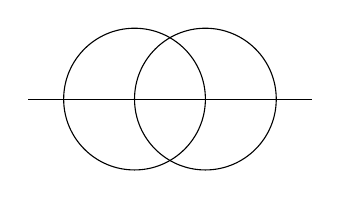
\begin{tikzpicture}[scale=0.9]
    \pgfmathsetmacro{\sqrttree}{sqrt(3)}
    \draw (-2,0) -- (2,0);
    \draw (-0.5,0) circle (1);
    \draw (0.5,0) circle (1);
    \end{tikzpicture}
\end{minipage}
\hfill
\begin{minipage}{0.22\textwidth} % Fourth diagram
    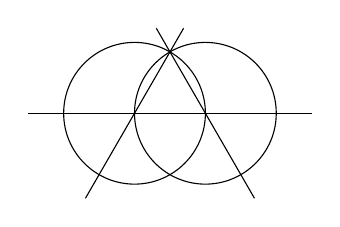
\begin{tikzpicture}[scale=0.9]
    \pgfmathsetmacro{\sqrttree}{sqrt(3)}
    \draw (-2,0) -- (2,0);
    \draw (-0.5,0) circle (1);
    \draw (0.5,0) circle (1);
    \draw (1.19282, -1.2) -- (-0.19282, 1.2);
    \draw (-1.19282, -1.2) -- (0.19282, 1.2);
    \end{tikzpicture}
\end{minipage}
\end{center}
\caption{Constructing an equilateral triangle by straight-edge and compass.}
\end{figure}
\noindent
The \emph{Elements} set the foundations for the study of geometry and remained the most important text on the subject for around 2000 years.

In the $17^\text{th}$ century, French mathematicians Ren\'{e} Descartes and Pierre de Fermat independently discovered \emph{coordinate geometry} \cite[Chapter 7]{Stillwell20}.
They realised that geometric points could be represented by $(x, y)$ coordinates.
Further, they described geometric shapes like lines and curves using algebraic equations.
This breakthrough meant that instead of relying on Euclid's constructive arguments, Descartes and Fermat could solve geometric problems using algebraic manipulation.
An example of a curve that Descartes studied is the \emph{folium} $X^3 + Y^3 = 3 XY$.

\begin{figure}[H]
\tikz{
    \draw[samples=200,domain=124:-35]plot(\x:{2*sin(\x)*cos(\x)/(sin(\x)^3+cos(\x)^3)})
}
\caption{The folium of Descartes, $X^3+Y^3+3XY$ \cite[p.\ 113]{Stillwell20}.}
\end{figure}


At the start of the $20^\text{th}$ century, mathematicians such as David Hilbert and Emmy Noether began developing the field of \emph{abstract algebra} \cite[\S 8.3]{Reid88}, and this would prove to have important implications for geometry.
One class of objects studied in abstract algebra are rings: structures where addition and multiplication are defined.
Familiar examples of rings include the integers $\ZZ$ and the ring of polynomials with real coefficients $\RR[X]$.

Hilbert realised rings could be used to study geometry.
The idea is that given a geometric space, one can associate a ring of functions on the space:
\begin{align*}
\begin{array}{c}
	\text{Geometric spaces} \\
	V
\end{array}
\rightsquigarrow
\begin{array}{c}
	\text{Rings} \\
	\Fun(V, \CC)
\end{array}
\end{align*}
Thus, geometry determines algebra.
The algebraic properties of $\Fun(V, \CC)$ encode geometric properties of the space $V$.
More remarkably, given a suitable ring $R$, one can determine a space $\Spec(R)$ that has $R$ as its ring of functions:
\begin{align*}
\begin{array}{c}
	\text{Geometric spaces} \\
	 \Spec(R)
\end{array}
\scalebox{-1}[1]{$\rightsquigarrow$}
\begin{array}{c}
	\text{Rings} \\
	R
\end{array}
\end{align*}
Thus, algebra determines geometry.
Hilbert's great insight, formalised by his famous theorem the \emph{Nullstellensatz}, was that studying geometry and algebra are equivalent.
The field that studies geometry using abstract algebra is called \emph{algebraic geometry}.

\subsection*{Algebraic geometry}
Algebraic geometry studies spaces called \emph{algebraic varieties} \cite{Reid88, Milne23, Hartshorne77}.
These are sets of solutions $(a_1, \ldots, a_n)$ in $\CC^n$ to polynomial equations
$$f_1(a_1, \ldots, a_n) = 0, \qquad \ldots, \qquad f_s(a_1, \ldots, a_n) = 0,$$
where $f_1, \ldots, f_s$ are  $n$-variable polynomials in $\CC[X_1, \ldots, X_n]$.
Familiar examples include the circle and the sphere.
Cubic curves and cones provide other examples.

\begin{figure}[H]
    \centering
    \begin{subfigure}[t]{0.23\textwidth}
        \centering
	\vspace{-0cm}
        
\begin{tikzpicture}
        \draw[ultra thick, myorange, samples=100, smooth] 
        plot[domain=0:360] ({cos(\x)}, {sin(\x)});
        \end{tikzpicture}
	  \vspace{0.2cm}
        \caption*{$X^2 + Y^2 = 1$}
    \end{subfigure}
    \hfill
    \begin{subfigure}[t]{0.23\textwidth}
        \centering
	\vspace*{-0.8cm}
        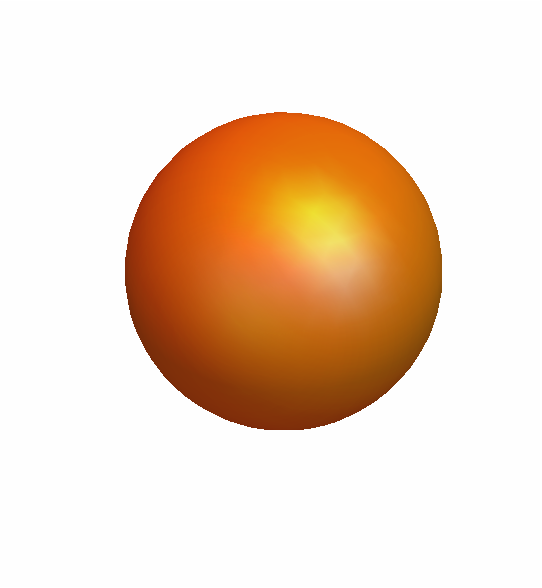
\includegraphics[width=\linewidth]{../images/orange_sphere}
	\vspace{-1.5cm}
        \caption*{$X^2 + Y^2 + Z^2 = 1$}
    \end{subfigure}
    \hfill
    \begin{subfigure}[t]{0.23\textwidth}
        \centering
        \vspace{-0cm} % Adjust vertical space if needed
        
\begin{tikzpicture}
          \draw[ultra thick, myorange, samples=100, smooth, domain=-2:0.65, variable=\x] 
            plot ({\x}, {sqrt((\x)^3 + 2*(\x)^2)});
          \draw[ultra thick, myorange, samples=100, smooth, domain=-2:0.65, variable=\x] 
            plot ({\x}, {-sqrt((\x)^3 + 2*(\x)^2)});
        \end{tikzpicture}
	 \vspace{0.1cm}
        \caption*{$Y^2 = X^3 + 2X^2$}
    \end{subfigure}
    \hfill
    \begin{subfigure}[t]{0.23\textwidth}
        \centering
        \vspace{-0.5cm} % Adjust vertical space for this subfigure
        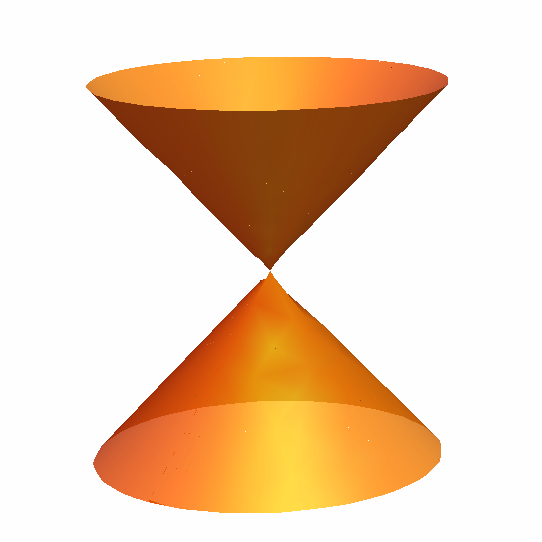
\includegraphics[width=0.8 \linewidth]{../images/orange_cone}
        \vspace{-0.2cm} % Adjust space below the image
        \caption*{$XY = Z^2$}
    \end{subfigure}
    \caption{Four examples of varieties.}
	\label{figure:fourvarieties}
\end{figure}

The third and fourth examples in Figure \ref{figure:fourvarieties} demonstrate that varieties may have \emph{singularities}: these are points where a variety is ``pinched".
The presence of singularities in varieties is one of the key differences between algebraic geometry and differential geometry.
In differential geometry, one studies smooth manifolds which have no singularities by definition.

Algebraic varieties are studied using polynomial functions in $\CC[X_1, \ldots, X_n]$.
Associated with a variety $V$ is the ideal of functions vanishing on $V$, which is denoted $\bI(V)$.
Using this, we define the \emph{coordinate ring} of $V$, which is the quotient ring
$$\CC[V] := \CC[X_1, \ldots, X_n] / \bI(V).$$
The ring $\CC[V]$ can be thought of as the ring of polynomial functions on $V$.
Thus, we have associated an algebraic object with the variety $V$.
The relationship between algebra and geometry is very close:
the ring $\CC[V]$ determines the variety $V$ up to isomorphism.
In this sense, the coordinate ring $\CC[V]$ is not just an algebraic shadow of $V$, but in fact, an equivalent object.

The equivalence between geometry and algebra means geometric properties have algebraic counterparts.
Below, we list key correspondences in the geometry--algebra dictionary.
These will be examined in Chapters \ref{chapter:algebraicsets} and \ref{chapter:affinevarieties}.

\begin{center}
\begin{tabular}{c | c}
	Geometry & Algebra \\
	\hline
	Points in $V$ & Maximal ideals of $\CC[V]$ \\
	Maps $V \to W$ & Homomorphisms $\CC[W] \to \CC[V]$ \\
	Irreducible varieties $V$ & Integral domains $\CC[V]$ \\
	Open subsets of $V$ & Localizations of $\CC[V]$ \\
	Tangent spaces $T_PV$ &  Zariski tangent spaces $(\frakm_P / \frakm_P^2)^*$
\end{tabular}
\end{center}

\hfill

Our discussion above introduces \emph{affine} algebraic varieties.
More general algebraic varieties can be constructed by glueing together affine varieties \cite[\S 5.0]{Reid88}, but we will not address these here.
In this thesis, all varieties are assumed to be affine.

\subsection*{Toric varieties}
In the $20^\text{th}$ century, algebraic geometers developed powerful tools for studying algebraic varieties, such as cohomology and homological algebra.
While these tools are abstract, they led to remarkable advances in the field.
Nevertheless, concrete examples of varieties remain essential to understand the subject \cite[p.\ ix]{Fulton93}.

\emph{Toric varieties} are a special class of varieties defined using elementary convex geometry, specifically using objects called \emph{convex cones}.
The cone defining a toric variety determines many of its properties, and can also often be used for explicit computations.
The explicit computations possible with toric varieties make them particularly valuable as examples in algebraic geometry \cite[p.\ ix]{Fulton93}.

In light of their computational tractability, toric varieties serve as important testing grounds for theories and conjectures in algebraic geometry.
For example, the Hodge conjecture---one of the million-dollar Millennium Prize Problems---has been proven for toric varieties, but is unresolved in general \cite{BM21}.

Toric varieties are named after the \emph{algebraic torus} $(\CC^\times)^n$.
This is an example of an \emph{algebraic group}: a variety which is also a group.
Toric varieties contain an algebraic torus as a dense open subset and admit an action of this torus (cf.\ \S \ref{section:thetorusaction}), so toric varieties can be viewed as generalisations of algebraic tori.

To illustrate the link between convex geometry and algebraic geometry in the theory of toric varieties, we present a simplified construction of a toric variety from a cone.
(Precise definitions will be given in Chapters \ref{chapter:convexgeometry} and \ref{chapter:affinetoricvarieties}.)
Consider the cone
$$\sigma = \Span_{\RR_{\ge 0}}\{e_1, -e_1+2e_2\},$$
where $\{e_1, e_2\}$ is the standard basis for $\RR^2$.
Using $\sigma$, we compute the \emph{dual cone}
$$\sigma^\vee = \Span_{\RR_{\ge 0}}\{e_2, 2e_1+ e_2\}.$$
To define a variety using $\sigma$ and $\sigma^\vee$, we construct a ring using these cones.
We first assign monomials $R^i S^j$ to integer-coordinate points $(i, j)$ in the vector space containing $\sigma^\vee$:
\begin{figure}[H]
    \centering
    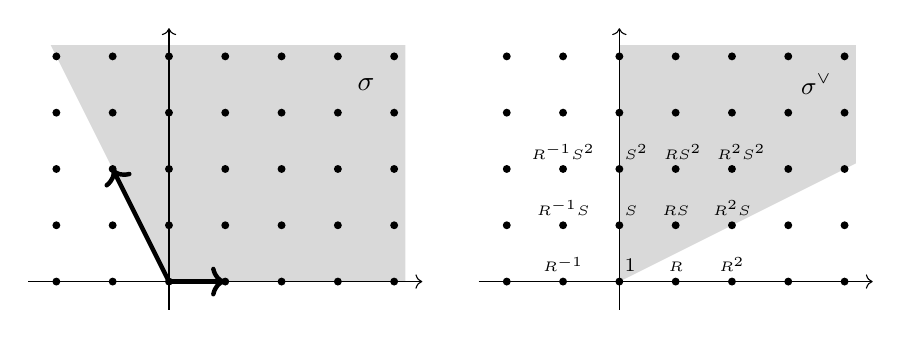
\begin{tikzpicture}[scale=1.43]
        % Left diagram
        \begin{scope}[shift={(-2,0)}]
            % Shaded area
            \fill[gray!30] (0,0) -- (-1.05, 2.1) -- (2.1,2.1) -- (2.1,0) -- cycle;
            
            % Axes
            \draw[->] (-1.25,0) -- (2.25,0);
            \draw[->] (0,-0.25) -- (0,2.25);
            
            % Lattice points
            \foreach \x in {-1,-0.5,0,0.5,1,1.5,2}
                \foreach \y in {0,0.5,1,1.5,2}
                    \fill (\x,\y) circle (1pt);

            % Vectors
            \draw[->, ultra thick] (0,0) -- (0.5,0);
            \draw[->, ultra thick] (0,0) -- (-0.5,1);
            \node at (1.75, 1.75) {$\sigma$};
        \end{scope}

        % Right diagram
        \begin{scope}[shift={(2,0)}]
            % Shaded area
            \fill[gray!30] (0,0) -- (0,2.1) -- (2.1,2.1) -- (2.1, 1.05) -- cycle;
            
            % Axes
            \draw[->] (-1.25,0) -- (2.25,0);
            \draw[->] (0,-0.25) -- (0,2.25);
            
            % Lattice points
            \foreach \x in {-1,-0.5,0,0.5,1,1.5,2}
                \foreach \y in {0,0.5,1,1.5,2} {
                    \fill (\x,\y) circle (1pt);
                }
                
			  % Labels
			  \node[anchor=south west] at (0, 0) {\!\!\! \scriptsize {$1$}};
  
			  \node[anchor=south ] at (-0.5, 0) {\tiny {$R^{-1}$}};
			  \node[anchor=south ] at (-0.5, 0.5) { \tiny {$R^{-1} S$}};
			  \node[anchor=south ] at (-0.5, 1) {\tiny {$R^{-1} S^2$}};

			  \node[anchor=south west] at (0, 0.5) {\!\!\! \tiny {$S$}};
			  \node[anchor=south west] at (0, 1) {\!\!\! \tiny {$S^2$}};

			  \node[anchor=south] at (0.5, 0) {\tiny {$R$}};
			  \node[anchor=south] at (0.5, 0.5) {\tiny {$R S$}};
			  \node[anchor=south] at (0.5, 1) {\, \tiny {$R S^2$}};

			  \node[anchor=south] at (1, 0) { \tiny {$R^2$}};
			  \node[anchor=south] at (1, 0.5) { \tiny {$R^2 S$}};
			  \node[anchor=south] at (1, 1) {\,\, \tiny {$R^2 S^2$}};

            % Vectors
            \node at (1.75, 1.75) {\small{$\sigma^\vee$}};
        \end{scope}
    \end{tikzpicture}
\end{figure}
\noindent
We create a ring $\CC[S_\sigma]$ using the monomials lying in the dual cone:
$$\CC[S_\sigma] = \CC[1, S, RS, R^2S, S^2,  RS^2, R^2S^2, \ldots] = \CC[S, R^2S, RS] \cong \CC[X, Y, Z]/(XY - Z^2).$$
Then $U_\sigma$, the toric variety determined by the cone $\sigma$, is defined to be the zero set of the polynomial relation in the ring:
$$XY = Z^2.$$

\subsection*{Geometric invariant theory}
Quotients are a key idea in all areas of mathematics.
In this thesis, we will study varieties arising as quotients of vector spaces by algebraic tori.
In general, it is a difficult problem to construct quotient spaces in geometry and topology with nice properties.
For example, consider $\GL_2(\CC)$ acting on $\CC^2$ by matrix multiplication.
There are two orbits for this action: $\{0\}$ and $\CC^2\setminus\{0\}$.
Using the quotient topology, the set of orbits is not Hausdorff, even though $\CC^2$ is.

Geometric invariant theory (henceforth abbreviated GIT) studies the problem of constructing quotients in algebraic geometry.
This theory was developed by David Mumford in the 1960s \cite{Mumford65}, though his work built on Hilbert's study of (classical) invariant theory.

To illustrate the relationship between Mumford and Hilbert's work, we outline the main goals of classical invariant theory.
Suppose a group $G$ acts on a vector space $V$, and write $\CC[V]$ for the ring of polynomial functions on $V$.
After choosing a basis for $V$, the ring $\CC[V]$ is identified with $\CC[X_1, \ldots, X_n]$.
The ring of invariants for the action is defined as
$$\CC[V]^G := \{f \in \CC[V] : f(g \cdot v) = f(v) \text{ for all } v \in V \text{ and all } g \in G\}.$$
Hilbert was interested in determining when the ring $\CC[V]^G$ is finitely generated \cite[Chapter 12]{FSR17}.
He proved that when $G$ is $\SL_n(\CC)$ acting on $V$ by a representation, $\CC[V]^G$ is finitely generated \cite{Hilbert90}.
Moreover, the invariant ring $\CC[V]^G$ is finitely generated for a large class of groups called \emph{reductive} groups---examples include $\GL_n(\CC)$, $\SL_n(\CC)$ and tori.
However, the invariant ring is not always finitely generated; in 1960, Masayoshi Nagata found an example where $\CC[V]^G$ fails to be finitely generated \cite{Nagata60}.

Mumford reformulated invariant theory in a geometric way.
He considered a group $G$ acting on any variety $V$.
If $\CC[V]$ is the coordinate ring of $V$, then the invariant ring $\CC[V]^G$ is defined as before.
Because invariant functions are constant on the orbits of the group action, we can think of $\CC[V]^G$ as the ring of polynomial functions on the space of orbits.
Mumford defined the affine GIT quotient $V \git G$ as the variety with $\CC[V]^G$ as its coordinate ring:
$$V \git G := \Spec(\CC[V]^G).$$
The question of when $\CC[V]^G$ is finitely generated remains important for GIT.
Mumford conjectured that $\CC[V]^G$ is finitely generated for \emph{geometrically reductive} groups, and this was proven by Nagata \cite[Chapter 13]{FSR17}.
If $\CC[V]^G$ is finitely generated by $m$ polynomials, then the GIT quotient $V \git G$ can be embedded in $\CC^m$.
When the ring is not finitely generated, however, the quotient $V \git G$ is not well-defined as a variety, as it would be ``infinite-dimensional".\footnote{Note $\Spec(\CC[V]^G)$ can still be studied as a scheme when $\CC[V]^G$ is not finitely generated, though we will not consider that case in this thesis. See \S \ref{section:themaximalspectrum} for the assumptions we make about coordinate rings of varieties.}

GIT is an important tool for constructing quotients in algebraic geometry.
However, this approach is not without drawbacks.
Firstly, the invariant ring $\CC[V]^G$ cannot always be computed explicitly.
Furthermore, points in $V \git G$ are not always in bijection with the orbits $V / G$, rather, points in the GIT quotient correspond to closed orbits (cf.\ Theorem \ref{theorem:gittheorem}).
Another drawback is that the GIT quotient $V \git G$ may be singular, even when $V$ is non-singular (cf.\ Example \ref{example:gitquotients}).

\subsection*{Goals and structure of this thesis}
In this thesis, we establish a connection between toric varieties and GIT quotients.
Specifically, the main goal of this thesis is to prove that when $V$ is a rational representation of a torus $T$, the GIT quotient $V \git T$ is an affine toric variety.
Our proof shows that the invariant ring $\CC[V]^T$ is finitely generated without appealing to general theorems about the finite generation of invariants.

To achieve our goal, we build up the preqrequisite theory of affine varieties and toric varieties.
We first explore the basic theory of algebraic sets and affine varieties in Chapter \ref{chapter:algebraicsets} and Chapter \ref{chapter:affinevarieties}, respectively.
Next, we delve into the convex geometry of cones in Chapter \ref{chapter:convexgeometry}.
Our understanding of varieties and convex geometry is applied in Chapter \ref{chapter:affinetoricvarieties} to study toric varieties.
Finally, in Chapter \ref{chapter:gitquotientsastoricvarieties}, we show $V \git T$ is a toric variety.

Each chapter in this thesis is shown with its main object of study in the diagram below.
An arrow from Chapter $i$ $\to$ Chapter $j$ indicates Chapter $i$ should be read before Chapter $j$.
\[\begin{tikzcd}
	\begin{array}{c} \text{Chapter \ref{chapter:algebraicsets}} \\ \text{Algebraic sets} \\ V \end{array} & \begin{array}{c} \text{Chapter \ref{chapter:affinevarieties}} \\ \text{Affine varieties} \\ \Spec(A) \end{array} \\
	\begin{array}{c} \text{Chapter \ref{chapter:convexgeometry}} \\ \text{Convex cones} \\ \sigma \end{array} & \begin{array}{c} \text{Chapter \ref{chapter:affinetoricvarieties}} \\ \text{Toric varieties} \\ U_\sigma \end{array} & \begin{array}{c} \text{Chapter \ref{chapter:gitquotientsastoricvarieties}} \\ \text{Torus quotients} \\ V \git T \end{array}
	\arrow[from=1-1, to=1-2]
	\arrow[from=1-2, to=2-2]
	\arrow[from=2-1, to=2-2]
	\arrow[from=2-2, to=2-3]
\end{tikzcd}\]
\noindent
We now detail the contents of each chapter.

In Chapter \ref{chapter:algebraicsets}, we introduce algebraic sets and develop the relationship between algebra and geometry.
We see how to associate ideals with algebraic sets, and conversely how to associate algebraic sets with ideals.
The relationship between ideals and algebraic sets becomes a bijection when we prove the Nullstellensatz.
We then consider maps on and functions between algebraic sets.
We relate direct products of algebraic sets to the algebraic operation of taking tensor products.
We conclude the chapter by considering open subsets of algebraic sets, and regular functions defined on these.

In Chapter \ref{chapter:affinevarieties}, we abstract our study of algebraic sets by defining affine varieties: these are algebraic sets without a preferred embedding in affine space.
Generalising our study of polynomial maps between algebraic sets, we investigate morphisms of affine varieties.
We also define tangent spaces and singular points of varieties, and characterise tangent spaces using ideals.

In Chapter \ref{chapter:convexgeometry}, we study the convex geometry we need to investigate toric varieties.
An important result we prove is that dualising a cone twice yields the original cone.
We focus on the types of cones used when defining toric varieties: these are polyhedral, rational, and strongly convex cones.
After defining these properties of convex geometry, we see how they have consequences for toric varieties in Chapter \ref{chapter:affinetoricvarieties}.

In Chapter \ref{chapter:affinetoricvarieties}, we develop the basic theory of toric varieties.
We define the semigroup algebra of a cone, then take the maximal spectrum to define a toric variety.
We investigate the different ways of viewing points in toric varieties from an algebraic perspective.
We prove that toric varieties admit an action of a torus which is a dense open subset.
We also see some ways how the convex geometry of the cone affects the geometry of the toric variety.
For example, there is a correspondence between faces of cones and certain subsets of varieties. 
Also, the cone determines whether the corresponding variety is singular.

In Chapter \ref{chapter:gitquotientsastoricvarieties}, we introduce algebraic groups and their actions.
This allows us to define the GIT quotient and state its main properties.
We will then be ready to show that $V \git T$ is a toric variety.
We compute the ring of invariants and then show this ring arises as the coordinate ring of a toric variety.
To conclude the thesis, we compute examples of the cones corresponding to $V \git T$.

\subsection*{Future directions}
This thesis only considers the affine theory of toric varieties and GIT quotients.
The theories of toric varieties and GIT can be studied in the general framework of algebraic varieties \cite{Fulton93, Mumford65}.
The main result of this thesis, that $V \git T$ is a toric variety, is also true in the general case (cf.\ \cite{Proudfoot05} or \cite[Chapter 12]{Dolgachev03}).
Further, under the correct assumptions the converse is also true, i.e., any toric variety can be understood as a quotient variety \cite[Chapter 5]{CLS11}.
These results provide interesting directions for future study.

This project originally set out to understand a particular torus quotient, namely, $\frakg \git T$.
Here, $T$ is a maximal torus in a connected complex reductive group $G$ with Lie algebra $\frakg$, and $T$ acts on $\frakg$ by the adjoint action.
In the course of investigating this quotient, we discovered the connection with toric varieties.
The last example of this thesis computes the cone of $\frakg \git T$ when $G = \GL_3(\CC)$.
A natural direction for future study is to investigate how the theory of toric varieties can help to understand $\frakg \git T$ in the general case.

\subsection*{Conventions}
In this thesis, $k$ is an algebraically closed field of characteristic zero, except in \S \ref{section:afffinespacealgsets} and \S \ref{section:ideal} where $k$ is an arbitrary field.
Coordinates of points are denoted using lowercase letters, for example, $(x, y) \in \AA^2$ or $(a_1, \ldots, a_n) \in \AA^n$.
Variables in rings are denoted using uppercase letters, for example, $X, Y, Z \in k[X, Y, Z]$ or $X_1, \ldots, X_n \in k[X_1, \ldots, X_n]$.






\newpage
\addtocontents{toc}{\protect\setcounter{tocdepth}{2}}
\section{Algebraic sets}\label{chapter:algebraicsets}
In this chapter, we introduce algebraic sets.
We begin by seeing how to associate algebraic sets with ideals in polynomial rings, and vice versa, in \S \ref{section:afffinespacealgsets} and \S \ref{section:ideal}.
Then, in \S \ref{section:thenullstellensatz}, we prove Hilbert's Nullstellensatz.
We investigate regular functions on algebraic sets, and polynomial maps between them in \S \ref{section:coordinateringsandpolynomialmaps}.
In \S \ref{section:productsofalgebraicsets}, we look at direct products of algebraic sets and how this is related to tensor products of coordinate rings.
The final section \S \ref{section:opensubsetsofalgebraicsets} studies open sets of algebraic sets and the regular functions defined on these.
Here, we have benefited from the exposition of \cite{Reid88} and \cite{Milne23}.




\subsection{Affine space and algebraic sets}\label{section:afffinespacealgsets}
In this section, we introduce affine space and define algebraic sets.
We also define the Zariski topology on algebraic sets.

Let $k$ be a field.
\emph{Affine space} over $k$, denoted $\AA^n_k$ or $\AA^n$, is the set 
$$\AA^n := \{(a_1, \ldots, a_n) : a_i \in k\}.$$
Elements of $\AA^n$ are called \emph{points}, and if $P = (a_1, \ldots, a_n) \in \AA^n$ is a point, then the $a_i$ are called the \emph{coordinates} of $P$.

Let $A$ denote the polynomial ring $k[X_1, \ldots, X_n]$.
We interpret a polynomial $f \in A$ as a function on $\AA^n$ by evaluating $f$ at the coordinates of a point $P = (a_1, \ldots, a_n)$, i.e., $f(P) := f(a_1, \ldots, a_n).$
This allows us to talk about the zeros of the polynomial, which is the set
$$\bV(f) := \{P \in \AA^n : f(P) = 0\} \subseteq \AA^n.$$
More generally, if $T \subseteq A$ is a set of polynomials, define
$$\bV(T) := \{P \in \AA^n : f(P) = 0 \text{ for all } f \in T\}.$$
A set $V \subseteq \AA^n$ is called \emph{algebraic} if $V = \bV(T)$ for some $T \subseteq A$.

Observe that if $\langle T \rangle \subseteq A$ is the ideal generated by $T$, then $\bV(T) = \bV(\langle T \rangle)$.
Moreover, Hilbert's famous Basis Theorem tells us all ideals of $A$ are finitely generated \cite[\S 3.6]{Reid95}.
Therefore, if $f_1, \ldots, f_r$ generate $\langle T \rangle$, then 
$$\bV(T) = \bV(\langle T \rangle) = \bV(\{f_1, \ldots, f_r\}).$$
We conclude that any algebraic set is the set of zeros of a finite number of polynomials.

\begin{example}\label{algsetex}
We list some examples of algebraic sets:
\begin{enumerate}
\item
$\AA^n$ and $\emptyset$ are algebraic, since $\AA^n = \bV(0)$ and $\emptyset = \bV(1)$.
Here, by $0$ and $1$ we mean the constant polynomials in $A$.

\item
Any line in $\AA^2$ has the form $\bV(aX+bY-c)$ for some $a, b, c \in k$, so lines are algebraic.

\item
The parabola $\bV(Y-X^2)$ is an algebraic set.

\item
The hyperbola $\bV(XY - 1)$ is an algebraic set.

\item
The twisted cubic $C = \{(t, t^2, t^3) \in \AA^3 : t \in k\}$ is an algebraic set.
We see this by noting $C = \bV(\{X^2 - Y, X^3 - Z\}).$

\item 
The curve $\bV(Y^2 - X^3)$ is algebraic, and it is an example of a so-called cuspidial cubic.

\item
We now give an example of a set which is not algebraic.
Suppose $k$ is infinite.
Let $S$ be an infinite subset of $\AA^1$ such that $S \ne \AA^1$.
Then $S$ is not of the form $\bV(\{f_1, \ldots, f_r\})$, since any $f_i \in k[X] \setminus \{0\}$ has finitely many roots.
In particular, $\AA^1 \setminus\{0\}$ is not an algebraic set in $\AA^1$.
\end{enumerate}
\end{example}

Our discussion above tells us that to study zero sets of polynomials, it suffices to study zero sets of ideals in $A$.
The map
$$\bV : \{\text{ideals } I \subseteq A\} \to \{\text{algebraic subsets } V \subseteq \AA^n\}, \qquad I \mapsto \bV(I),$$
is our first link between algebra and geometry.
The following result describes the behaviour of $\bV$:

\begin{proposition}\label{vproperties}
\begin{enumerate}
\item If $I \subseteq J$ are ideals, then $\bV(I) \supseteq \bV(J)$.
\item If $I_1$ and $I_2$ are ideals, then $\bV(I_1) \cup \bV(I_2) = \bV(I_1 I_2).$
\item If $\{I_\alpha\}_{\alpha \in \calA}$ is an arbitrary collection of ideals, then $\bigcap_{\alpha \in \calA} \bV(I_\alpha) = \bV\left(\sum_{\alpha \in \calA} I_\alpha\right)$.
\footnote{Here $\sum_{\alpha\in\calA} I_\alpha = \left\{\sum_{\alpha \in C} r_\alpha : C \text{ is a finite subset of } \calA, r_\alpha \in I_\alpha \right\}$ is the usual sum of ideals, which is defined even if $\calA$ is infinite.}
\end{enumerate}
\end{proposition}
\begin{proof}
(1) If $P \in \bV(J)$, then we have $f(P)=0$ for all $f \in I$, and $P \in \bV(I)$.

(2) Assume without loss of generality that $P \in \bV(I_1)$.
Then for all $f \in I_1$ and $g \in I_2$, we have $(fg)(P)=0$, implying all polynomials in $I_1 I_2$ vanish at $P$.
Conversely, if $P \in \bV(I_1 I_2)$ but $P \notin \bV(I_2)$, there is $g \in I_2$ with $g(P) \ne 0$.
But for any $f \in I_1$, there holds $(fg)(P)=0$, so $f(P)=0$.

(3) Suppose $P \in \bigcap_{\alpha \in \calA} \bV(I_\alpha)$.
Then for all $\alpha \in \calA$ and all $f_\alpha \in I_\alpha$, we have $f_\alpha(P) = 0$, implying every element of $\sum_{\alpha} I_\alpha$ vanishes at $P$.
Conversely, for each $\alpha$, part (1) tells us $\bV(I_\alpha) \supseteq \bV\left(\sum_{\alpha} I_\alpha\right)$ and so 
$\bigcap_{\alpha\in\calA} \bV(I_\alpha) \supseteq \bV\left(\sum_{\alpha\in\calA} I_\alpha\right).$
\end{proof}

Proposition \ref{vproperties} tells us arbitrary intersections and finite unions of algebraic sets are algebraic.
In Example \ref{algsetex}, we saw $\emptyset$ and $\AA^n$ are algebraic.
Together, these facts imply algebraic subsets of $\AA^n$ form the closed sets of a topology.
This topology is called the \emph{Zariski topology} on $\AA^n$.
We also endow algebraic sets $V$ with the subspace topology.
This is called the Zariski topology on $V$, and closed subsets of $V$ are refered to as algebraic subsets of $V$.

\begin{example}[The Zariski topology on $\AA^1$]\label{zariskia1}
Any non-constant polynomial in one variable has finitely many roots.
Then for any ideal $I \subseteq A$, $\bV(I)$ is either finite or all of $\AA^1$.
In other words, any closed set is either finite or $\AA^1$, so the Zariski topology on $\AA^1$ is the finite complement topology.
When $k$ is an infinite field, this topology is not Hausdorff; any two non-empty open sets have finite complements, so they necessarily intersect.
\end{example}

Example \ref{zariskia1} shows us that the Zariski topology is a very coarse toplogy, in the sense that open sets are large.
Nonetheless, the Zariski topology plays an important role in studying algebraic sets.





\subsection{The ideal of an algebraic set}\label{section:ideal}
The map $\bV$ gave us a map from ideals to algebraic subsets; this is our first link between algebra and geometry.
In this section, we consider another map $\bI$, which takes subsets of $\AA^n$ to ideals.
The map $\bI$ is defined as
$$\bI: \{\text{subsets } V \subseteq \AA^n\} \to \{\text{ideals } I \subseteq A\}, \quad V\mapsto \bI(V) := \{f \in A : f(P) = 0 \text{ for all } P \in V\}.$$
In other words, $\bI(V)$ is the ideal of functions vanishing on $V$.
We call $\bI(V)$ the \emph{ideal} of $V \subseteq \AA^n$.
The following result describes the behaviour of the map $\bI$:

\begin{proposition}\label{iproperties}
\begin{enumerate}
\item If $V \subseteq U \subseteq \AA^n$, then $\bI(V) \supseteq \bI(U)$.
\item If $V \subseteq \AA^n$, then $V \subseteq \bV(\bI(V))$, with equality if and only if $V$ is algebraic.
\item If $I \subseteq A$, then $I \subseteq \bI(\bV(I))$.
\end{enumerate}
\end{proposition}
\begin{proof}
(1) If $f \in \bI(U)$, then we have $f(P) = 0$ for all $P \in U$, so $f \in \bI(V)$.

(2) If $P \in V$, then $f(P) = 0$ for all $f \in \bI(V)$ and so $P \in \bV(\bI(V)).$
If $V = \bV(\bI(V))$, then $V$ is algebraic by definition.
Conversely, if $V = \bV(I)$ is algebraic, then the ideal of functions vanishing on $V$ will contain $I$.
Then $\bV(\bI(V)) \subseteq \bV(I) = V$ and $V = \bV(\bI(V))$.

(3) If $f \in I$, then for $P \in \bV(I)$, we have $f(P) = 0$, and so $f \in \bI(\bV(I)).$
\end{proof}

Proposition \ref{iproperties} begs a question: do $\bV$ and $\bI$ give a bijection between algebraic sets and ideals?
Unfortunately, the inclusion $I \subseteq \bI(\bV(I))$ may be strict, so $\bV$ are not $\bI$ are not always inverses of each other.
We give two examples of when this is the case:

\begin{example}\label{inclfails}
\begin{enumerate}
\item
Consider $I = (X^2) \subseteq k[X]$.
Then $\bV(I) = \{0\}$ but $\bI(\bV(I)) = (X) \supsetneq I.$

\item
Consider $I = (X^2+1)$ as an ideal in $A = \RR[X]$.
Then since $X^2+1$ never vanishes on $\AA^1_\RR$, $\bV(I) = \emptyset$, and it holds vacuously that $\bI(\bV(I)) = \RR[X] \supsetneq I.$
\end{enumerate}
\end{example}

Example \ref{inclfails} indicates two reasons why $I \subseteq \bI(\bV(I))$ may be a strict inclusion:
problems can occur when the equations defining an algebraic subset have ``unwanted multiplicities'', or when $k$ is not algebraically closed.
In \S \ref{section:thenullstellensatz}, we resolve these problems and make the maps $\bV$ and $\bI$ into bijections by considering an algebraically closed field, and a particular class of ideals called \emph{radical} ideals.

For the remainder of this section, we study the basic topological property of irreducibility, and explain how the map $\bI$ gives an algebraic characterisation of this property.
We say a non-empty subset $Y$ of a topological space $X$ is \emph{reducible} if $Y = Y_1 \cup Y_2$, where $Y_1$ and $Y_2$ are proper closed subsets of $Y$ \cite[Chapter I]{Hartshorne77}.
Otherwise, we say $Y$ is \emph{irreducible}.
In the context of the Zariski topology, an algebraic set $V \subseteq \AA^n$ is irreducible if it is not a union of proper algebraic subsets.

\begin{proposition}[{\cite[Proposition 1.1.12]{Geck13}}]\label{irreducibilityproposition}
Let $V \subseteq \AA^n$ be a non-empty algebraic set.
Then $V$ is irreducible if and only if $\bI(V)$ is prime.
\end{proposition}
\begin{proof}
Suppose $\bI(V)$ is not prime.
Then there exist $f_1, f_2 \notin \bI(V)$ such that $f_1 f_2 \in \bI(V)$.
Define $I_i := (\bI(V), f_i)$ for $i=1, 2$.
To see $V$ is reducible, we show that $V = \bV(I_1) \cup \bV(I_2)$, and that each $\bV(I_i)$ is a strict subset of $V$.
Since $I_i \supsetneq \bI(V)$, we have $\bV(I_i) \subsetneq \bV(\bI(V)) = V$, with strict inclusion because there is $P \in V$ with $f_i(P) \ne 0$.
Then we see $\bV(I_1) \cup \bV(I_2) \subseteq V$.
On the other hand, if $P \in V$, then $g(P) = 0$ for all $g \in \bI(V)$, and also $(f_1 f_2)(P) = 0$.
Thus, $f_1(P) = 0$ or $f_2(P)=0$, and $P \in \bV(I_1) \cup \bV(I_2)$.

Conversely, let $V = V_1 \cup V_2$ be reducible.
Since $V_1, V_2 \ne V$, we have $\bI(V_i) \supsetneq \bI(V)$, and there exists $f_i \in \bI(V_i) \setminus \bI(V)$ for $i=1,2$.
But $(f_1 f_2)(P) = 0$ for all $P \in V$, since if $P \in V_j$, then $f_j(P) = 0$.
Thus, $f_1 f_2 \in \bI(V)$ and $\bI(V)$ is not prime.
\end{proof}

\begin{example}
\begin{enumerate}
\item
Let $k$ be an infinite field.
It can be shown that any polynomial vanishing on all of $\AA^n$ must be the zero polynomial \cite[Example 1.1.13]{Geck13}.\footnote{Note that when $k$ is finite, non-zero polynomials can vanish on all of $\AA^n$.}
Proposition \ref{irreducibilityproposition} then implies that $\AA^n$ is irreducible, since $\bI(\AA^n) = \{0\}$ is a prime ideal.
We can also use Example \ref{zariskia1} to see $\AA^1$ is irreducible without appealing to Proposition \ref{irreducibilityproposition}.
Any proper closed subset of $\AA^1$ is finite, so $\AA^1$ cannot be a union of two proper closed subsets.

\item
Let $k$ be finite.
Since points are closed, a set is irreducible if and only if it is a singleton \cite[Example 1.1.13]{Geck13}.
In particular, $\AA^n$ is not irreducible in this case.

\item
An example of a reducible algebraic set is $V = \bV(XY) = \bV(X) \cup \bV(Y)$, the union of the $X$- and $Y$-axes.
Algebraically, we can see the reducibility of $V$ since $\bI(V) = (XY)$ is not prime
($X$ and $Y$ do not lie in $(XY)$, but $XY$ lies in $(XY)$).
\end{enumerate}
\end{example}





\subsection{The Nullstellensatz}\label{section:thenullstellensatz}
In this section and all sections henceforth, the field $k$ is assumed to be algebraically closed and have characteristic zero.
Our goal in this section is to upgrade the maps $\bV$ and $\bI$ to bijections between algebraic sets and radical ideals.
This is achieved by Hilbert's Nullstellensatz (Theorem \ref{null}).
To state and prove the theorem, we recall the following definition:

\begin{definition}
Let $I$ be an ideal of $A$.
The radical of $I$, denoted $\sqrt{I}$, is defined as
$$\sqrt{I} := \{f \in A : f^n \in I \text{ for some } n \in \ZZ_{> 0}\}.$$
We say an ideal is radical if $I = \sqrt{I}$.
\end{definition}

Observe that $I \subseteq \sqrt{I}$ for any ideal $I$.
We claim that prime ideals are radical.
If $I$ is prime and $f \in \sqrt{I}$, then $f^n \in I$ for some $n \in \ZZ_{> 0}$, which implies $f \in I$ since $I$ is prime.

To prove Theorem \ref{null}, we use the following fact from algebra:

\begin{theorem}[{\cite[\S 3.8]{Reid88}}]\label{hardfact}
Let $k$ be an infinite field, and $B = k[a_1, \ldots, a_n]$ a finitely generated $k$-algebra.
If $B$ is a field, then $B$ is algebraic over $k$, meaning every element of $B$ is the root of a polynomial in $k[X]$.
\end{theorem}

\begin{theorem}[Hilbert's Nullstellensatz {\cite[\S 3.10]{Reid88}}]\label{null}
Let $k$ be an algebraically closed field.
\begin{enumerate}
\item Every maximal ideal of $A = k[X_1, \ldots, X_n]$ is of the form $\frakm_P = (X_1 - a_1, \ldots, X_n - a_n)$ for some $P = (a_1, \ldots, a_n) \in \AA^n$.
\item If $I$ is a proper ideal of $A$, then $\bV(I) \ne \emptyset$.
\item For any ideal $I$, $\bI(\bV(I)) = \sqrt{I}$.
\end{enumerate}
\end{theorem}
\begin{proof}
(1) Let $\frakm \subseteq A$ be a maximal ideal.
Denote $K := k[X_1, \ldots, X_n] / \frakm$, and let $\varphi$ be the composition of the natural inclusion and quotient maps
$$\varphi \colon k \overset{\iota}{\hookrightarrow} k[X_1, \ldots, X_n] \overset{\pi}{\twoheadrightarrow} K.$$
Since $K$ is a field and finitely generated by $\pi(X_1), \ldots, \pi(X_n)$ as a $k$-algebra, Theorem \ref{hardfact} implies $K$ is algebraic over $k$.
Then $K $ is an algebraic field extension of $k$ and $\varphi$ is the inclusion of $k$ into $K$.
Since $k$ is algebraically closed, $\varphi$ is an isomorphism.
For each $i$, let $a_i := (\varphi^{-1}\circ\pi)(X_i)$, and set $P = (a_1, \ldots, a_n)$.
Then $\pi(X_i - a_i) = 0$ and $\frakm_P := (X_1 - a_1, \ldots, X_n - a_n) \subseteq \ker \pi = \frakm$.
But the map $k[X_1, \ldots, X_n] \to k$ defined by evaluation at $P$ induces the isomorphism $k[X_1, \ldots, X_n] / \frakm_P \cong k$.
Therefore $\frakm_P$ is maximal and $\frakm_P = \frakm$.

(2) Proper ideals are contained in some maximal ideal, so $I \subseteq \frakm_P$ for some $P \in \AA^n$.
Then $\bV(I) \supseteq \bV(\frakm_P) = \{P\}$ and $\bV(I) \ne \emptyset$.

(3) Let $I$ be any ideal in $A = k[X_1, \ldots, X_n]$ and let $f \in A$ be arbitary.
We introduce a new variable $Y$ and define the ideal
$$\tilde I := (I, f Y - 1) \subseteq k[X_1, \ldots, X_n, Y].$$
Intuitively, $\bV(\tilde I) \subseteq \AA^{n+1}$ is the set of points $P \in \bV(I)$ with $f(P) \ne 0$.
Specifically, if $Q = (a_1, \ldots, a_n, b) \in \bV(\tilde I)$, then $g(a_1, \ldots, a_n) = 0$ for all $g \in \bV(I)$
and $f(a_1, \ldots, a_n) \cdot b = 1$ (meaning $f(a_1, \ldots, a_n) \ne 0$).
If $f \in \bI(\bV(I))$ so $f(P) = 0$ for all $P \in \bV(I)$, then our previous discussion implies $\bV(\tilde I) = \emptyset$.
Thus, $\tilde I = A$ by part (2).
In particular, $1 \in \tilde I$, so there exist $f_i \in I$ and $g_0, g_i \in k[X_1, \ldots, X_n, Y]$ such that
$$1 = \sum g_i f_i + g_0 (f Y - 1)$$
as a polynomial in $k[X_1, \ldots, X_n, Y]$.
Evaluating the above expression at $Y = \frac{1}{f}$ yields
$$1 = \sum g_i(X_1, \ldots, X_n, 1/f) f_i(X_1, \ldots, X_n).$$
Each term in the sum is a rational function where the denominator is a power of $f$.
Thus there is some $N \in \ZZ_{> 0 }$ such that 
$$f^N = \sum f^N g_i (X_1, \ldots, X_n, 1/f) f_i(X_1,\ldots,X_n)$$
lies in $k[X_1, \ldots, X_n]$, and in particular, lies in $I$.
So $f \in \sqrt{I}$, proving $\sqrt{I} \supseteq \bI(\bV(I))$.
If $f \in \sqrt{I}$, then $f^N \in I \subseteq \bI(\bV(I))$ for some $N \in \ZZ_{> 0}$.
But then for any $P \in \bV(I)$, we must have $f(P) = 0$, so $f \in \bI(\bV(I))$.
\end{proof}

Combining the Nullstellensatz and Proposition \ref{irreducibilityproposition}, we get the following corollary:

\begin{corollary}\label{nullbijection}
The maps
$$\{\text{ideals } I \subseteq A\} \underset{\bI}{\overset{\bV}{\rightleftarrows}} \{\text{subsets } V \subseteq \AA^n\}$$
induce the following bijections:
$$
\begin{array}{c}
\{\text{radical ideals}\} \\
\{\text{prime ideals}\} \\
\{\text{maximal ideals}\} 
\end{array}
\begin{array}{c}
\longleftrightarrow \\
\longleftrightarrow \\
\longleftrightarrow  
\end{array}
\begin{array}{c}
\{\text{algebraic subsets}\}, \\
\{\text{irreducible subsets}\}, \\
\{\text{points}\} .
\end{array}
$$
\end{corollary}





\subsection{Coordinate rings and polynomial maps}\label{section:coordinateringsandpolynomialmaps}
In this section, we introduce the coordinate ring of an algebraic set and the related notion of a regular function.
We also define polynomial maps between algebraic sets, and see how these are related to $k$-algebra homomorphisms between coordinate rings.

Let $V \subseteq \AA^n$ be an algebraic set.
The \emph{coordinate ring} of $V$ is defined as
$$k[V] := k[X_1, \ldots, X_n] / \bI(V).$$
This is a finitely generated $k$-algebra.
In view of Proposition \ref{irreducibilityproposition}, $k[V]$ is an integral domain if and only if $V$ is irreducible.

The coordinate ring is also a \emph{reduced} $k$-algebra, meaning it has no non-zero nilpotent elements.
Since $\bI(V)$ is radical, this follows from the following general fact:

\begin{proposition}\label{reducedradical}
Let $I$ be an ideal in a ring $R$.
Then $R/I$ is reduced if and only if $I$ is radical.
\end{proposition}
\begin{proof}
The ring $R/I$ is reduced if and only if for all $n \in \ZZ_{> 0}$, $f^n + I = I$ implies $f + I = I$.
As a statement about elements instead of cosets, this says that $f^n \in I$ implies $ f \in I$, which is equivalent to $I = \sqrt{I}$.
\end{proof}

We say a function $\varphi \colon V \to k$ is \emph{regular} if there exists $f \in k[X_1, \ldots, X_n]$ such that $\varphi = \left. f \right|_V$.
Two polynomials $f, g \in k[X_1, \ldots, X_n]$ define the same regular function on $V$ if and only if $(f- g)(P) = 0$ for all $P \in V$, or equivalently, if $f + \bI(V) = g + \bI(V)$.
Thus, we identify the ring of regular functions on $V$ with $k[V]$.

Let $\pi : k[X_1, \ldots, X_n] \twoheadrightarrow k[V]$ be the quotient map.
The correspondence theorem from ring theory tells us that there is a bijection
\begin{align}\label{ringidealbijection}
\left\{
\begin{array}{c}
	\text{ideals of} \\
	k[V]=k[X_1,\ldots,X_n]/\bI(V)
\end{array}
\right\} \longleftrightarrow 
\left\{
\begin{array}{c}
	\text{ideals of } k[X_1, \ldots, X_n] \\
	\text{ containing } \bI(V)
\end{array}
\right\}.
\end{align}
In particular, any ideal of $k[V]$ is of the form $J/\bI(V)$, where $J$ is an ideal of $k[X_1, \ldots, X_n]$ containing $\bI(V)$.
If $J / \bI(V)$ is an ideal in $k[V]$, define
$$\bV(J/\bI(V)) := \{P \in V : f(P) = 0 \text{ for all } f \in J/\bI(V)\}.$$
If we think of elements of $J$ and $J/\bI(V)$ as functions on $V$, they are equal as sets (the quotient $J/\bI(V)$ identifies elements of $J$ if they define the same function).
It follows that
$$\bV(J/\bI(V)) = \bV(J).$$
The following result extends Corollary \ref{nullbijection} to a correspondence between ideals in $k[V]$ and subsets of $V$.

\begin{corollary}\label{corollary:coordinateringbijections}
We have the following bijections:
$$
\begin{array}{c}
\{\text{radical ideals in } k[V] \} \\
\{\text{prime ideals in } k[V] \} \\
\{\text{maximal ideals in } k[V] \} 
\end{array}
\begin{array}{c}
\longleftrightarrow \\
\longleftrightarrow \\
\longleftrightarrow  
\end{array}
\begin{array}{c}
\{\text{algebraic subsets of } V \}, \\
\{\text{irreducible subsets of } V\}, \\
\{\text{points of } V\} .
\end{array}
$$
\end{corollary}
\begin{proof}
The key idea of the proof is that whether an ideal is radical, prime or maximal is preserved by the bijection in Equation \ref{ringidealbijection}.
Algebraic sets $W$ contained in $V$ are in bijection with radical ideals $\bI(W)$ containing $\bI(V)$.
We have that
$$\frac{k[X_1, \ldots, X_n]}{\bI(W)} \cong \frac{k[X_1, \ldots, X_n]/\bI(V)}{\bI(W)/\bI(V)},$$
so in view of Proposition \ref{reducedradical}, $\bI(W)$ is radical if and only if $\bI(W)/\bI(V)$ is.
This establishes the first bijection, and the other two are analogous.
\end{proof}

We now turn our attention to polynomial maps between algebraic sets.
Let $V \subseteq \AA^n$ and $W \subseteq \AA^m$ be algebraic sets.
We write $X_1, \ldots, X_n$ for the coordinates on $\AA^n$ and $Y_1, \ldots, Y_m$ for the coordinates on $\AA^m$.

\begin{definition}
We say a map $\varphi : V \to W$ is polynomial if there exist $m$ polynomials $\varphi_1, \ldots, \varphi_m \in k[X_1, \ldots, X_n]$ such that
$$\varphi(P) = (\varphi_1(P), \ldots, \varphi_m(P))$$
for all $P \in V$.
\end{definition}

We claim a map $\varphi: V \to W$ is polynomial if and only if $Y_j \circ \varphi \in k[V]$ for all $j$.
If $\varphi$ is polynomial given by the components $\varphi_1, \ldots, \varphi_m$, then $Y_j \circ \varphi = \varphi_j$ is regular.
Conversely, if $\tilde \varphi_j := Y_j \circ \varphi \in k[V]$ and $\varphi_j \in k[X_1, \ldots, X_n]$ such that $\varphi_j \equiv \tilde \varphi_j \mod \bI(V)$, then $\varphi = (\varphi_1, \ldots, \varphi_m)$ and $\varphi$ is polynomial.

We also claim that the composition of polynomial maps is polynomial.
Let $U \subseteq \AA^l$ be algebraic, and let $\varphi: V \to W$ and $\psi : W \to U$ be polynomial maps.
If $\varphi_1, \ldots, \varphi_m$ and $\psi_1, \ldots, \psi_l$ are the components of $\varphi$ and $\psi$, respectively, the components of $\psi \circ \varphi : V \to U$ are
$$\psi_1(\varphi_1, \ldots, \varphi_m), \ldots, \psi_l(\varphi_1, \ldots, \varphi_m) \in k[X_1, \ldots, X_n].$$

We say a polynomial map $\varphi : V \to W$ is an isomorphism of algebraic sets if there exists a polynomial map $\psi: W \to V$ such that $\psi \circ \varphi = \mathrm{id}_V$ and $\varphi \circ \psi = \mathrm{id}_W$.

The following theorem relates polynomial maps to $k$-algebra homomorphisms of coordinate rings. 

\begin{theorem}\label{theorem:polynomialmapsandalgebrahomomorphisms}
Let $V \subseteq \AA^n$, $W \subseteq \AA^m$, and $U \subseteq \AA^l$ be algebraic sets.
\begin{enumerate}
\item
A polynomial map $\varphi:V \to W$ induces a $k$-algebra homomorphism $\varphi^*:k[W] \to k[V]$, given by $f \mapsto \varphi^*f := f \circ \varphi$.

\item
Any $k$-algebra homomorphism $\Phi:k[W] \to k[V]$ is of the form $\Phi = \varphi^*$ for a unique polynomial map $\varphi : V \to W$.

\item 
If $\varphi : V \to W$ and $\psi : W \to U$ are polynomial maps, then $(\psi \circ \varphi)^* = \varphi^* \circ \psi^*$.
\end{enumerate}
\end{theorem}

Note that together part (1) and (2) say that the map $\varphi \mapsto \varphi^*$ induces a bijection
\begin{align*}\label{polynomialmapkalghombijection}
\left\{
\begin{array}{c}
	\text{polynomial maps} \\
	V \to W
\end{array}
\right\} \longleftrightarrow 
\left\{
\begin{array}{c}
	k\text{-algebra homomorphisms} \\
	k[W] \to k[V]
\end{array}
\right\}.
\end{align*}
The map $\varphi^*$ is called the \emph{pullback} of $\varphi$.

\begin{proof}[Proof of Theorem \ref{theorem:polynomialmapsandalgebrahomomorphisms}]
(1) Since the composition of polynomial maps is polynomial, $\varphi^* f = f \circ \varphi \in k[V]$ for all $f \in k[W]$.
For $f, g \in k[W]$, we have:
\begin{align*}
	\varphi^*(f + g) &= (f+g)\circ\varphi = f\circ\varphi + g\circ\varphi = \varphi^*f + \varphi^*g,\\
	\varphi^*(fg) &= (fg)\circ\varphi = (f\circ\varphi)(g\circ\varphi) = (\varphi^* f)(\varphi^* g).
\end{align*}
Thus, $\varphi^*$ is a $k$-algebra homomorphism.

(2) We first show there exists a polynomial map $\varphi : V \to W$ with $\Phi = \varphi^*$.
If $g \in k[Y_1, \ldots, Y_m]$, we write $\overline{g}$ for the coset of $g$ in $k[W]$, for example, $\overline{Y_j} = Y_j + \bI(W)$.
Let $\varphi_i := \Phi(\overline{Y_i}) \in k[V]$ for $i=1,\ldots,m$, and define the polynomial map $\varphi:V \to \AA^m$ by
$$\varphi(P) = (\varphi_1(P), \ldots, \varphi_m(P)).$$
We need to show $\varphi(V) \subseteq W$ and $\varphi^* = \Phi$.
Since $\Phi$ is a homomorphism, we have for any $\overline{g} \in k[W]$ that
$$\Phi(\overline{g}) =\Phi(g(\overline{Y}_1, \ldots, \overline{Y}_m)) = g(\Phi(\overline{Y}_1), \ldots, \Phi(\overline{Y}_m)) = g(\varphi_1, \ldots, \varphi_m).$$
Then for any $P \in V$,
$$\Phi(\overline{g})(P) = g(\varphi_1(P), \ldots, \varphi_m(P)) = g(\varphi(P)).$$
When $g \in \bI(W)$, $\overline{g} = 0$ and the above equation implies that
$$g(\varphi(P)) = 0$$
for all $P \in V$, so $\varphi(V) \subseteq W$.
To see $\varphi^* = \Phi$, note that $\varphi^*(\overline{Y}_i) = \overline{Y}_i \circ \varphi = \varphi_i = \Phi(\overline{Y}_i).$
To show the uniqueness of $\varphi$, we prove the map $\varphi \mapsto \varphi^*$ is injective.
If $\varphi, \phi:V \to W$ are polynomial maps with components $\varphi_i$ and $\phi_i$, respectively, and $\varphi^*=\phi^*$, then for each $i$, 
$$\varphi_i = \varphi^*(\overline{Y}_i) = \phi^*(\overline{Y}_i) = \phi_i.$$
Therefore, $\varphi$ and $\phi$ have the same components and $\varphi=\phi$.

(3) For any $f \in k[U]$, we have
$$(\psi \circ \varphi)^* f = f \circ (\psi \circ \varphi) = (f \circ \psi) \circ \varphi = \varphi^*(\psi^* f),$$
so $(\psi \circ \varphi)^* = \varphi^* \circ \psi^*$.
\end{proof}

\begin{corollary}\label{isoofalgsetscoro}
A polynomial map $\varphi:V \to W$ is an isomorphism of algebraic sets if and only if $\varphi^*:k[W]\to k[V]$ is an isomorphism of $k$-algebras.
\end{corollary}

We now give examples of polynomial maps between algebraic sets and their pullbacks.

\begin{example}\label{example:polynomialmaps}
\begin{enumerate}
\item 
Let $C = \bV(\{X^2-Y, X^3-Z\})$ be the twisted cubic.
Consider the map $\varphi : \AA^1 \to C$ defined by $t \mapsto (t, t^2, t^3)$.
Note that $X \in k[C] = k[X, Y, Z]/(X^2-Y, X^3-Z)$ generates $k[C]$.
We write $k[T]$ for the coordinate ring of $\AA^1$.
Then the pullback $\varphi^* : k[C] \to k[T]$ is given by
$$X \mapsto X \circ \varphi = T.$$
Then $\varphi^*$ is a $k$-algebra isomorphism, and $C$ and $\AA^1$ are isomorphic as algebraic sets.

\item
Let $V = \bV(Y^2-X^3)\subseteq\AA^2$.
Consider $\varphi:\AA^1 \to V$ given by $t \mapsto (t^2, t^3)$.
Note $k[V] = k[X, Y]/(Y^2 - X^3)$ is generated by $X, Y \in k[V]$.
The pullback of $\varphi$ is $\varphi^*:k[V] \to k[T]$, given by
$$X \mapsto T^2, \qquad Y \mapsto T^3.$$
Then $\varphi^*(k[C]) = k[T^2, T^3] \ne k[T]$.

\item
Consider $\varphi:\AA^2 \to \AA^2$, given by $(x, y) \mapsto (xy, y)$.
The image is
$$\varphi(\AA^2) = \{(a_1,a_2) \in \AA^2 : a_1=a_2=0 \text{ or } a_2 \ne 0\}.$$
This set is not algebraic (since its Zariski closure is $\AA^2 \supsetneq \varphi(\AA^2)$), so the image of a polynomial map is not necessarily an algebraic set.
\end{enumerate}
\end{example}





\subsection{Products of algebraic sets}\label{section:productsofalgebraicsets}
Let $V_1 \subseteq \AA^n$ and $V_2 \subseteq \AA^m$ be algebraic sets.
In this section, we show how the direct product $V_1 \times V_2$ has the structure of an algebraic set.
Specifically, we show the coordinate ring of $V_1 \times V_2$ is isomorphic to the tensor product of $k$-algebras $k[V_1] \otimes_k k[V_2]$ (by Corollary \ref{isoofalgsetscoro}, to understand an algebraic set, it suffices to determine its coordinate ring).
Our approach using universal properties follows \cite[\S 1.0]{CLS11}, while \cite[\S 1.3.7]{Geck13} provides an alternative approach by computing the ideal of $V_1 \times V_2$.

We begin by describing the properties that the algebraic set $V_1 \times V_2$ should satisfying.
First, we want (polynomial) projection maps
$$\pi_1 : V_1 \times V_2 \to V_1, \qquad \text{and} \qquad \pi_2 : V_1 \times V_2 \to V_2.$$
Further, if $W$ is another algebraic set, specifying a polynomial map $W \to V_1 \times V_2$ should be equivalent to specifying two polynomial maps
$$\varphi_1 : W \to V_1, \qquad \text{and} \qquad \varphi_2 : W \to V_2.$$
More precisely, given $\varphi_1$ and $\varphi_2$ as above, there should exist a unique $\tilde \varphi$ such that the following diagram commutes
% https://q.uiver.app/#q=WzAsNCxbMCwwLCJWIl0sWzEsMCwiVlxcdGltZXMgVyJdLFsyLDAsIlciXSxbMSwxLCJVIl0sWzMsMCwiXFx2YXJwaGlfMSJdLFszLDIsIlxcdmFycGhpXzIiLDJdLFsxLDIsIlxccGlfMiJdLFsxLDAsIlxccGlfMSIsMl0sWzMsMSwiXFxleGlzdHMhIFxcdGlsZGVcXHZhcnBoaSIsMix7ImxhYmVsX3Bvc2l0aW9uIjo2MCwic3R5bGUiOnsiYm9keSI6eyJuYW1lIjoiZGFzaGVkIn19fV1d
\[\begin{tikzcd}
	V_1 & {V_1 \times V_2} & V_2 \\
	& W
	\arrow["{\pi_1}"', from=1-2, to=1-1]
	\arrow["{\pi_2}", from=1-2, to=1-3]
	\arrow["{\varphi_1}", from=2-2, to=1-1]
	\arrow["{\exists! \tilde\varphi}"'{pos=0.6}, dashed, from=2-2, to=1-2]
	\arrow["{\varphi_2}"', from=2-2, to=1-3]
\end{tikzcd}\]
\noindent
The above characterisation of $V_1 \times V_2$, dualised to a statement about coordinate rings, says that there should exist homomorphisms
$$\iota_1 : k[V_1] \to k[V_1 \times V_2], \qquad \text{and} \qquad \iota_2 : k[V_2] \to k[V_1 \times V_2],$$
such that for every pair of $k$-algebra homomorphisms
$$\alpha_1 : k[V_1] \to k[W], \qquad \text{and} \qquad \alpha_2 : k[V_2] \to k[W],$$
there exists a unique $k$-algebra homomorphism $\tilde \alpha$ making the following diagram commute
% https://q.uiver.app/#q=WzAsNCxbMSwwLCJBIl0sWzAsMCwia1tWXSJdLFsyLDAsImtbV10iXSxbMSwxLCJrW1VdIl0sWzEsMywiXFxhbHBoYV8xIiwyXSxbMiwzLCJcXGFscGhhXzIiXSxbMSwwLCJcXGlvdGFfMSJdLFsyLDAsIlxcaW90YV8yIiwyXSxbMCwzLCJcXGV4aXN0cyEgXFx0aWxkZSBcXGFscGhhIiwwLHsibGFiZWxfcG9zaXRpb24iOjMwLCJzdHlsZSI6eyJib2R5Ijp7Im5hbWUiOiJkYXNoZWQifX19XV0=
\[\begin{tikzcd}
	{k[V_1]} & k[V_1 \times V_2] & {k[V_2]} \\
	& {k[W]}
	\arrow["{\iota_1}", from=1-1, to=1-2]
	\arrow["{\alpha_1}"', from=1-1, to=2-2]
	\arrow["{\exists! \tilde \alpha}"{pos=0.3}, dashed, from=1-2, to=2-2]
	\arrow["{\iota_2}"', from=1-3, to=1-2]
	\arrow["{\alpha_2}", from=1-3, to=2-2]
\end{tikzcd}\]
\noindent
This universal property of $k[V_1 \times V_2]$ implies it is isomorphic to the tensor product of $k$-algebras $k[V_1] \otimes_k k[V_2]$.

We now explain how $k[V_1] \otimes_k k[V_2]$ is defined, following \cite[Chapter 1, e]{Milne23}.
The underlying vector space of $k[V_1] \otimes_k k[V_2]$ is the tensor product of the vector spaces $k[V_1]$ and $k[V_2]$.
The multiplication is given on pure tensors by
$$(f \otimes g)(f' \otimes g') := (f f') \otimes (g g').$$
We have a homomorphism $k \to k[V_1] \otimes_k k[V_2]$ given by $1 \mapsto 1 \otimes 1$ which makes $k[V_1] \otimes_k k[V_2]$ a $k$-algebra.
The homomorphisms $\iota_1 : k[V_1] \to k[V_1] \otimes_k k[V_2]$ and $\iota_2 : k[V_2] \to k[V_1] \otimes_k k[V_2]$ are given by
$$f \mapsto f \otimes 1, \qquad \text{and} \qquad g \mapsto 1 \otimes g,$$
respectively.

To realise $k[V_1] \otimes_k k[V_2]$ as an algebra of functions on $V_1 \times V_2$, one computes
$$(f \otimes g)(P, Q) := f(P)g(Q),$$
for $f \in k[V_1]$, $g \in k[V_2]$ and $(P, Q) \in V_1 \times V_2$ \cite[Remark 1.58]{Milne23}.

We now give a basic example of the tensor product of two $k$-algebras, following \cite[Example 1.57]{Milne23}.

\begin{example}
Consider the affine spaces $V_1 = \AA^n$ and $V_2 = \AA^m$, and their coordinate rings $k[V_1] = k[X_1, \ldots, X_n]$ and $k[V_2] = k[Y_1, \ldots, Y_m]$.
Then the tensor product $k[V_1] \otimes_k k[V_2]$ is isomorphic to $k[X_1, \ldots, X_n, Y_1, \ldots, Y_m]$.
The homomorphisms $\iota_1 : k[V_1] \to k[X_1, \ldots, X_n, Y_1, \ldots, Y_m]$ and $\iota_2 : k[V_2] \to k[X_1, \ldots, X_n, Y_1, \ldots, Y_m]$ are given by the obvious inclusions.
In terms of the constructive definition of tensor products, the isomorphism is
$$k[V_1] \otimes_k k[V_2] \to k[X_1, \ldots, X_n, Y_1, \ldots, Y_m], \qquad f \otimes g \mapsto fg.$$
Geometrically, this says that $\AA^n \times \AA^m$ is isomorphic to $\AA^{n+m}$, as expected.
\end{example}



\subsection{Open subsets of algebraic sets}\label{section:opensubsetsofalgebraicsets}
In this section, we study principal open subsets of algebraic sets.
In particular, we show these are algebraic sets in their own right, and describe their coordinate ring using localization.
We conclude by defining regular functions on open subsets of an algebraic set.

Let $V \subseteq \AA^n$ be an algebraic set and $f \in k[V]$ a polynomial function on $V$.
Then the set
$$V_f := \{P \in V : f(P) \ne 0\}$$
is an open subset of $V$, since its complement (the zero set of $f$) is algebraic.
It turns out that the set $\{V_f : f \in k[V]\}$ is a basis for the Zariski topology on $V$:

\begin{proposition}[{\cite[Proposition 2.37]{Milne23}}]
The set $\{V_f : f \in k[V]\}$ is a basis for the Zariski topology on $V$.
Specifically, every open set is a finite union of the form $\bigcup V_f$.
\end{proposition}
\begin{proof}
Every open set $U \subseteq V$ is the complement of $\bV(J)$ for some ideal $J$ of $k[V]$.
If $J$ is generated by $f_1, \ldots, f_m$, then $U = \bigcup V_{f_i}.$
\end{proof}

In light of the proposition, sets of the form $V_f$ are called \emph{principal open subsets} of $V$.

We now explain how we can think of a principal open subset $V_f$ as an algebraic set in its own right.
Suppose $\bI(V)$ is generated by $f_1, \ldots, f_m \in k[X_1, \ldots, X_n]$.
Let $g \in k[X_1, \ldots, X_n]$ be a coset representative for $f$ in $k[V] = k[X_1, \ldots, X_n]/\bI(V)$.
Writing $k[X_1, \ldots, X_n, Y]$ for the coordinate ring of $k^n \times k$, we define a new algebraic set $W \subseteq k^n \times k$ by 
$$W:=\bV(f_1, \ldots, f_m, g Y - 1).$$
A point $(x_1, \ldots, x_n, y) \in W$ satisfies $f_i(x_1, \ldots, x_n) = 0$ for all $i$, and  $g(x_1, \ldots, x_n) = \frac{1}{y} \ne 0$.
It follows that the projection $k^n \times k \to k^n$ identifies $V_f$ with the algebraic set $W$.

It is natural to ask what the coordinate ring of $V_f$ is.
The coordinate ring of the algebraic set $W$ described above is $k[X_1,\ldots, X_n,Y]/(f_1, \ldots, f_m, gY-1).$
This is one description of $k[V_f]$, but it can be constructed in a way that does not require choosing generators $f_1, \ldots, f_m$.
We will see that $k[V_f]$ is a certain ring of fractions of $k[V]$.

Recall that when $A$ is an integral domain, one can construct the field of fractions $\Frac(A)$.
The construction of a ring of fractions is a generalisation where $A$ is not required to be an integral domain and a subset of elements of $A$ are inverted.
We now define rings of fractions, following \cite[\S 3]{AM16}.

Let $A$ be any commutative ring with identity.
Let $S$ be a multiplicatively closed subset of $A$, meaning a subset containing the identity which is closed under multiplication.
We define a relation on $A \times S$ by declaring $(a, s) \sim (b, t)$ if there exists $u \in S$ such that $u(at - bs)=0$.
It is clear that $\sim$ is reflexive and symmetric, and it is straightforward to show it is transitive \cite[\S 3]{AM16}.
The equivalence class of $(a,s)$ is denoted $\frac{a}{s}$, and the set of equivalence classes is denoted $S^{-1}A$.
Addition and multiplication in $S^{-1}A$ is defined in the usual way for fractions:
$$\frac{a}{s}+\frac{b}{t} := \frac{at+bs}{st}, \qquad \frac{a}{s}\cdot\frac{b}{t} := \frac{ab}{st}.$$
A routine verification shows that these operations are well-defined and make $S^{-1}A$ into a commutative ring with identity \cite[\S 3]{AM16}.
There is a ring homomorphism $A\to S^{-1}A$ given by $a \mapsto \frac{a}{1}$.
Then $a\in A$ is in the kernel of this map if $\frac{a}{1}=\frac{0}{1}$ in $S^{-1}A$, which is equivalent to the existence of $u\in S$ such that $u a = 0$.

We now consider two examples: the first relates rings of fractions to the field of fractions of an integral domain, and the second will be important for describing $k[V_f]$.

\begin{example}
\begin{enumerate}
\item
Let $A$ be an integral domain and $S = A \setminus \{0\}$.
Then $S^{-1}A$ can be identified with the field of fractions $\Frac(A)$.
More generally, if $T$ is any multiplicatively closed subset of $A$, $T^{-1}A$ can be identified with the subring $\{\frac{a}{t} : a\in A, t \in T\}$ of $\Frac(A)$.

\item
Let $h \in A$ and choose $S = \{1, h, h^2, \ldots\}$.
In this case, $S^{-1}A$ is denoted $A_h$.
Every element of $A_h$ can be written $\frac{a}{h^m}$ for some $a \in A$ and $m \in \ZZ_{\ge 0}$.
We have that $\frac{a}{h^m} = \frac{b}{h^n}$ if and only if $h^N (ah^n - b h^m)=0$ for some $N \in \ZZ_{\ge 0}$.
This implies that if $h$ is nilpotent, then there is one equivalence class and $A_h = \{0\}$.
If $A$ is an integral domain and $h \ne 0$, the previous example tells us $A_h$ can be identified with the subring $\{\frac{a}{h^n} : a \in A, n \in \ZZ_{\ge 0}\}$ of $\Frac(A)$.
The ring $A_h$ is called the \emph{localization} of $A$ at $h$, and the map $A \to A_h$ given by $a \mapsto \frac{a}{1}$ is called the \emph{localization homomorphism}.
\end{enumerate}
\end{example}

The following lemma realises $A_h$ as a quotient ring:

\begin{lemma}[{\cite[Lemma 1.13]{Milne23}}]\label{lemma:localizationisomorphism}
For every ring $A$ and $h \in A$,
$$A[Y]/(hY-1) \cong A_h.$$
\end{lemma}

The lemma implies that
$$k[V_f] \cong k[V]_f.$$
This follows from our previous discussion, where we saw that if $f_1, \ldots, f_m$ generate $\bI(V)$ and $f = g + \bI(V)$, then the coordinate ring of $V_f$ is isomorphic to
$$k[X_1,\ldots, X_n,Y]/(f_1, \ldots, f_m, gY-1) \cong (k[V][Y])/(fY-1) \cong k[V]_f.$$
Therefore, the ring of fractions $k[V]_f$ allows us to understand the coordinate ring of $V_f$ without choosing generators for $k[V]$.

An important example of an algebraic set which arises as a principal open subset of $\AA^n$ is the algebraic torus
$$(k^\times)^n := \{(x_1, \ldots, x_n) \in k^n : x_i \ne 0\}.$$
Observe that $(k^\times)^n = \AA^n \setminus \bV(X_1 \cdots X_n)$.
Then, the coordinate ring of $(k^\times)^n$ is 
$$k[X_1, \ldots, X_n]_{X_1 \cdots X_n} = k[X_1, X_1^{-1}, \ldots, X_n, X_n^{-1}],$$
the ring of Laurent polynomials.

The following proposition describes the relationship between ideals in $A$ and ideals in a ring of fractions $S^{-1} A$.
This will be important for Proposition \ref{proposition:localizationembedding}, when we investigate open subsets of affine varieties.

\begin{proposition}[{\cite[Proposition 1.14]{Milne23}}]\label{proposition:localizationideals}
Let $S$ be a multiplicatively closed subset of a ring $A$.
The map
$$\frakp \mapsto (S^{-1}A) \frakp$$
is a bijection between the set of prime ideals of $A$ disjoint from $S$, and the set of prime ideals of $S^{-1}A$.
\end{proposition}

Note that the map $\frakp \mapsto (S^{-1}A) \frakp$ preserves inclusion, so it is a bijection between maximal ideals of $A$ disjoint from $S$ and maximal ideals of $S^{-1}A$.

We now define regular functions on open subsets of algebraic sets.
These are functions we use to study algebraic sets which are a broader class than polynomial functions.

\begin{definition}
Let $U$ be an open subset of an algebraic set $V$.
A function $f : U \to k$ is called regular at $P \in U$ if there exist $g, h \in k[V]$ with $h(P)\ne 0$ such that $f = \frac{g}{h}$ on some neighbourhood of $P$.
A function $f:U\to k$ is called regular if it is regular at every $P \in U$.
\end{definition}

It can be shown when $U = V$, the only regular functions on $U$ are the polynomial functions on $V$ \cite[Proposition 3.11]{Milne23}.

We now consider an example of a regular function.

\begin{example}
Consider $V = \bV(X_1 X_4 - X_2 X_3) \subseteq \AA^4$ and the open subset
$$U = V \setminus \bV(X_2, X_4) = \{(x_1, \ldots, x_4) \in V : x_2 \ne 0 \text{ or } x_4 \ne 0\}.$$
Define the function
$$\varphi : U \to k, \qquad
(x_1, \ldots, x_4) \mapsto 
\begin{cases} 
	\frac{x_1}{x_2} & \text{if } x_2 \ne 0, \\ 
	\frac{x_3}{x_4} & \text{if } x_4 \ne 0. 
\end{cases}$$
It is well-defined since $\frac{x_1}{x_2} = \frac{x_3}{x_4}$ if $x_2 \ne 0$ and $x_4 \ne 0$, and regular since it is locally given by quotients of polynomials.
\end{example}

We write $\calO_V(U)$ for the $k$-algebra of regular functions $U \to k$.
The following proposition describes some properties of the assignment $U \mapsto \calO_V(U)$.
These properties motivate our discussion of sheaves in the next chapter.

\begin{proposition}\label{sheafprop}
\begin{enumerate}
\item
$\calO_V(U)$ is a $k$-subalgebra of $\Fun(U, k)$, the $k$-algebra of all $k$-valued functions on $U$.
\item
If $f \in \calO_V(U)$ and $U'\subseteq U$ is an open subset, then $\left. f \right|_{U'} \in \calO_V(U')$.
\item
If $\{U_i\}$ is an open cover of $U$ and $f_i \in \calO_V(U_i)$ satisfy $\left. f_i \right|_{U_i \cap U_j} = \left. f_j \right|_{U_i \cap U_j}$ for all $i$ and $j$, then the unique function $f : U \to k$ such that $\left. f \right|_{U_i} = f_i$ lies in $\calO_V(U)$.
\end{enumerate}
\end{proposition}
\begin{proof}
\begin{enumerate}
\item
It is clear that a constant function is regular.
Let $f_1$ and $f_2$ be regular on $U$ and fix a point $P \in U$.
Then, there exists a neighbourhood $W$ of $P$ and $g_1, g_2, h_1, h_2 \in k[V]$ such that $f_i = \frac{g_i}{h_i}$ on $W$.
Therefore, $f_1 + f_2 = \frac{g_1 h_2 + g_2 h_1}{h_1 h_2}$ and $f_1 f_2 = \frac{g_1 g_2}{h_1 h_2}$ on $W$.

\item
For any $P \in U'$, $f$ is regular at $P \in U$, so $\left. f \right|_{U'}$ is regular.

\item
To see $f \in \calO_V(U)$, note that if $P \in U$, then $P\in U_i$ for some $i$, and $f$ is regular at $P$ since it is locally equal to $f_i$.
\end{enumerate}
\end{proof}











\newpage
\section{Affine varieties}\label{chapter:affinevarieties}
In this chapter, we define and study affine varieties---these are spaces which `look like' algebraic sets, but defined without needing to be embedded in an affine space.
This definition is necessary because we usually want to study spaces without an ambient space.
In particular, when we study toric varieties and GIT quotients in later chapters, we will need to define a space by prescribing its coordinate ring.
This is easily achieved in the context of affine varieties by the taking the maximal spectrum of the desired coordinate ring.

We start by defining sheaves, which is an assignment of a set of functions to open sets in a topological space---this is an abstraction of looking at the regular functions defined on an open subset of an algebraic set.
Affine varieties can then be defined as a topological space with a sheaf that looks like an algebraic set.
For the rest of the chapter, we study morphisms and tangent spaces of varieties.






\subsection{Sheaves and their morphisms}\label{varietiessection}
Proposition \ref{sheafprop} alludes to an important object appearing in many areas of mathematics, called a sheaf.
We will use the notion of a sheaf of $k$-algebras to define affine varieties, opting to avoid the most general definition of sheaves appearing in the literatue (cf.\ {\cite[Chapter II, \S 1]{Hartshorne77}}).

\begin{definition}[{\cite[Chapter 3, a]{Milne23}}]\label{sheafdef}
Let $V$ be a topological space and $k$ a field.
Suppose that for every open subset $U \subseteq V$, we have a set $\calO_V(U)$ of functions $U \to k$.
We say the assignment $U \mapsto \calO_V(U)$ is a sheaf of $k$-algebras if the following hold for every open subset $U \subseteq V$:
\begin{enumerate}
\item
$\calO_V(U)$ is a $k$-subalgebra of $\Fun(U, k)$, the $k$-algebra of all $k$-valued functions on $U$;
\item
if $f \in \calO_V(U)$ and $U'\subseteq U$ is an open subset, then $\left. f \right|_{U'} \in \calO_V(U')$; and,
\item
if $\{U_i\}$ is an open cover of $U$ and $f_i \in \calO_V(U_i)$ satisfy $\left. f_i \right|_{U_i \cap U_j} = \left. f_j \right|_{U_i \cap U_j}$ for all $i$ and $j$, then the unique function $f : U \to k$ such that $\left. f \right|_{U_i} = f_i$ lies in $\calO_V(U)$.
\end{enumerate}
A pair $(V, \calO_V)$ consisting of a topological space $V$ and a sheaf of $k$-algebras on $V$ is called a $k$-ringed space, or a ringed space when $k$ is understood.
The $k$-algebra $\calO_V(U)$ is sometimes denoted $\Gamma(U, \calO_V)$, and its elements are called the sections of $\calO_V$ over $U$.
\end{definition}

Proposition \ref{sheafprop} says that for an algebraic set $V$, the assignment sending an open subset $U \subseteq V$ to its ring of regular functions $\calO_V(U)$ is a sheaf of $k$-algebras.
This sheaf is called the \emph{structure sheaf} of $V$.
As we will see, structure sheaves are one of the main tools we use to define and study varieties.
To further illustrate the definition of a sheaf, we give further examples as well as a non-example:

\begin{example}
\begin{enumerate}
\item Let $V$ be any topological space.
For any open set $U$, let $\calO_V(U)$ be the set of continuous functions $U \to \RR$.
It is clear $\calO_V$ satisfies condition (1) in Definition \ref{sheafdef}.
Conditions (2) and (3) hold since continuity is a \emph{local property}, i.e., $f : U \to \RR$ is continuous if and only if for all open covers $\{U_i\}$ of $U$, $\left. f \right|_{U_i}$ is continuous for all $i$. Thus $\calO_V$ is a sheaf of $\RR$-algebras.
\item Consider $V = \RR$ with the standard topology, and let $\calO_V(U)$ be the set of differentiable functions $U \to \RR$.
Differentiability is a local property, so $\calO_V$ is a sheaf of $\RR$-algebras.
\item If $(V, \calO_V)$ is a ringed space and $U$ is an open subset of $V$, then $\left. \calO_V \right|_U$, the restriction of $\calO_V$ to open subsets of $U$, is a sheaf on $U$.
\item Consider $V = \RR$ with the standard topology, and let $\calO_V(U)$ be the set of bounded functions $U \to \RR$.
This does not define a sheaf since condition (3) of Definition \ref{sheafdef} does not hold;
let $\{U_i\}$ be the open cover of $\RR$ given by $U_i:=(-i, i)$ and observe that $f_i(x):=x$ lies in $\calO_V(U_i)$ for each $i$ but $f(x) = x$ does not lie in $\calO_V(\RR)$.
This fails to be a sheaf because boundedness is not a local property.
\end{enumerate}
\end{example}

Having defined sheaves and ringed spaces, we need to define the structure-preserving maps between them; these are called morphisms of ringed spaces.
Given a map $\varphi : V \to W$ between topological spaces, any function $f : W \to k$ on $W$ defines a function $\varphi^* f := f \circ \varphi : V \to k$ on $V$.
We call $\varphi^* f$ the \emph{pullback} of $f$ by $\varphi$.
Morphisms of ringed spaces are continuous maps that ensure the pullback of any function in the sheaf on $W$ lies in the sheaf on $V$.
The precise definition is as follows:

\begin{definition}\label{definition:morphismringedspace}
Let $(V, \calO_V)$ and $(W, \calO_W)$ be ringed spaces.
A morphism of ringed spaces $\varphi : V \to W$ is a map such that
\begin{enumerate}
\item 
$\varphi$ is continuous, and
\item
for all open subsets $U \subseteq W$, if $f \in \calO_W(U)$, then $\varphi^* f = f\circ\varphi \in \calO_V(\varphi^{-1}(U))$.
\end{enumerate}
\end{definition}

Observe that if $\varphi : V \to W$ is a morphism, then the map $\varphi^* : \calO_W(W) \to \calO_V(V)$ defined by $f \mapsto \varphi^* f$ is a homomorphism of $k$-algebras.
Thus, morphisms respect the algebraic structure of the $k$-algebras $\calO_W(W)$ and $\calO_V(V)$.

\begin{example}
\begin{enumerate}
\item
Consider any topological spaces $V$ and $W$ with their sheaves of continuous real-valued functions.
Any continuous map $V \to W$ is a morphism. The second condition in Definition \ref{definition:morphismringedspace} holds because composition preserves continuity.

\item
If $(V, \calO_V)$ is a ringed space and $U$ is an open subset of $V$, the inclusion $U \hookrightarrow V$ is a morphism between the ringed spaces $(U, \left. \calO_V\right|_U)$ and $(V, \calO_V)$.
\end{enumerate}
\end{example}

We say that a morphism of ringed spaces is an \emph{isomorphism} if it is bijective and its inverse is also a morphism.
Then isomorphisms are in particular homeomorphisms.





\subsection{The definition of varieties}
Having defined ringed spaces, we can now define affine varieties.
In Chapter \ref{chapter:algebraicsets}, we studied algebraic sets embedded in an ambient affine space.
Roughly speaking, an affine variety is an algebraic set, defined without choosing an embedding into affine space.
This is analogous to how a smooth manifold is defined intrinsically as a topological space, without reference to an ambient Euclidean space.
The following definition makes this precise using ringed spaces:

\begin{definition}
An affine variety over $k$ is a $k$-ringed space isomorphic to one of the form $(V, \calO_V)$ for some algebraic set $V \subseteq \AA^n$.
\end{definition}


We have seen how an algebraic set $V \subseteq \AA^n$ gives rise to its structure sheaf, and this defines an affine variety.
In particular, associated to $V$ is the coordinate ring $k[V] = \Gamma(V, \calO_V)$, which is a reduced finitely generated $k$-algebra.
Conversely, given a reduced finitely generated $k$-algebra $A$, we can ask whether there is an affine variety $V$ with coordinate ring $A$.
In fact, there is such a $V$, and we construct it now.

First, choose generators $a_1, \ldots, a_n$ for $A$.
The $k$-algebra homomorphism $\varphi : k[X_1, \ldots, X_n] \to A=k[a_1,\ldots,a_n]$ given by $X_i \mapsto a_i$ induces the isomorphism $k[X_1, \ldots, X_n] / \ker \varphi \cong A$.
Since $A$ is reduced, $\ker\varphi$ is radical, and $\bV(\ker \varphi)$ is an algebraic subset of $\AA^n$ with coordinate ring $A$.
In view of Corollary \ref{isoofalgsetscoro}, isomorphic $k$-algebras correspond to isomorphic algebraic sets.

In later chapters of this thesis, we construct affine varieties by prescribing their coordinate rings.
The above tells us this is possible, but it relies on choosing generators.
We would like to construct affine varieties in a canonical way, i.e., without choosing generators.
This is achieved using the maximal spectrum.





\subsection{The maximal spectrum}\label{section:themaximalspectrum}
Let $A$ be a reduced finitely generated $k$-algebra, i.e., a $k$-algebra arising as the coordinate ring of some algebraic set.
In this section, we will define the maximal spectrum $\Spec(A)$ and show that it is an affine variety, following \cite[Chapter 3, e]{Milne23}.
To do this, we need to define $\Spec(A)$ as a set, as a topological space and as a ringed space.
To illustrate the theory, we will investigate the case $A=k[X]$ as an example throughout.

\emph{$\Spec(A)$ as a set:}
the set $\Spec(A)$ is defined to be the set of maximal ideals of $A$.
This is well-motivated by the fact that points in an algebraic set are in bijection with the maximals ideals its coordinate ring (cf.\ Corollary \ref{corollary:coordinateringbijections}).

\begin{example}
The maximal ideals in $k[X]$ are the principal ideals $\frakm_a:=(X-a)$ for each $a\in k$.
Then $\Spec(k[X]) = \{\frakm_a : a \in k\}.$
\end{example}

To define the topology and sheaf on $\Spec(A)$, we think of elements of $A$ as functions $\Spec(A) \to k$.
To do this, we first identify $A/\frakm$ with $k$ for any $\frakm \in \Spec(A)$.
If $\iota$ is the inclusion of $k$ into $A$ and $\pi$ is the projection $A \to A/\frakm$, we have the composition
$$\varphi \colon k \overset{\iota}{\hookrightarrow} A \overset{\pi}{\twoheadrightarrow} A/\frakm.$$
We claim that $\varphi$ is an isomorphism, providing our desired identification $k \cong A/\frakm$.
The kernel of $\varphi$ are the elements of $k$ lying in $\frakm$, which is only $0$ since $\frakm$ does not contain units.
To see $\varphi$ is surjective, note $A/\frakm$ is finitely generated over $k$ since $A$ is.
By applying Theorem \ref{hardfact}, we then see that $A/\frakm$ is an algebraic field extension of $k$.
Since $k$ is algebraically closed, the inclusion $k \overset{\varphi}{\hookrightarrow} A/\frakm$ is surjective.

We can now view elements of $A$ as functions $\Spec(A) \to k \cong A/\frakm$ by evaluating $f\in A$ at $\frakm\in\Spec(A)$ as $f(\frakm):=f \mod \frakm$.

\begin{example}
For $\frakm \in \Spec(k[X])$, the isomorphism $k \cong k[X]/\frakm$ is given by the map
$$k \hookrightarrow k[X] \to k[X]/\frakm, \qquad 1 \mapsto 1 \mapsto 1+\frakm.$$
Consider $f = X^2 +3X +2 \in k[X]$.
To evaluate $f$ at the maximal ideal $\frakm = (X-1)$, we reduce modulo $\frakm$, i.e.,
$$f(\frakm) = X^2 + 3X +2 = 1^2 + 3\cdot 1 +2 = 6.$$
Here, we have used our identification of $k[X]/\frakm$ with $k$ to suppress that we are working in the quotient $k[X]/\frakm$.
More generally, if $\frakm_a = (X-a)$ is any element of $\Spec(k[X])$ and $f \in k[X]$, we evaluate $f(\frakm_a) = f(a)$.
\end{example}

\emph{$\Spec(A)$ as a topological space:}
To define the topology on $\Spec(A)$, we define a topological basis, and endow $\Spec(A)$ with the generated topology.
We recall the definition of a topological basis for the convenience of the reader.
If $X$ is a set and $\calB$ is a collection of subsets of $X$, then $\calB$ is a topological basis if
\begin{enumerate}
\item $\calB$ covers $X$, i.e., $X = \bigcup_{B \in \calB} B$, and
\item if $B_1$ and $B_2$ are sets in $\calB$ and $x \in B_1 \cap B_2$, then there exists a basis set $B_3 \in \calB$ such that $x \in B_3 \subseteq B_1 \cap B_2$.
\end{enumerate}
Such a $\calB$ induces a topology on $X$ by declaring a subset open if it is a union of elements of $\calB$.

Given $f \in A$, define
$$D(f) := \{\frakm \in \Spec(A) : f(\frakm) \ne 0\}.$$
We claim $\{D(f) : f \in A\}$ is a topological basis.
Observe that $\frakm$ lying in $D(f)$ is equivalent to $f + \frakm \ne \frakm$, i.e., $f \notin \frakm$.
To see that these sets cover $\Spec(A)$, note that for any $\frakm \in \Spec(A)$, there exists $f \in A$ lying outside $\frakm$.
Then we have $\frakm \in D(f)$.
To see $\{D(f) : f \in A\}$ satisfies the second axiom of a topological basis, it suffices to show $D(f) \cap D(g) = D(fg)$.
We have that $\frakm \in D(fg)$ if and only if $fg +\frakm \ne 0$ in $A/\frakm$.
Since $A/\frakm$ is a field, this is the same as $f+\frakm \ne 0$ and $g+\frakm \ne 0$, i.e., $\frakm \in D(f) \cap D(g)$.
Then $D(fg)=D(f)\cap D(g)$, and we conclude that $\{D(f) : f \in A\}$ is a topological basis.

\begin{example}
Evaluating $f \in k[X]$ at $\frakm_a=(X-a)$ yields $f(a)$, so 
$$D(f) = \{\frakm_a : f(a) \ne 0\}.$$
Since an element of $k[X]$ has finitely many roots, the basis sets $D(f)$ generate the finite-complement topology.
We see $\Spec(k[X])$ is homeomorphic to $\AA^1$ with its Zariski topology.
\end{example}

\emph{The sheaf on $\Spec(A)$:}
Let us define the sheaf $\calO_{\Spec(A)}$.
Note that if $g, h\in A$ and $h \ne 0$, we can define a function
$$D(h) \to k, \qquad \frakm \mapsto \frac{g(\frakm)}{h(\frakm)}.$$
For an open subset $U$ of $\Spec(A)$, $\calO_{\Spec(A)}(U)$ is defined as the set of functions such that for each point in $U$, there is a neighbourhood of the point such that the function is of the above form.
Since this definition is local, $\calO_{\Spec(A)}$ is in fact a sheaf.

\begin{example}
Considering $h = X \in k[X]$ and $g=1\in k[X]$, we have the function 
$$D(h) =\{\frakm_a : a \ne 0\} \to k, \qquad \frakm_a \mapsto \frac{g(\frakm_a)}{h(\frakm_a)} = \frac{1}{a}.$$
\end{example}

We have thus constructed a ringed space $(\Spec(A), \calO_{\Spec(A)})$.
The following theorem tells us it is indeed an affine variety:

\begin{theorem}[{\cite[Proposition 3.22]{Milne23}}]
The pair $(\Spec(A), \calO_{\Spec(A)})$ is an affine variety with $\Gamma(D(h), \calO_V) \cong A_h$ for each $h \in A\setminus\{0\}$.
\end{theorem}
\begin{proof}
Represent $A$ as a quotient $k[X_1,\ldots,X_n]/\fraka$.
Then $(\Spec(A), \calO_{\Spec(A)})$ is isomorphic to the $k$-ringed space attached to the algebraic set $\bV(\fraka)$ (see also \cite[Remark 3.15]{Milne23}).
\end{proof}

In the rest of this thesis, we will mainly work with affine varieties of the form $\Spec(A)$ instead of algebraic sets in affine space.
The rest of this chapter is dedicated to studying some important features of these spaces, namely, their morphisms and tangent spaces.





\subsection{Morphisms}\label{section:morphisms}
In \S \ref{section:coordinateringsandpolynomialmaps}, we proved that polynomial maps $V \to W$ between algebraic sets are in bijection with $k$-algebra homomorphisms $k[W] \to k[V]$.
The main result of this section is the analogous fact for affine varieties: morphisms of affine varieties $\Spec(B) \to \Spec(A)$ are in bijection with $k$-algebra homomorphisms $A \to B$.
As applications, we show that points of $\Spec(A)$ correspond to homomorphisms $A \to k$, and that the morphism corresponding to the localization map $A \to A_h$ embeds $\Spec(A_h)$ as a principal open subset of $\Spec(A)$.

\begin{proposition}\label{proposition:morphismsandhomomorphism}
For all finitely generated reduced $k$-algebras $A$ and $B$, there is a bijection
\begin{align*}
\left\{
\begin{array}{c}
	k\text{-algebra homomorphisms} \\
	A \to B
\end{array}
\right\}
\longleftrightarrow 
\left\{
\begin{array}{c}
	\text{morphisms of affine varieties} \\
	\Spec(B) \to \Spec(A)
\end{array}
\right\}.
\end{align*}
In particular, the map $\Hom_{k\text{-alg}}(A, B) \to \mathrm{Mor}(\Spec(B), \Spec(A))$ given by 
$$\alpha \mapsto (\frakn \mapsto \alpha^{-1}(\frakn)),$$
and the map $\mathrm{Mor}(\Spec(B), \Spec(A)) \to \Hom_{k\text{-alg}}(A, B)$ given by
$$\varphi \mapsto (f \mapsto f \circ \varphi)$$
are mutually inverse bijections.
\end{proposition}
\begin{proof}
Let $\alpha : A \to B$ be a $k$-algebra homomorphism.
We need to check that $\varphi : \Spec(B) \to \Spec(A)$ given by $\varphi(\frakn) :=\alpha^{-1}(\frakn)$ is well-defined, specifically, that $\varphi(\frakn) \in \Spec(A)$. 
Observe that $\varphi(\frakn)$ is an ideal of $A$ since it is the kernel of the composition
$$A \overset{\alpha}{\to} B \to B / \frakn.$$ 
The composition induces an injective map
$$A/\varphi(\frakn) \to B/\frakn \cong k,$$
which is surjective since $1 + \varphi(\frakn) \mapsto 1 + \frakn$.
Thus, $A/\varphi(\frakn) \cong k$, so $\varphi(\frakn)$ is maximal.

We now check $\varphi$ is a morphism.
We first compute $f \circ \varphi$ for $f \in A$.
We claim that $f \circ \varphi = \alpha(f)$.
To establish this, let $\frakn \in \Spec(B)$ so that $\frakm =\varphi(\frakn) \in \Spec(A)$.
Recall that $(f\circ\varphi)(\frakn) = f(\frakm)$ is the image of $f$ in $A/\frakm$.
On the other hand, $\alpha(f)$ lies in $B$, so $\alpha(f)(\frakn)$ lies in $B/\frakn$.
To prove $f \circ \varphi = \alpha(f)$, we identify $A/\frakm$ and $B/\frakn$ via the isomorphism we found above, which is given explicitly by $f + \frakm \mapsto \alpha(f) + \frakn.$
We then have the commutative diagram
% https://q.uiver.app/#q=WzAsNCxbMCwwLCJBIl0sWzEsMCwiQiJdLFswLDEsIkEvXFxtYXRoZnJha3ttfSJdLFsxLDEsIkIvXFxtYXRoZnJha3tufSJdLFswLDJdLFsxLDNdLFsyLDMsIlxcc2ltZXEiXSxbMCwxLCJcXGFscGhhIl1d
\[\begin{tikzcd}
	A & B \\
	{A/\mathfrak{m}} & {B/\mathfrak{n}}
	\arrow["\alpha", from=1-1, to=1-2]
	\arrow[from=1-1, to=2-1]
	\arrow[from=1-2, to=2-2]
	\arrow["\simeq", from=2-1, to=2-2]
\end{tikzcd}\]
which shows $f\circ\varphi=\alpha(f)$.
We see
$$\varphi^{-1}(D(f)) = \{\frakn \in \Spec(B) : f(\varphi(\frakn)) \ne 0\} = D(\alpha(f)).$$
Therefore the preimage of an open set is open, and $\varphi$ is continuous.
Let $h \in A$.
We show that regular functions on $D(h)$ pull back to regular functions on $\varphi^{-1}(D(h)) = D(\alpha(h))$.
Take the regular function $f : D(h) \to k$ defined by $f = \frac{g}{h^m}$ for some $g \in A$ and $m \in \ZZ_{\ge 0}$.
Since $\alpha(h)$ is invertible in $B_{\alpha(h)}$, the map $A \overset{\alpha}{\to} B \to B_{\alpha(h)}$ extends to a homomorphism
$$A_h \to B_{\alpha(h)}, \qquad \frac{g}{h^m} \mapsto \frac{\alpha(g)}{\alpha(h)^m}.$$
Then $f \circ \varphi : D(\alpha(h)) \to k$ is equal to $\alpha(f) = \frac{\alpha(g)}{\alpha(h)^m}$, which is regular on $D(\alpha(h))$.
Thus, $\varphi$ is a morphism.

We have already seen that a morphism $\varphi : \Spec(B) \to \Spec(A)$ determines a homomorphism $\varphi^* : A \to B$ given by $f \mapsto f \circ \varphi$.
The maps in the proposition are mutually inverse \cite[Chapter 3, f]{Milne23}, so the proof is complete.
\end{proof}

It is natural to consider how the definition of a morphism of varieties is related to the definition of a polynomial map between algebraic sets.
In fact, these are equivalent, in the sense that if $V \subseteq \AA^n$ and $W \subseteq \AA^m$ are algebraic sets, then a map $\varphi : V \to W$ is polynomial if and only if $\varphi$ is a morphism of the ringed spaces $(V, \calO_V)$ and $(W, \calO_W)$ \cite[Proposition 3.26]{Milne23}.

We now use Proposition \ref{proposition:morphismsandhomomorphism} to relate points in $\Spec(A)$ to homomorphisms $A \to k$.

\begin{example}[{\cite[Example 3.28]{Milne23}}]\label{example:pointsandhoms}
The variety $\AA^0 = \Spec(k)$ is a single point since $(0)$ is the unique maximal ideal in $k$.
For any variety $V = \Spec(A)$, all maps $\AA^0 \to V$ are morphisms, and these maps are in bijection with points of $V$.
Therefore, we have the isomorphism of sets $\mathrm{Mor}(\AA^0, V) \cong V.$
In view of Proposition \ref{proposition:morphismsandhomomorphism}, there is a bijection
$$\Hom_{k\text{-alg}}(A, k) \cong V.$$
The homomorphism $\alpha : A \to k$ is identified with the maximal ideal $\ker(\alpha) \in V = \Spec(A)$.

We claim that the function $f \in A$ evaluated at the $k$-algebra homomorphism $\alpha : A \to k$ (thought of as a point in $\Spec(A)$) is given by $\alpha(f) \in k$.
By definition, $f$ evaluated at $\alpha$ is $f(\ker(\alpha)) = f + \ker(\alpha) \in A/\ker(\alpha)$.
The identification $k \cong A/\ker(\alpha)$ is given by $1 \mapsto 1 + \ker(\alpha)$.
We then have $\alpha(f) \mapsto \alpha(f) + \ker(\alpha)$, and $\alpha(f) + \ker(\alpha) = f + \ker(\alpha)$.
\end{example}

We now show the morphism corresponding to the localization map $A \to A_h$ embeds $\Spec(A_h)$ as a principal open subset of $\Spec(A)$.
This result will be important when we study toric varieties, as it is used to show there is an open subset of a toric variety isomorphic to an algebraic torus (cf.\ Proposition \ref{proposition:facesopensubsets}).

\begin{proposition}[{\cite[Proposition 3.32]{Milne23}}]\label{proposition:localizationembedding}
Let $V = \Spec(A)$ be an affine variety and $h$ a non-zero element of $A$.
Then the homomorphism $\iota : A \to A_h$ defined by $a \mapsto \frac{a}{1}$ gives the isomorphism of ringed spaces
$$(D(h), \left. \calO_V \right|_{D(h)}) \cong \Spec(A_h),$$
where $D(h) = \{\frakm \in \Spec(A) : h(\frakm) \ne 0\}$. In particular, $D(h)$ is an affine variety.
\end{proposition}
\begin{proof}
Let $\varphi : \Spec(A_h) \to \Spec(A)$ be the morphism corresponding to $\iota$, and recall this is defined by $\varphi(\frakn) = \iota^{-1}(\frakn)$.
Let us consider the relationship between maximal ideals in $A_h$ and $A$.
Invoking Lemma \ref{proposition:localizationideals} and noting that maximal ideals are radical, we get a bijection
\begin{align*}
\left\{
\begin{array}{c}
	\text{maximal ideals of } A \\
	\text{not containing } h
\end{array}
\right\} \longleftrightarrow 
\left\{
\begin{array}{c}
	\text{maximal} \\
	\text{ideals of } A_h 
\end{array}
\right\},
\end{align*}
given by $\frakm \mapsto A_h \frakm$.
Thus, if $\frakn = A_h \frakm \in \Spec(A_h)$ for some $\frakm \in \Spec(A)$ not containing $h$, then $\varphi(\frakn) = \iota^{-1}(A_h \frakm).$
Using the fact that $h$ is not in $\frakm$, one can check that $\iota^{-1}(A_h \frakm) = \frakm$.
Then $\varphi(A_h \frakm) = \frakm$, and we see that $\varphi$ is the inverse map to the bijection given above.
In particular, $\varphi$ is a bijection, with image
$$\varphi(\Spec(A_h)) = \{\frakm : h \notin \frakm\} = D(h).$$
To complete the proof, we must check $\varphi^{-1}$ is a morphism;
this follows from Lemma \ref{lemma:localizationisomorphism}.
\end{proof}





\subsection{Tangent spaces}
In differential geometry, tangent spaces are a key tool for studying manifolds.
Tangent spaces are also studied in algebraic geometry, but without using calculus.
We will use the dimensions of tangent spaces to define the dimension of an affine variety.
We also use tangent spaces to define the singular and non-singular points of a variety, concepts which are not present in differential geometry.
To start, we define tangent spaces for algebraic sets embedded in affine space.
At the end of the section, we give an intrinsic definition in terms of ideals in coordinate rings.

We first define tangent spaces for a hypersurface in $\AA^n$, i.e., an algebraic set of the form $V=\bV(f)\subseteq \AA^n$ for some non-constant irreducible $f \in k[X_1,\ldots,X_n]$.
Let $P=(a_1,\ldots,a_n)$ be a point in $V$.
In what follows, let $\frac{\partial f}{\partial X_i}$ denote the formal partial derivative of the polynomial $f$.
For example, $\frac{\partial}{\partial X_i} X_j$ is $1$ if $i=j$ and $0$ otherwise, and the partial derivative of an arbitrary polynomial is computed using the Leibniz rule and linearity.
Define the \emph{first-order part} of $f$ at $P$ by
\begin{equation}\label{equationtangent}
f_P^{(1)} := \sum_{i=1}^n \frac{\partial f}{\partial X_i} (P) (X_i-a_i).
\end{equation}
Then the \emph{tangent space} of $V$ at $P$ is
$$T_PV := \bV(f_P^{(1)}).$$
This is an affine subspace of $\AA^n$ containing $P$ and tangent to $f$, matching the idea of tangent spaces in differential geometry.
We give an example in Figure \ref{figure:tangentspace}.

\begin{figure}[h]
\centering
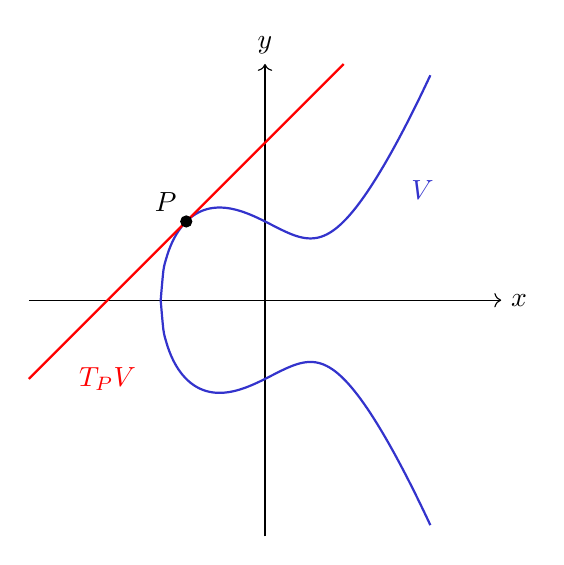
\begin{tikzpicture}
  % Draw axes
  \draw[->] (-3, 0) -- (3, 0) node[right] {$x$};
  \draw[->] (0, -3) -- (0, 3) node[above] {$y$};

  % Plot the curve y^2 = x^3 - x + 1 manually
  \draw[thick, blue, samples=100, smooth, domain=-1.32472:2.1, variable=\x] 
    plot ({\x}, {sqrt((\x)^3 - (\x) + 1)});
  \draw[thick, blue, samples=100, smooth, domain=-1.32472:2.1, variable=\x] 
    plot ({\x}, {-sqrt((\x)^3 - (\x) + 1)});

  % Tangent line y = (x + 1) + 1
  \draw[thick, red, domain=-3:1] plot(\x, {(\x+1)+1});

  % Mark the point (-1, 1)
  \filldraw[black] (-1, 1) circle (2pt) node[above left] {$P$};

  % Labels for the curve and tangent line
  \node[blue] at (2, 1.4) {$V$};
  \node[red] at (-2, -1) {$T_PV$};
\end{tikzpicture}
\caption{The tangent space of $V = \bV(Y^2 - X^3 + X - 1)$ and $P=(-1, 1)$, which is given by $T_PV = \bV(-2(X+1)+2(Y-1))$.}
\label{figure:tangentspace}
\end{figure}

Now let $V\subseteq\AA^n$ be any algebraic set.
Given $f\in\bI(V)$, we compute $f_P^{(1)}$ using Equation \ref{equationtangent}.
The \emph{tangent space} of $V$ at $P$ is
$$T_PV := \bigcap_{f\in\bI(V)} \bV(f_P^{(1)}).$$
In other words, $T_PV$ is the intersection of all affine subspaces tangent at $P$ to some $f$ in the ideal $\bI(V)$ defining $V$.

We now explain how the intersection defining $T_PV$ may be replaced with a finite intersection.
Suppose $f_1, \ldots, f_m$ generate $\bI(V)$.
Then for any $f = \sum_{j=1}^m h_j f_j \in \bI(V)$ and $P \in V$, one readily computes that
\begin{align*}
	f_P^{(1)} &= \sum_{j=1}^m h_j(P) \sum_{i=1}^n \frac{\partial f_j}{\partial X_i}(P)(X_i-a_i).
\end{align*}
Thus $f_P^{(1)}$ is a linear combination of the polynomials $f_{j,P}^{(1)}$.
It follows that $f_P^{(1)}$ vanishes whenever all the $f_{j,P}^{(1)}$ do, so
$$\bigcap_{j=1}^m \bV(f_{j,P}^{(1)}) \subseteq \bigcap_{f \in \bI(V)} \bV(f_P^{(1)}).$$
The opposite inclusion is clear, and therefore
$$T_PV=\bigcap_{j=1}^m \bV(f_{j,P}^{(1)}).$$

We now explain why $T_PV$ is a vector space over $k$ and therefore has a dimension.
It is clear that that zero vector is the point $P$.
The addition and scalar multiplication is defined as follows: if $Q_1, Q_2 \in \AA^n$ lying in $T_PV$ are written $Q_i = \tilde Q_i + P$, then
$$Q_1 + Q_2 := (\tilde Q_1 + \tilde Q_2) + P, \qquad\qquad \lambda \cdot Q_i := \lambda \tilde Q_i + P, \,\,\, \lambda \in k.$$
This is the usual vector space structure on $k^n = \AA^n$ if the origin is translated to $P$.

We now define the \emph{dimension} of an irreducible algebraic set $V$ by
$$\dim V := \min\{\dim T_PV : P \in V\}.$$
A point $P \in V$ is called \emph{non-singular} if $\dim T_PV = \dim V$ and \emph{singular} if $\dim T_P V > \dim V$.
We denote the set of non-singular and singular points by $V_{\text{non-sing}}$ and $V_{\text{sing}}$, respectively;
$V$ is called non-singular if it is non-singular at every point.

We now give examples computing tangent spaces and dimensions of algebraic sets.

\begin{example}
\begin{enumerate}
\item
Consider the trivial example $V = \AA^n$.
The ideal $\bI(V)$ is generated by $f = 0$, which for any $P$ has first-order part $f_P^{(1)} = 0$.
Then $T_PV = \bV(f_P^{(1)}) = \AA^n$, i.e., $T_PV$ is the vector space $k^n$ with the origin translated to $P$.
As expected, $\dim V = n$, and $\AA^n$ is non-singular.

\item
Consider $V = \bV(f) \subseteq \AA^2$, where $f = Y^2 - X^3 - 2X^2$.
For $P = (a, b)$, one computes
$$f_P^{(1)} = \frac{\partial f}{\partial X}(P)(X-a) + \frac{\partial f}{\partial Y}(P)(Y-b) = a(-3a-4)(X - a) + 2b(Y-b).$$ 
The tangent space $\bV(f_P^{(1)})$ is a line if at least one of the coefficients $a(-3a-4)$ and $2b$ is non-zero, and all of $\AA^2$ otherwise.
Of the points $(0, 0)$ and $(-\frac{4}{3}, 0)$ that make both coefficients vanish, only $(0, 0)$ lies in $V$.
Therefore, $T_PV$ is a line for all points in $V\setminus\{(0, 0)\}$, and $T_{(0,0)}V = \AA^2$.
Thus, $\dim V = 1$ and $P = (0, 0)$ is a singular point of $V$.
\end{enumerate}
\end{example}

\begin{figure}[H]
     \begin{subfigure}[b]{0.49\textwidth}
          \centering
          \resizebox{\linewidth}{!}{
		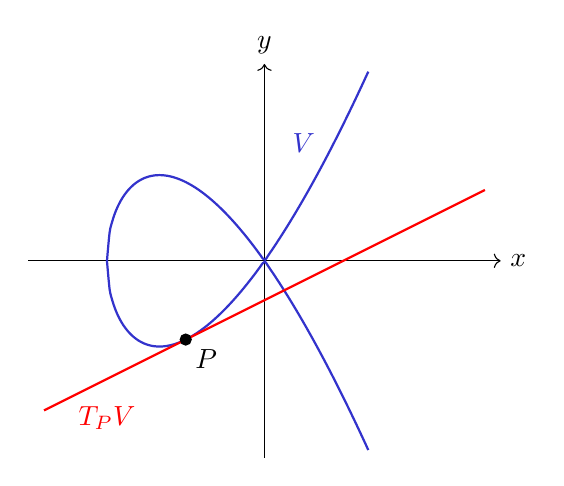
\begin{tikzpicture}
		  % Draw axes
		  \draw[->] (-3, 0) -- (3, 0) node[right] {$x$};
		  \draw[->] (0, -2.5) -- (0, 2.5) node[above] {$y$};
		
		  % Plot the curve y^2 = x^3 + 2x^2 manually
		  \draw[thick, blue, samples=100, smooth, domain=-2:1.32, variable=\x] 
		    plot ({\x}, {sqrt((\x)^3 + 2*(\x)^2)});
		  \draw[thick, blue, samples=100, smooth, domain=-2:1.32, variable=\x] 
		    plot ({\x}, {-sqrt((\x)^3 + 2*(\x)^2)});
		
		  % Tangent line y = 2 + (9/4)(X-1)
		  \draw[thick, red, domain=-2.8:2.8] plot(\x, {(1/2)*(\x+1)-1});
		
		  % Mark the point (-1, -1)
		  \filldraw[black] (-1, -1) circle (2pt) node[below right] {$P$};
		
		  % Labels for the curve and tangent line
		  \node[blue] at (0.5, 1.5) {$V$};
		  \node[red] at (-2, -2) {$T_PV$};
		\end{tikzpicture}
          }  
          \caption*{$P=(-1, -1)$}
          \label{fig:A}
     \end{subfigure}
     \begin{subfigure}[b]{0.49\textwidth}
          \centering
          \resizebox{\linewidth}{!}{
		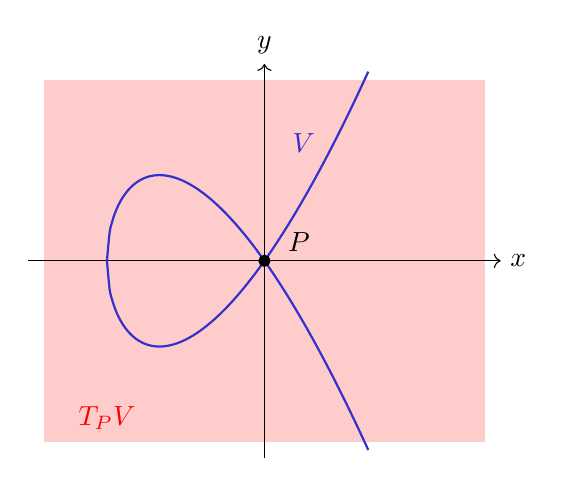
\begin{tikzpicture}
		  % Shading the background to represent T_PV being all of A^2
		  \fill[red!20] (-2.8, -2.3) rectangle (2.8, 2.3);
		
		  % Draw axes
		  \draw[->] (-3, 0) -- (3, 0) node[right] {$x$};
		  \draw[->] (0, -2.5) -- (0, 2.5) node[above] {$y$};
		
		  % Plot the curve y^2 = x^3 - x + 1 manually
		  \draw[thick, blue, samples=100, smooth, domain=-2:1.32, variable=\x] 
		    plot ({\x}, {sqrt((\x)^3 + 2*(\x)^2)});
		  \draw[thick, blue, samples=100, smooth, domain=-2:1.32, variable=\x] 
		    plot ({\x}, {-sqrt((\x)^3 + 2*(\x)^2)});
		
		  % Mark the point (0, 0)
		  \filldraw[black] (0, 0) circle (2pt) node[above right] {\,\,\,$P$};

		  % Labels for the curve and tangent line
		  \node[blue] at (0.5, 1.5) {$V$};
		  \node[red] at (-2, -2) {$T_PV$};
		\end{tikzpicture}
          }  
          \caption*{$P=(0,0)$}
          \label{fig:B}
     \end{subfigure}
     \caption{Two tangent spaces of $V = \bV(Y^2-X^3-2X^2)$.}
     \label{figure:}
\end{figure}

In the singular example above, $V_{\text{non-sing}}$ is the complement of a single point, in particular, it is an open subset of $V$.
This gives an example of the general fact that the set of non-singular points is an open subset of $V$ \cite[Proposition 6.3]{Reid88}.

Although the description we have given for $T_PV$ in terms of first-order parts of polynomials is geometrically intuitive, it depends on the embedding of $V$ into affine space.
We now prove a theorem which gives an intrinsic description of $T_PV$ in terms of ideals in the coordinate ring of $V$.

Suppose $V$ is an algebraic set in $\AA^n$ with $P \in V$.
Changing coordinates if necessary, we assume without loss of generality that $P=(0, \ldots, 0)$.
Now $T_PV$ is a vector subspace of $k^n$.
Write $\frakm_P\subseteq k[V]$ for the maximal ideal of regular functions vanishing at $P$, and denote by $M_P$ the ideal $(X_1, \ldots, X_n) \subseteq k[X_1,\ldots, X_n]$.
Note that we have $\frakm_P=M_P/\bI(V)$.
We are now ready to prove the theorem.

\begin{theorem}[{\cite[\S 6.8]{Reid88}}]
There is a natural isomorphism of vector spaces
$$(T_PV)^* \cong \frakm_P/\frakm_P^2,$$
where $(T_PV)^*$ is the algebraic dual vector space of $T_PV$.
\end{theorem}
\begin{proof}
We first prove the special case $V=\AA^n$, where we must show $M_P/M_P^2\cong(k^n)^*$.
Note that $\{X_1, \ldots, X_n\}$ is a basis for $(k^n)^*$.
As $P=(0, \ldots, 0)$, the first-order part
$$f_P^{(1)}=\sum_{i=1}^n \frac{\partial f}{\partial X_i}(P) X_i$$
is a linear form on $k^n$.
This gives rise to the map $d : M_P\to(k^n)^*$ defined by $f \mapsto f_P^{(1)}$.
It suffices to show $d$ is surjective with kernel $M_P^2$.
Note $d$ is surjective since the images of the $X_i$ form a basis for $(k^n)^*$.
Next, a general $f \in M_P$ can be written
$$f=\sum_{i=1}^n c_i X_i + \text{higher order terms},$$
for some $c_i \in k$.
Since $P=(0,\ldots,0)$, the first-order part equals
$$f_P^{(1)} = \sum_{i=1}^n c_i X_i.$$
Therefore $f \in \ker d$ if and only if each $c_i$ equals zero.
This is equivalent to $f$ lying in $M_P^2$, as $M_P^2$ is generated by the monomials $X_i X_j$.

For the general case, we show $(T_PV)^*$ and $\frakm_P/\frakm_P^2$ are both isomorphic to
$$M_P/(M_P^2+\bI(V)).$$

We now show $(T_PV)^* \cong M_P/(M_P^2+\bI(V))$.
Observe that we have the surjective restriction map $(k^n)^* \to (T_PV)^*$.
Composing $d$ with this restriction map yields another map
$$D:M_P \to (k^n)^* \to (T_PV)^*,$$
which is clearly surjective.
To prove the desired isomorphism, it suffices to show $\ker D = M_P^2+\bI(V)$.
We give equivalent conditions for $f$ to lie in $\ker D$.
By definition of $D$, the map $f$ lies in $\ker D$ if and only if $f_P^{(1)} \big|_{T_PV} = 0$.
If $g_j \in \bI(V)$ denote generators for $\bI(V)$, we know $T_PV = \bigcap_j \bV(g_{j,P}^{(1)}).$
Then $f_P^{(1)} \big|_{T_PV}=0$ if and only if 
$$f_P^{(1)} = \sum_j a_j g_{j,P}^{(1)}$$
for some $a_j \in k$.
The above equality is equivalent to $f$ and $\sum_j a_j g_j$ only differing by quadratic terms.
In other words, it is equivalent to the inclusion
$$f - \sum_j a_j g_j \in M_P^2,$$
which is the same as the inclusion $f \in M_P^2 + \bI(V)$.

To see $\frakm_P/\frakm_P^2 \cong M_P/(M_P^2+\bI(V))$, we find a surjective homomorphism $\varphi : M_P \to \frakm_P/\frakm_P^2$ with kernel $M_P^2+\bI(V)$. 
To this end, define $\varphi$ by $h \mapsto (h+\bI(V)) + \frakm_P^2$.
This is well-defined and surjective since $\frakm_P=M_P/\bI(V)$.
Also,
$$\ker \varphi = \{h \in M_P : h + \bI(V) \in \frakm_P^2\}=\{h \in M_P:h+\bI(V)\in M_P^2/\bI(V)\}=M_P^2+\bI(V).$$
\end{proof}

The above theorem motivates the following definition:

\begin{definition}
Let $V = \Spec(A)$ be an affine variety and $P$ a point in $V$ corresponding to the maximal ideal $\frakm$.
The Zariski tangent space of $V$ at $P$ is
$$T_PV := (\frakm / \frakm^2)^*.$$
\end{definition}

We will use this characterisation of $T_PV$ in Theorem \ref{theorem:singularities} to determine when a toric variety is non-singular.






\newpage
\section{Convex geometry}\label{chapter:convexgeometry}
An affine toric variety is an affine variety defined using a cone in a vector space.
Many properties of the variety are determined by properties of the cone.
Thus, to study toric varieties, it is important to understand the convex geometry of cones.
The goal of this chapter is to study the convex geometry we will need to study toric varieties.

We begin by defining convex cones and providing examples.
Analogous to how vector spaces have dual spaces, cones have dual cones.
One of the main results we prove in this chapter is that dualising a convex cone twice yields the same cone---this is a fundamental fact, but the proof is non-trivial.
Studying cones is more subtle than studying vector spaces because cones are not linear objects.
For example, a cone may have different dimension to its dual (cf.\ Example \ref{example:conesandduals}), unlike finite-dimensional vector spaces, where the dimension of the dual is the same.

In the context of toric varieties, the cones we are interested in have certain properties like being polyhedral, strongly convex, and rational.
An important part of this chapter is clearly defining these properties.
In Chapter \ref{chapter:affinetoricvarieties}, we will see how these properties have consequences for toric varieties.






\subsection{Convex cones}\label{section:convexcones}
In this section, we define convex cones and their duals.
We also prove that dualising a cone twice yields the original cone.

Throughout this chapter, $N_\RR$ denotes a real vector space of finite dimension $n$, with algebraic dual space $M_\RR = N_\RR^*$.
We have the dual pairing $\langle \cdot, \cdot \rangle : M_\RR \times N_\RR \to \RR$ given by $\langle u, v \rangle := u(v)$.

A subset $\sigma \subseteq N_\RR$ is a cone if it is closed under non-negative scalar multiplication, i.e., $\lambda x \in \sigma$ for all $x \in \sigma$ and all $\lambda \in \RR_{\ge 0}$.
A set $\sigma \subseteq N_\RR$ is convex if for any two points in $\sigma$, the line segment joining them is contained in $\sigma$,
i.e., $x, y \in \sigma$ implies $\lambda x + (1 - \lambda) y \in \sigma$ for all $\lambda \in [0, 1]$.
Since cones are closed under positive scalar multiplication, a cone is convex if and only if it is closed under addition.

The dimension of a cone $\sigma$ is
$$\dim(\sigma) := \dim(\RR \cdot \sigma),$$
where $\RR\cdot\sigma = \sigma + (-\sigma)$ is the smallest vector subspace of $N_\RR$ containing $\sigma$.
We say $\sigma$ is non-degenerate if $\dim(\sigma) = \dim N_\RR$.

\begin{example}\label{example:cones}
\begin{enumerate}
\item
The two rays
$$\sigma_1 = \{(x, x), \, (x, 2x) : x \in \RR_{\ge 0}\}$$
is a cone but not convex.
We can ``fill in'' $\sigma_1$ to get the convex cone
$$\sigma_2 = \{(x, y) \in \RR_{\ge 0}^2 : x \le y \le 2 x\}.$$
We have $\dim (\sigma_1) = \dim(\sigma_2)=2$.

\item
An example of a convex cone in $\RR^3$ is
$$\sigma_3 = \{(x, r) \in \RR^2 \times \RR : \|x\| \le r\}.$$
We have $\dim(\sigma_3)=3$.
\end{enumerate}
\noindent
See Figure \ref{figure:cones} for plots of these cones.
\end{example}

\begin{figure}[h]
     \begin{subfigure}[b]{0.325\textwidth}
          \centering
          \resizebox{0.8 \linewidth}{!}{
              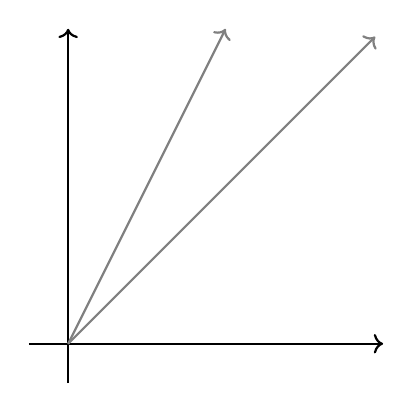
\begin{tikzpicture}
      		\draw[->,thick] (-0.5,0) -- (4,0);
      		\draw[->,thick] (0,-0.5) -- (0,4);
      		\draw[gray,thick,->,domain=0:3.9] plot (\x,\x);
      		\draw[gray,thick,->,domain=0:2] plot (\x,{2*\x});
    	    \end{tikzpicture}         
          }  
          \caption*{$\sigma_1$}
          \label{fig:A}
     \end{subfigure}
     \begin{subfigure}[b]{0.325\textwidth}
          \centering
          \resizebox{0.8 \linewidth}{!}{
              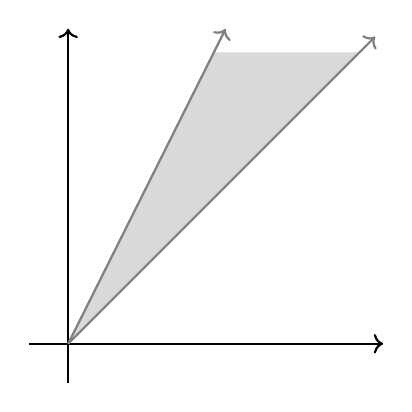
\begin{tikzpicture}
      		\draw[->,thick] (-0.5,0) -- (4,0);
      		\draw[->,thick] (0,-0.5) -- (0,4);
		    \fill[gray!30] (0,0) -- plot[domain=0:3.7] (\x,{\x}) -- plot[domain=1.85:0] (\x,{2*\x}) -- cycle;
      		\draw[gray,thick,->,domain=0:3.9] plot (\x,{\x});
      		\draw[gray,thick,->,domain=0:2] plot (\x,{2*\x});
    	\end{tikzpicture}          
          }  
          \caption*{$\sigma_2$}
          \label{fig:B}
     \end{subfigure}
     \begin{subfigure}[b]{0.325\textwidth}
          \centering
          \resizebox{\linewidth}{!}{
              \begin{tikzpicture}[tdplot_main_coords]
				\coordinate (O) at (0,0,1);
         		 \draw (0,0,-1) -- (O);
      			 \draw[->] (-5,0,1) -- (5,0,1) node[right] {};
     		 	 \draw[->] (0,-5,1) -- (0,5,1) node[right] {};
     		     \coneback[surface]{3}{2}{11}
     		     \draw[->] (O) -- (0,0,5) node[above] {};
      		     \conefront[surface]{3}{2}{13}
   	 \end{tikzpicture}
          }  
          \caption*{$\sigma_3$}
          \label{fig:C}
     \end{subfigure}
     \caption{The three cones in Example \ref{example:cones}.}
     \label{figure:cones}
\end{figure}

In linear algebra, dualising is an important operation which helps us to study a vector space.
In convex geometry, there is an similar notion for a cone, called the dual cone.
We will explore the relationship between a cone and its dual throughout this chapter.
We now give the definition:

\begin{definition}
Let $\sigma$ be a cone in $N_\RR$.
The dual cone $\sigma^\vee$ is
$$\sigma^\vee := \{u \in M_\RR : \langle u, v \rangle \ge 0 \text{ for all } v \in \sigma\}.$$
\end{definition}

We now give examples of cones and their duals.

\begin{example}\label{example:conesandduals}
Consider the vector space $N_\RR = \RR^n$.
Let $e_1, \ldots, e_n$ be the standard basis for $N_\RR$ and $e_1^*, \ldots, e_n^*$ the dual basis for $M_\RR$.
\begin{enumerate}
\item
Consider the cone $\sigma := \Span_{\RR_{\ge 0}}\{e_1, \ldots, e_n\}.$
Observe that a functional $\sum_{i=1}^n a_i e_i^*$ is in the dual cone if and only if $a_i \ge 0$ for all $i$.
Then $\sigma^\vee = \Span_{\RR_{\ge 0}}\{e_1^*, \ldots, e_n^*\}$.

\item
Now consider the cone $\sigma := \Span_{\RR_{\ge 0}}\{e_1^*, \ldots, e_r^*\}$, where $1 \le r \le n$.
The functional $\sum_{i=1}^n a_i e_i^*$ is in the dual cone if and only if $a_i \ge 0$ for all $1 \le i \le r$.
Thus, $\sigma^\vee = \Span_{\RR_{\ge 0}}\{e_1^*, \ldots, e_r^*, \pm e_{r+1}^*, \ldots, \pm e_n^*\}.$
Notice $\dim(\sigma)=r$ while $\dim(\sigma^\vee) = n$, showing $\sigma$ and $\sigma^\vee$ may have different dimensions.

\item
Let $n = 2$ and consider the cone $\sigma = \Span_{\RR_{\ge 0}} \{e_1, - e_1 + 2 e_2\}.$
To determine the elements $u\in\sigma^\vee$, we only need to check when $\langle u, v \rangle \ge 0$ for the generators $v = e_1$ and $v = -e_1 + 2 e_2$.
Then $u = a_1 e_1^* + a_2 e_2^* \in M_\RR$ lies in $\sigma^\vee$ precisely when the following two inequalities hold:
$$\langle u, e_1 \rangle = a_1 \ge 0, \quad \langle u, -e_1 + 2e_2 \rangle = -a_1 + 2a_2 \ge 0.$$
In view of Figure \ref{figureconeanddual}, we see  $\sigma^\vee = \Span_{\RR_{\ge 0}} \{2 e_1 + e_2, e_2\}.$
\end{enumerate}
\end{example}

\begin{figure}[H]
    \centering
    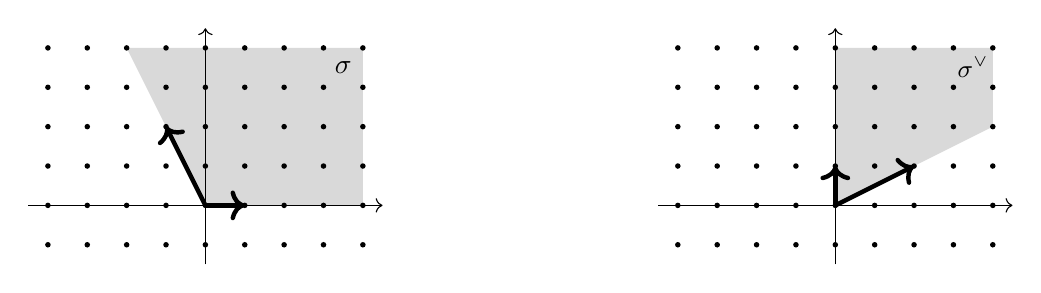
\begin{tikzpicture}
        % Left diagram
        \begin{scope}[shift={(-4,0)}]
            % Shaded area
            \fill[gray!30] (0,0) -- (-1,2) -- (2,2) -- (2,0) -- cycle;
            
            % Axes
            \draw[->] (-2.25,0) -- (2.25,0);
            \draw[->] (0,-0.75) -- (0,2.25);
            
            % Lattice points
            \foreach \x in {-2,-1.5,-1,-0.5,0,0.5,1,1.5,2}
                \foreach \y in {-0.5,0,0.5,1,1.5,2}
                    \fill (\x,\y) circle (1pt);

            % Vectors
            \draw[->, ultra thick] (0,0) -- (0.5,0);
            \draw[->, ultra thick] (0,0) -- (-0.5,1);
            \node at (1.75, 1.75) {$\sigma$};
        \end{scope}
        
        % Right diagram
        \begin{scope}[shift={(4,0)}]
            % Shaded area
            \fill[gray!30] (0,0) -- (0,2) -- (2,2) -- (2, 1) -- cycle;
            
            % Axes
            \draw[->] (-2.25,0) -- (2.25,0);
            \draw[->] (0,-0.75) -- (0,2.25);
            
            % Lattice points
            \foreach \x in {-2,-1.5,-1,-0.5,0,0.5,1,1.5,2}
                \foreach \y in {-0.5,0,0.5,1,1.5,2}
                    \fill (\x,\y) circle (1pt);

            % Vectors
            \draw[->, ultra thick] (0,0) -- (0,0.5);
            \draw[->, ultra thick] (0,0) -- (1,0.5);
            \node at (1.75, 1.75) {\small{$\sigma^\vee$}};
        \end{scope}
    \end{tikzpicture}
    \caption{The cone $\sigma=\Span_{\RR_{\ge 0}} \{e_1, - e_1 + 2 e_2\}$ and its dual.}
     \label{figureconeanddual}
\end{figure}

The following theorem relates a cone to its dual and has many important consequences.
For example, it is not obvious that dualising a cone twice yields the original cone, but the theorem establishes this fact (cf.\ Corollary \ref{corollary:doubledual}).
To state the theorem, we need to define a topology on $N_\RR$.
Choose any norm on $N_\RR$ and define the topology to be the one induced by that norm.
All norms on a finite-dimensional real vector space induce the same topology, so the topology is independent of the choice of norm.

\begin{theorem}[{\cite[\S 1.2]{Fulton93}}]\label{theorem:dualcone}
Let $\sigma$ be a topologically closed convex cone in $N_\RR$.
If $v \notin \sigma$, then there exists $u \in \sigma^\vee$ such that $\langle u, v \rangle <0.$
\end{theorem}

References such as \cite{Fulton93}, \cite{CLS11}, and \cite{Oda88} omit a proof of Theorem \ref{theorem:dualcone}, but we present one, following \cite{BV04}.
We begin with a lemma from analysis:

\begin{lemma}\label{lemma:mindistance}
Let $A$ and $B$ be disjoint, topologically closed subsets of a Euclidean vector space $(V, (\cdot,\cdot))$, and assume $A$ is compact.
Then there exist $a_{\text{min}} \in A$ and $b_{\text{min}} \in B$ which minimise the distance $\|a-b\|$ over all $a \in A$ and $b \in B$.
(Here $\|\cdot\|$ is the norm induced by $(\cdot,\cdot)$.)
\end{lemma}
%%%% THIS IS A WIKIPEDIA PROOF; FIND A REFERENCE %%%
\begin{proof}
Take arbitrary $x \in A$ and $y \in B$ and set $r_1 := \|x-y\| > 0$.
Since $A$ is compact, it is bounded by a closed ball of some radius $r_2 > 0$.
Let $S := B \cap \overline{B_{r_1+r_2}(x)},$ which is non-empty since $y \in S$.
Since the distance function is continuous and $A \times S$ is compact, there exists $(a_{\text{min}}, b_{\text{min}}) \in A \times S$ minimising the distance $\|a - b\|$ for all pairs of points in $A \times S$.
We claim that this is in fact the minimum for all pairs of points in $A \times B$.
Suppose to the contrary that there is $(\alpha,\beta) \in A \times B$ with $\|\alpha - \beta\| < \|a_{\text{min}} - b_{\text{min}}\|$. 
In particular, since $\|a_{\text{min}} - b_{\text{min}}\|\le r_1$, $\|\alpha - \beta\| < r_1$ and so
$\|x - \beta\| \le \|x- \alpha\| + \|\alpha - \beta\| < r_2 + r_1.$
This implies $\beta$ lies in $S$, contradicting that $\|a_{\text{min}} - b_{\text{min}}\|$ attained the minimum distance for pairs in $A \times S$.
\end{proof}

The proof of Theorem \ref{theorem:dualcone} follows from the following hyperplane separation theorem, which says that for certain sets, we can find a hyperplane so that each set lies in a different half-space.

\begin{theorem}[Hyperplane separation theorem {\cite[\S 2.5.1]{BV04}}]\label{hyperplaneseparation}
Under the assumptions of Lemma \ref{lemma:mindistance}, there exists $w \in V\setminus\{0\}$ and $\lambda \in \RR$ such that for all $a \in A$, $(w, a) \le \lambda$, and for all $b \in B$, $(w, b) \ge \lambda$.
\end{theorem}

\begin{proof}
Lemma \ref{lemma:mindistance} yields $a_{\text{min}} \in A$ and $b_{\text{min}} \in B$ minimising the distance between points in $A$ and points in $B$.
Then the desired $w$ and $\lambda$ are
$$w := b_{\text{min}} - a_{\text{min}}, \qquad\text{and}\qquad \lambda := \frac{1}{2}(b_{\text{min}} - a_{\text{min}}, b_{\text{min}} + a_{\text{min}}).$$
The hyperplane defined by $(w, \cdot) = \lambda$ is orthogonal to the line segment joining $a_{\text{min}}$ and $b_{\text{min}}$ and passes through the midpoint.
Let us prove that $(w, b) \ge \lambda$ for all $b \in B$ (a similar argument shows $(w, a) \le \lambda$ for all $a \in A$).
Proceeding by contradiction, assume that there exists $u \in B$ with $(w, u) < \lambda$.
Then by definition of $w$ and $\lambda$, this means 
$$0 > (w, u) -\frac{1}{2}(w, b_{\text{min}}+a_{\text{min}}) = (w, u-b_{\text{min}}+\frac{1}{2} (b_{\text{min}}-a_{\text{min}})) =(w, u-b_{\text{min}})+\frac{1}{2}\|w\|^2,$$
so in particular, $(w, u-b_{\text{min}})<0$.
Consider the function
$$g(t):=\|w+t(u-b_{\text{min}})\|^2.$$
Note that $g(0)=\|w\|$, and using the Leibniz rule for differentiating inner products, we see
$$g'(0) = 2 (w+t(u-b_{\text{min}}), u-b_{\text{min}}) \big|_{t=0} = 2 (w, u-b_{\text{min}}) < 0.$$
This implies that for small $t > 0$, $g(0) > g(t)$.
In other words,
$$\|b_{\text{min}} - a_{\text{min}}\| > \|b_{\text{min}} + t(u - b_{\text{min}}) - a_{\text{min}}\|.$$
But $B$ is convex and contains $b_{\text{min}}$ and $u$, so $B$ also contains $(b_{\text{min}} + t (u - b_{\text{min}}))$.
This contradicts the minimality of $\|b_{\text{min}} - a_{\text{min}}\|$.
\end{proof}

To prove Theorem \ref{theorem:dualcone}, we use the hyperplane separation theorem to find a certain hyperplane containing zero, which gives rise to the desired functional $u\in\sigma^\vee$.

\begin{proof}[Proof of Theorem \ref{theorem:dualcone} \textup{(\cite[Example 2.20]{BV04})}]
Fix a basis $e_1, \ldots, e_n$ for $N_\RR$ and endow $N_\RR$ with the inner product which makes the basis orthonormal.
Since $\sigma$ is topologically closed and $v \notin \sigma$, there exists $\varepsilon > 0$ such that $\overline{B_\varepsilon(v)}$ does not intersect $\sigma$.
By Theorem \ref{hyperplaneseparation}, there exist $w \in N_\RR$ and $\lambda \in \RR$ such that $(w, x) \ge \lambda$ for all $x \in \sigma$ and $(w, y) \le \lambda$ for all $y \in \overline{B_\varepsilon(v)}$.
In fact, we must have $\lambda \le 0$ since $0$ lies in $\sigma$.

We claim that $(w, x) \ge 0$ for all $x \in \sigma$ and $(w, v) < 0$.
This completes the proof, as then $u$ defined by $x \mapsto (w, x)$ is a linear form in $\sigma^\vee$ with $\langle u, v \rangle < 0$.
To see the first claim, suppose there exists $x \in \sigma$ with $(w, x) =: \lambda' < 0$.
Then for any $s \in \RR_{\ge 0}$, $s x \in \sigma $ and $(w, s x) = s \lambda'$, contradicting that $\{(w, x) : x \in \sigma\}$ is bounded from below.
To see the second claim, we just need to show $(w, v) \ne 0$.
Suppose we had $(w, v) = 0$.
As $y := v + \frac{\varepsilon w}{\|w\|}$ lies in $\overline{B_\varepsilon(v)}$, we get
$$\lambda \ge (w, y) = (w, v + \varepsilon w/\|w\|) = \varepsilon \|w\| > 0,$$
contradicting that $\lambda \le 0$.
\end{proof}

\begin{corollary}\label{corollary:doubledual}
Let $\sigma$ be a topologically closed cone in $N_\RR$.
Then $(\sigma^\vee)^\vee = \sigma$.
\end{corollary}
\begin{proof}
If $v \in \sigma$, then $\langle u, v\rangle \ge 0$ for all $u \in \sigma^\vee$, so $v \in (\sigma^\vee)^\vee$.
If $v \notin \sigma$, then Theorem \ref{theorem:dualcone} implies there exists $u \in \sigma^\vee$ with $\langle u, v \rangle < 0$ so that $v \notin (\sigma^\vee)^\vee$.
\end{proof}





\subsection{Polyhedral cones}\label{polyhedralcones}
In this section, we define a class of convex cones called polyhedral cones---these are cones with a finite set of generators.
The cones associated to toric varieties are always polyhedral.
We also define and study faces of polyhedral cones, which are important subsets of the cone.

\begin{definition}\label{definition:convexpolyhedral}
A subset $\sigma$ of $N_\RR$ is called a (convex) polyhedral cone if
$$\sigma = \Span_{\RR_{\ge 0}} \{v_1, \ldots, v_r\}$$
for a finite set of generators $v_1, \ldots, v_r \in N_\RR$.
\end{definition}

It follows from the definition that convex polyhedral cones are indeed convex cones in the sense defined in \S \ref{section:convexcones}.
Every example of convex cones we have seen so far has been polyhedral, except for $\sigma_3 = \{(x, r) \in \RR^2 \times \RR : \|x\| \le r\}$ in Example \ref{example:cones}.

One definition of a convex polyhedron is a finite intersection of closed half-spaces in $\RR^3$.
The name polyhedral is justified by the following result:

\begin{theorem}
A cone satisfies Definition \ref{definition:convexpolyhedral} if and only if it is a finite intersection of closed half-spaces.
\end{theorem}
\begin{proof}
Later, in Proposition \ref{proposition:dualdescription}, we give a dual description of polyhedral cones, showing they are finite intersections of closed half-spaces.
The converse is proven in \cite[1.3.13]{DLHK13}.
\end{proof}

We now define the faces of a polyhedral cone.
Any $u \in M_\RR$ defines a subspace of $N_\RR$ in the following manner:
$$u^\perp = \{v \in N_\RR : \langle u, v \rangle = 0\}.$$
When $u$ is non-zero, $\dim u^\perp = n -1$.
The notation suggests we can intuitively think of $u^\perp$ as the orthogonal complement of $u$, though this interpretation is not strictly accurate since $\langle \cdot, \cdot \rangle$ is not an inner product.
A face $\tau$ of $\sigma$ is a set of the form 
$$\tau = \sigma \cap u^\perp,$$
for some $u \in \sigma^\vee$.
In other words, a face is the intersection of $\sigma$ with a hyperplane, such that $\sigma$ lies in the positive half-space of the hyperplane.
When $u = 0$, we have $\sigma \cap u^\perp = \sigma$, so $\sigma$ is a face of itself.
A face of codimension 1 is called a facet.
Let us give a basic example to illustrate these definitions.

\begin{example}
Consider $\sigma = \Span_{\RR_{\ge 0}} \{e_1, e_2\}$ in $N_\RR = \RR^2$.
We saw in Example \ref{example:conesandduals} that $\sigma^\vee = \Span_{\RR_{\ge 0}}\{e_1^*, e_2^*\}$.
Suppose $u = b_1 e_1^* + b_2 e_2^*$ lies in $\sigma^\vee$.
If $b_1$ and $b_2$ are both non-zero, then
$$\sigma \cap u^\perp = \{(a_1, a_2) \in \RR_{\ge 0}^2 : a_1 b_1 + a_2 b_2 = 0\} = \{0\}.$$
If $b_1 \ne 0$ but $b_2 = 0$, then
$$\sigma \cap u^\perp = \{(a_1, a_2) \in \RR_{\ge 0}^2 : a_1 b_1 = 0\} = \Span_{\RR_{\ge 0}}\{e_2\}.$$
Similarly, if $b_1 = 0$ but $b_2 \ne 0$, then $\sigma \cap u^\perp = \Span_{\RR_{\ge 0}} \{e_1\}.$
Figure \ref{figure:facesandnormals} shows the faces of $\sigma$ and functionals which define the faces.
\end{example}

\begin{figure}[H]
    \centering
    % Left subfigure
    \begin{subfigure}[b]{0.45\textwidth}
        \centering
        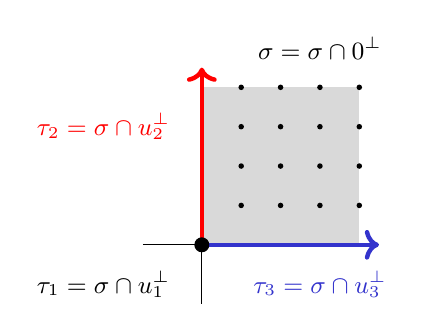
\begin{tikzpicture}
            % Shaded area
            \fill[gray!30] (0,0) -- (0,2) -- (2,2) -- (2,0) -- cycle;
            
            % Axes
            \draw[-] (-.75,0) -- (2.25,0);
            \draw[-] (0,-0.75) -- (0,2.25);
            
            % Lattice points
            \foreach \x in {0.5,1,1.5,2}
                \foreach \y in {0.5,1,1.5,2}
                    \fill (\x,\y) circle (1pt);

            % Vectors
            \draw[->, ultra thick, red] (0,0) -- (0,2.25);
            \draw[->, ultra thick, blue] (0,0) -- (2.25,0);
            \filldraw[black] (0, 0) circle (2.5pt);

            % Labels
            \node at (1.5, 2.5) {\small{$\sigma = \sigma \cap 0^\perp$}};
            \node[red] at (-1.25, 1.5) {\small{$\tau_2 = \sigma \cap u_2^\perp$}};
            \node[blue] at (1.5, -0.5) {\small{$\tau_3 = \sigma \cap u_3^\perp$}};
            \node at (-1.25, -0.5) {\small{$\tau_1 = \sigma \cap u_1^\perp$}};
        \end{tikzpicture}
        %\caption{Left diagram}
        %\label{fig:left_diagram}
    \end{subfigure}
    \hspace{-0.05\textwidth} % Creates equal spacing between the subfigures
    % Right subfigure
    \begin{subfigure}[b]{0.45\textwidth}
        \centering
        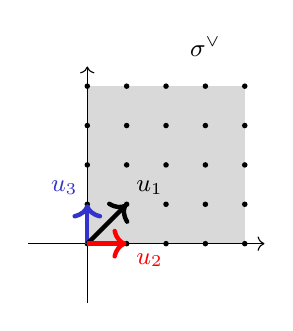
\begin{tikzpicture}
            % Shaded area
            \fill[gray!30] (0,0) -- (0,2) -- (2,2) -- (2, 0) -- cycle;
            
            % Axes
            \draw[->] (-.75,0) -- (2.25,0);
            \draw[->] (0,-0.75) -- (0,2.25);
            
            % Lattice points
            \foreach \x in {0,0.5,1,1.5,2}
                \foreach \y in {0,0.5,1,1.5,2}
                    \fill (\x,\y) circle (1pt);

            % Vectors
            \draw[->, ultra thick, blue] (0,0) -- (0,0.5);
            \draw[->, ultra thick] (0,0) -- (0.5,0.5);
            \draw[->, ultra thick, red] (0,0) -- (0.5,0);
            \node at (1.5, 2.5) {\small{$\sigma^\vee$}};

            % Labels
            \node[red, below right] at (0.5,0) {\small{$u_2$}};
            \node[blue, above left] at (0, 0.5) {\small{$u_3$}};
            \node[above right] at (0.5, 0.5) {\small{$u_1$}};
        \end{tikzpicture}
        %\caption{Right diagram}
        %\label{fig:right_diagram}
    \end{subfigure}
    \caption{The faces of $\sigma = \Span_{\RR_{\ge 0}}\{e_1, e_2\}$ and functionals defining them.}
    \label{figure:facesandnormals}
\end{figure}

We collect some basic properties of faces in the following proposition.

\begin{proposition}
Let $\sigma$ be a convex polyhedral cone.
\begin{enumerate}
\item A face of $\sigma$ is also a convex polyhedral cone.
\item There are only finitely many faces of $\sigma$.
\item Any intersection of faces is a face.
\item If $\tau$ is a face of $\sigma$, then a face of $\tau$ is also a face of $\sigma$.
\item Any proper face is contained in a facet.
Any proper face is the intersection of all the facets containing it, and a face with codimension two is the intersection of exactly two facets.
\end{enumerate}
\end{proposition}
\begin{proof}
See \cite[\S 1.2]{Fulton93} or \cite[\S 1]{Zaman13}.
\end{proof}





\subsection{Dual description of cones}\label{section:dualdescription}
We have seen some basic objects of convex geometry---cones and their duals---as well as some properties cones may have, like being polyhedral.
It is natural to ask whether the dual of a polyhedral cone is also polyhedral.
It turns out that this is the case, and this is the main result of this section:

\begin{theorem}[{Farkas's Lemma \cite[\S 1.2]{Fulton93}}]\label{theorem:farkas}
The dual of a convex polyhedral cone is a convex polyhedral cone.
\end{theorem}

The proof relies on giving a dual description of a polyhedral cone as an intersection of closed half-spaces.
To prepare for this, we discuss some basic topology of polyhedral cones.

Recall the interior of a subset $S$ of a topological space is the set of points admitting an open neighbourhood contained in $S$.
The boundary of $S$ is the set of points in the closure of $S$ which do not lie in the interior.
The following proposition characterises the boundary of a non-degenerate polyhedral cone:

\begin{proposition}\label{proposition:boundary}
The boundary of a non-degenerate polyhedral cone is the union of its proper faces.
\end{proposition}
\begin{proof}
See \cite[\S 1.2]{Fulton93} or \cite[\S 1]{Zaman13}.
\end{proof}

We are ready to describe a polyhedral cone as an intersection of closed half-spaces.
We will need the following observation:
if $\sigma$ is non-degenerate and $\tau$ is a facet, then the functional $u_\tau \in \sigma^\vee$ such that $\tau = \sigma \cap u_\tau^\perp$ is unique up to positive scalar multiplication.
Indeed, any two such $u_\tau$ both vanish on the $(n-1)$-dimensional subspace $\RR \cdot \tau$, and their values on a point outside this subspace determine them, but these only differ by a positive scalar.
We now prove the result:

\begin{proposition}[{\cite[\S 1.2]{Fulton93}}]\label{proposition:dualdescription}
Let $\sigma$ be a non-degenerate cone in $N_\RR$ such that $\sigma \ne N_\RR$.
Then, $\sigma$ equals the intersection of half-spaces
$$H_\tau = \{v \in N_\RR : \langle u_\tau, v\rangle \ge 0\},$$
as $\tau$ ranges over the facets of $\sigma$.
\end{proposition}
\begin{proof}
The half-space $H_\tau$ does not depend on the choice of $u_\tau \in \sigma^\vee$ such that $\tau = \sigma \cap u_\tau^\perp$, since the functional $u_\tau$ is unique up to positive scalar multiplication.

If $v$ lies in $\sigma$, then $\langle u_\tau, v \rangle \ge 0$ for any facet $\tau$, since $u_\tau \in \sigma^\vee$.
Then $v$ lies in the intersection of half-spaces.

Conversely, suppose for the sake of contradiction that $v'$ is in the intersection of half-spaces but not in $\sigma$.
Since $\sigma$ is non-degenerate, Proposition \ref{proposition:boundary} implies there exists $v$ in the interior of $\sigma$.
There is a point $w$ on the line segment joining $v$ and $v'$ which also lies on the boundary of $\sigma$.
By Proposition \ref{proposition:boundary}, $w$ lies on a facet, say $\tau$.
Since $\langle u_\tau, v \rangle > 0$ and $\langle u_\tau, w \rangle = 0$, we have $\langle u_\tau, v' \rangle < 0$.
This contradicts that $v'$ lies in the intersection of the half-spaces.
\end{proof}

Proposition \ref{proposition:dualdescription} allows us to prove that the dual of a polyhedral cone is a polyhedral cone:

\begin{proof}[Proof of Theorem \ref{theorem:farkas}]
Suppose first that $\sigma$ is non-degenerate.
We show the $u_\tau$, where $\tau$ runs over the facets of $\sigma$, generate $\sigma^\vee$.
Suppose for the sake of contradiction there is $u \in \sigma^\vee$ which does not lie in the cone generated by the $u_\tau$.
Applying Theorem \ref{theorem:dualcone} to the cone generated by the $u_\tau$ tells us there exists $v \in N_\RR$ such that $\langle u_\tau, v\rangle \ge 0$ for all $\tau$, but $\langle u, v \rangle < 0$.
By Proposition \ref{proposition:dualdescription}, $v$ lies in $\sigma$, so $\langle u, v \rangle < 0$ contradicts that $u$ lies in $\sigma^\vee$.

Now suppose $\sigma$ spans $V$, a subspace strictly smaller than $N_\RR$.
Let $\tilde \sigma$ denote the cone $\sigma$ thought of as a cone in $V = \RR \cdot \sigma$.
Then $\tilde \sigma$ is non-degenerate so that $\tilde \sigma^\vee$ is a convex polyhedral cone in $V^* = N_\RR / V^\perp$.
Then $\sigma^\vee$ will be generated by lifts of generators of $\tilde \sigma^\vee$, along with vectors $u$ and $-u$, as $u$ ranges over a basis for $V^\perp$.
\end{proof}

Given generators for a polyhedral cone $\sigma$, it would be nice to find generators for the dual cone.
The proof we just saw tells us it is sufficient to find the functional $u_\tau$ for each facet $\tau$.

We describe an algorithm for finding the functionals $u_\tau$ when $\sigma$ is non-degenerate.
For each set of $n-1$ $\RR$-independent vectors in the generating set of $\sigma$, solve for $u \in M_\RR$ vanishing on them.
If $u$ changes sign on the rest of the generators, it does not lie in $\sigma^\vee$ and may be discarded.
Now suppose that one of $u$ and $-u$ is non-negative on the rest of the generators; without loss of generality we assume $u$ is.
In this case, $u$ lies in $\sigma^\vee$, the $n-1$ vectors generate a face $\tau$, and $u = u_\tau$ is the equation of the face.

Let us consider an example of applying this algorithm.

\begin{example}\label{example:3dconeanddual}
Let $N = \ZZ^3$ and $N_\RR = \RR^3$.
Consider $\sigma := \Span_{\RR_{\ge 0}}\{ e_1, e_2, e_1+e_3, e_2 + e_3\}$.
Observe that $e_1^*$ vanishes on $e_2$ and $e_2+e_3$, and is non-negative on all generators of $\sigma$.
Similarly, $e_1^*+e_2^*-e_3^*$ vanishes on $e_1+e_3$ and $e_2+e_3$ and is non-negative on $\sigma$.
Continuing the algorithm for finding the functionals $u_\tau$ which define facets, we see they are
$$u_{\tau_1} = e_1^*, \qquad u_{\tau_2} = e_2^*, \qquad u_{\tau_3} = e_3^*, \qquad u_{\tau_4} = e_1^* + e_2^* - e_3^*.$$
The dual cone is generated by $u_{\tau_1}, \ldots, u_{\tau_4}$, so
$$\sigma^\vee = \Span_{\RR_{\ge 0}} \{e_1^*, e_2^*, e_3^*, e_1^* +e_2^* - e_3^*\}.$$
\begin{figure}[h]
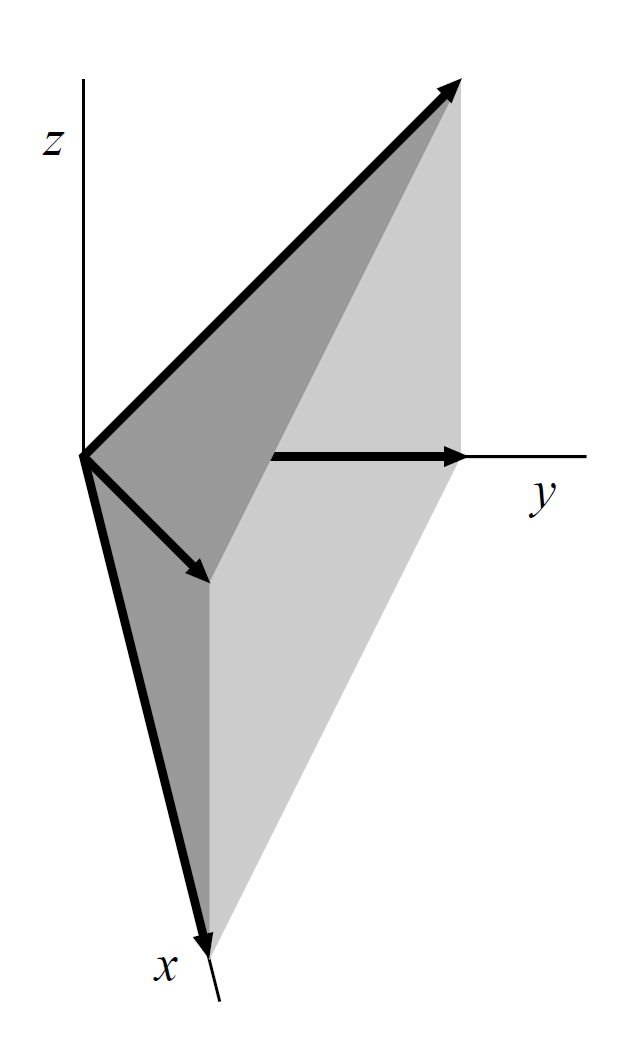
\includegraphics[width=0.2 \textwidth]{../images/cox cone example 2}
\caption{The cone $\sigma= \Span_{\RR_{\ge 0}}\{ e_1, e_2, e_1+e_3, e_2 + e_3\}$ \cite[Figure 2]{CLS11}.}
\label{figure:3dcone}
\end{figure}
\end{example}



\subsection{Strongly convex cones}
In this section, we define a class of polyhedral cones called strongly convex cones.
The cones used to study toric varieties are strongly convex.
We prove a useful proposition giving equivalent conditions for a cone to be strongly convex.
This involves a lemma providing a bijection between the faces of a cone and the faces of its dual.

We say a convex polyhedral cone is strongly convex if the origin of $N_\RR$ is a face.
Most of the cones we have seen in this chapter have been strongly convex.
An example of a polyhedral cone which is not strongly convex is the upper half-plane $\sigma = \Span_{\RR_{\ge 0}}\{e_1, -e_1, e_2\}$ in $N_\RR=\RR^2$.
The dual cone $\sigma^\vee$ is generated by $e_2^*$ and the only proper face is the $x$-axis.
Figure \ref{figure:strongconvexity} contains diagrams of two more cones: one which is strongly convex, and one which is not.

\begin{figure}[h]
\centering
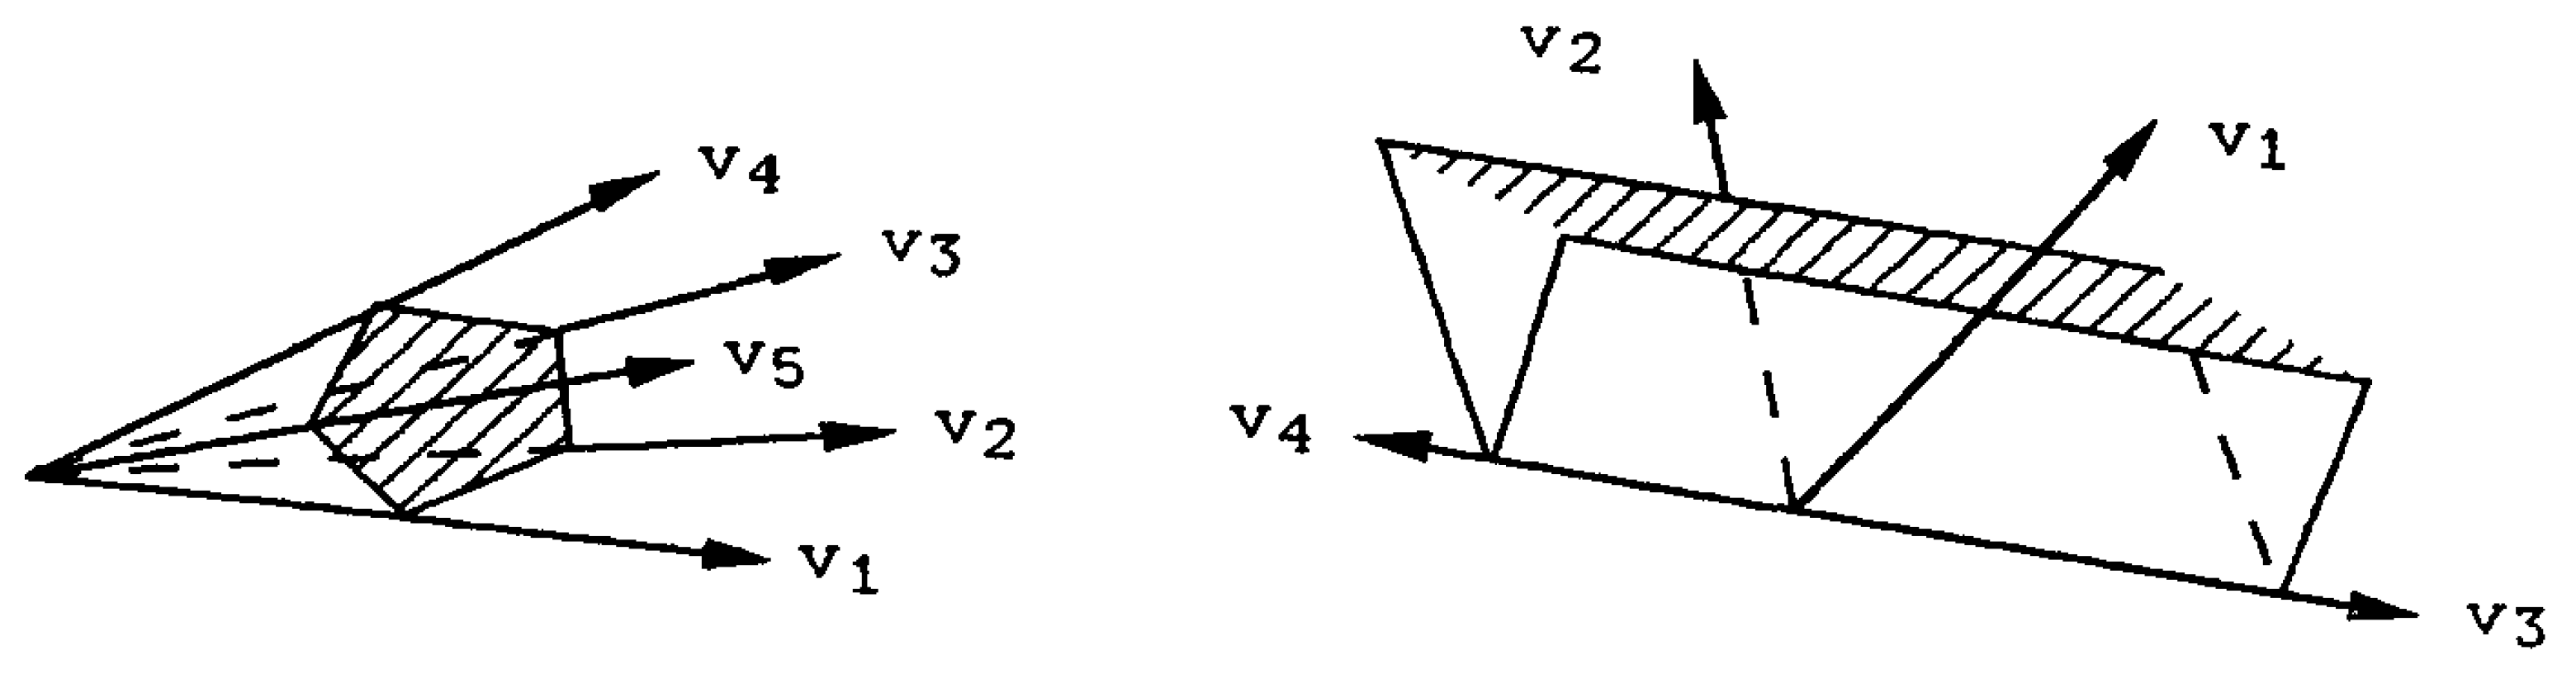
\includegraphics[width=0.8\textwidth]{../images/fultons_cones}
\caption{A strongly convex cone (left) and a non-strongly convex cone (right) \cite{Fulton93}.}
\label{figure:strongconvexity}
\end{figure}

Our goal is to give equivalent conditions for a cone to be strongly convex---the next lemma will help us do that.

For each face $\tau$ of $\sigma$, we define
$$\tau^\perp = \{u \in M_\RR : \langle u, v \rangle = 0 \text{ for all } v \in \tau\}.$$

\begin{lemma}\label{lemma:dualfaces}
If $\tau$ is a face of $\sigma$, then $\sigma^\vee \cap \tau^\perp$ is a face of $\sigma^\vee$, and
$$\dim(\tau) + \dim(\sigma^\vee \cap \tau^\perp) = \dim N_\RR.$$
Moreover, the map $\tau \mapsto \sigma^\vee \cap \tau^\perp$ is an inclusion-reversing bijection between the faces of $\sigma$ and the faces of $\sigma^\vee$.
In particular, the smallest face of $\sigma$ is $\sigma \cap (-\sigma) = (\sigma^\vee)^\vee \cap (\sigma^\vee)^\perp$.
\end{lemma}
\begin{proof}
See \cite[\S 1.2]{Fulton93} or \cite[\S 1]{Zaman13}.
\end{proof}

We can now give equivalent conditions for a cone to be strongly convex.

\begin{proposition}[{\cite[\S 1.2, Proposition 3]{Fulton93}}]\label{stronglyconvexprop}
For a convex polyhedral cone $\sigma$, the following conditions are equivalent:
\begin{enumerate}
\item $\sigma$ is strongly convex.
\item $\sigma \cap (-\sigma) = \{0\}$.
\item $\sigma$ contains no non-zero vector subspace of $N_\RR$.
\item $\sigma^\vee$ spans $M_\RR$.
\end{enumerate}
\end{proposition}
\begin{proof}
The largest vector subspace of $\sigma$ is $\sigma \cap (-\sigma)$, and this observation proves (2) and (3) are equivalent.
Lemma \ref{lemma:dualfaces} tells us $\sigma \cap(-\sigma)$ is also the smallest face of $\sigma$, so (1) and (2) are equivalent.
The dimension formula in Lemma \ref{lemma:dualfaces} applied to $\tau = \sigma \cap (-\sigma)$ says $\dim(\sigma \cap (-\sigma)) + \dim(\sigma^\vee) = \dim N_\RR$.
This gives the equivalence of (2) and (4).
\end{proof}





\subsection{Rational cones}\label{section:rationalcones}
To conclude this chapter, we introduce rational cones.
The cones used to study toric varieties are always rational (in addition to strongly convex).
Defining rational cones requires us to consider lattices in the vector spaces $N_\RR$ and $M_\RR$.

Recall $N_\RR$ and $M_\RR$ are dual vector spaces with dual pairing $\langle \cdot , \cdot \rangle : M_\RR \times N_\RR \to \RR$.
Now, let $N$ be a lattice in $N_\RR$.
This means $N$ is a free abelian subgroup of $N_\RR$ with rank $n = \dim N_\RR$ such that $\Span_\RR N = N_\RR$.
Concretely, $N$ is a lattice in $N_\RR$ if and only if there exists an $\RR$-basis for $N_\RR$ which is also a $\ZZ$-basis for $N$ \cite[\S 2.2]{Serre73}.
The relationship between $N$ and $N_\RR$ generalises the relationship between $\ZZ^n$ and $\RR^n$, and most of our examples will have $N = \ZZ^n$ and $N_\RR = \RR^n$ for simplicity.
We also let $M$ denote the dual lattice $\mathrm{Hom}_{\ZZ\text{-linear}}(N, \ZZ)$, which are the elements of $M_\RR = N_\RR^*$ taking integer values on $N$.

We say a polyhedral cone $\sigma$ is rational if its generators can be chosen from the lattice $N$.
All the examples of polyhedral cones we have seen are rational if our lattice is chosen to be $\ZZ^n$.
For example, when $N_\RR$ is $\RR^n$ and $N$ is $\ZZ^n$, the cone
$$\sigma = \Span_{\RR_{\ge 0}}\{e_1, \ldots, e_n\}$$
is rational, since the standard basis vectors $e_1, \ldots, e_n$ lie in $\ZZ^n$.
Similarly, when we choose $N_\RR$ to be $\RR^2$ and $N$ to be $\ZZ^2$, the cone
$$\sigma = \Span_{\RR_{\ge 0}}\{e_1, -e_1 + 2e_2\}$$
is rational.

Here are two facts about rational cones which we will need when studying affine toric varieties:
\begin{enumerate}
\item If $\sigma$ is a rational cone, then its faces are too \cite[Proposition 2]{Fulton93}.
\item If $\sigma$ is a rational cone, then the dual $\sigma^\vee$ is rational (meaning generators of $\sigma^\vee$ can be chosen from the dual lattice $M$).
This fact can be proven using the algorithm we presented in \S \ref{section:dualdescription} to find generators of $\sigma^\vee$.
In particular, when the generators of $\sigma$ lie in $N$, the algorithm can be used to find generators for $\sigma^\vee$ in $M$. 
\end{enumerate}

\newpage
\hfill










\newpage
\section{Affine toric varieties}\label{chapter:affinetoricvarieties}
Affine toric varieties are a class of algebraic varieties which are determined by a cone in a vector space.
There is a rich interplay between the algebraic geometry of the variety and the convex geometry of the cone.
Moreover, computations with the cone can often be done explicitly, which means toric varieties are useful to study as examples.

A toric variety $V$ is a normal\footnote{An affine variety is normal if its coordinate ring is integrally closed \cite[p.\ 29]{Fulton93}.} variety containing an algebraic torus $T$ as a dense open subset, such that $T$ acts on $V$ by an action which extends the natural action of $T$ on itself \cite[\S 1.1]{Fulton93}.
This definition is straightforward to state, but makes no reference to a cone in a vector space, so the relationship with convex geometry is unclear.

In this chapter, we use the convex geometry from the previous chapter to define affine toric varieties using cones.
Afterwards, we establish some fundamental properties, such as the existence of a dense torus which acts on the variety, and computing singularities.

Throughout this chapter, $N$ is a lattice in the vector space $N_\RR$ and $M$ is the dual lattice in $M_\RR = N_\RR^*$.
A cone $\sigma$ is always assumed to be polyhedral, strongly convex and rational.





\subsection{Semigroups and semigroup algebras}
In this section, we associate two algebraic objects with a cone: a semigroup and its semigroup algebra.
We also explain when these objects are finitely generated.
We will use semigroup algebras to define affine toric varieties in \S \ref{section:affinetoricvarieties}.

Recall a semigroup is a set with an associative binary operation.
All the semigroups we consider are commutative, so we will write the operation additively.
If $S$ is a semigroup and $T$ is a finite subset of $S$, we say $T$ generates $S$ if every element in $S$ can be written as a sum of elements of $T$.
A map between semigroups with identity $\varphi : S \to T$ is a homomorphism if it preserves the identity and $\varphi(x + y) = \varphi(x) + \varphi(y)$ for all $x$ and $y$ in $S$.

Let $\sigma$ be cone in $N_\RR$.
The semigroup of $\sigma$ is defined as
$$S_\sigma := \sigma^\vee \cap M.$$
In other words, $S_\sigma$ is the set of lattice points in the dual cone of $\sigma$.
Since $S_\sigma$ is a subsemigroup of the lattice $M$, it is abelian.
Also, $S_\sigma$ contains $0$, meaning it is a semigroup with identity.\footnote{In the literature, it is conventional to call $S_\sigma$ a semigroup, even though it is in fact a monoid.}
The following result tells us when $S_\sigma$ is finitely generated:

\begin{theorem}[Gordan's lemma {\cite[\S 1.2]{Fulton93}}]\label{gordanslemma}
If $\sigma$ is a rational convex polyhedral cone, then $S_\sigma$ is a finitely generated semigroup.
\end{theorem}
\begin{proof}
We know $\sigma^\vee$ is polyhedral and rational because $\sigma$ is (cf.\ Theorem \ref{theorem:farkas} and \S \ref{section:rationalcones}).
Then let $u_1, \ldots, u_s \in \sigma^\vee \cap M$ generate $\sigma^\vee$ as a cone.
Define
$$K = \left\{\sum_{i=1}^s t_i u_i : 0 \le t_i \le 1\right\} \subseteq M_\RR.$$
Since $K$ is compact and $M$ is discrete, the intersection $K \cap M$ is finite.
We claim $K \cap M$ generates $S_\sigma$.
%Note that $u_1, \ldots, u_s \in K \cap M$.
Suppose that $u \in S_\sigma$.
Then $u =\sum_{i=1}^s r_i u_i$ for some $r_i \in \RR_{\ge 0}$ since $u_1, \ldots, u_s$ generate $\sigma^\vee$.
Write each $r_i$ as $m_i + t_i$ for $m_i \in \ZZ_{\ge 0}$ and $0 \le t_i < 1$, so $u = \sum_{i=1}^s m_i u_i + \sum_{i=1}^s t_i u_i$.
Clearly $\sum_{i=1}^s t_i u_i$ lies in $K$.
Also, $\sum_{i=1}^s t_i u_i = u - \sum_{i=1}^s m_i u_i$ lies in $M$ since $u$ and $\sum_{i=1}^s m_i u_i$ lie in $M$ and $M$ is a group.
Then $\sum_{i=1}^s t_i u_i$ lies in $K \cap M$, and since $u_1, \ldots, u_s \in K \cap M$, we have $u = \sum_{i=1}^s m_i u_i + \sum_{i=1}^s t_i u_i \in \Span_{\ZZ_{\ge 0}} K \cap M$.
\end{proof}

Using the semigroup $S_\sigma = \sigma^\vee \cap M$, we can also construct the semigroup algebra $k[S_\sigma]$.
This construction is analogous to the construction of the group algebra using a group.
We now explain the details.

Given $S_\sigma$, the semigroup algebra $k[S_\sigma]$ is the algebra with basis of formal symbols
$$\{\chi^u : u \in S_\sigma\}.$$
The multiplication in $k[S_\sigma]$ is determined by addition in $S_\sigma$, in the following way:
$$\chi^u \chi^{u'} := \chi^{u + u'}.$$
The algebra $k[S_\sigma]$ is commutative and unital since $S_\sigma$ is.
Also, when $\sigma$ is rational, Gordan's lemma implies $S_\sigma$ and hence $k[S_\sigma]$ are finitely generated.
Specifically, if $u_1, \ldots, u_s$ generate $S_\sigma$, then $\chi^{u_1}, \ldots, \chi^{u_s}$ generate $k[S_\sigma]$.

As an example, let us consider the semigroup algebra corresponding to the trivial cone $\sigma = \{0\}$.
The dual cone $\sigma^\vee$ is all of $M_\RR$, so $S_\sigma = M_\RR \cap M = M$ and $k[S_\sigma]=k[M]$. 
Given a basis $\{e_1^*, \ldots, e_n^*\}$ for $M$, denote
$$X_i := \chi^{e_i^*} \in k[M].$$
As a semigroup, $M$ is generated by $\pm e_1^*, \ldots, \pm e_n^*$, so
$$k[M] = k[X_1, X_1^{-1}, \ldots, X_n, X_n^{-1}],$$
and $k[M]$ is the ring of Laurent polynomials in $X_1, \ldots, X_n$.
For any cone $\sigma$, the semigroup $S_\sigma$ is contained in $M$, so that $k[S_\sigma]$ is a subalgebra of $k[M]$. 
Then any semigroup algebra $k[S_\sigma]$ can be thought of as a subalgebra of the Laurent polynomials.
It follows that the semigroup algebra $k[S_\sigma]$ is always an integral domain.




\subsection{The definition of toric varieties}\label{section:affinetoricvarieties}
With the semigroup algebra defined, we are ready to define the affine toric variety corresponding to a cone.
After giving the definition, we provide some examples.

\begin{definition}
Let $\sigma$ be a rational cone in $N$.
The affine toric variety corresponding to $\sigma$ is
$$U_\sigma := \Spec(k[S_\sigma]).$$
\end{definition}

As $k[S_\sigma]$ is a finitely generated reduced $k$-algebra, $U_\sigma$ is an affine variety (cf.\ \S \ref{section:themaximalspectrum}).
Furthermore, since $k[S_\sigma]$ is an integral domain, $U_\sigma$ is irreducible.

For example, if $\sigma = \{0\}$, then $S_{\{0\}}= M$, and
$$U_{\{0\}} = \Spec(k[X_1^\pm, \ldots, X_n^\pm]) = (k^\times)^n$$
is an algebraic torus.
This torus plays an important role in the theory (cf.\ \S \ref{section:facesandopenaffinesubsets} and \S \ref{section:thetorusaction}), and is denoted $T_N$:
$$T_N := U_{\{0\}} = (k^\times)^n.$$

To clarify the construction of the affine toric variety $U_\sigma$, we summarise the key steps, as some of the necessary definitions were introduced in the previous chapter.
\begin{enumerate}
\item Fix a pair of dual lattices $N$ and $M$ in the vector spaces $N_\RR$ and $M_\RR$.
Choose a rational cone in $N_\RR$, i.e., a polyhedral cone generated by elements of the lattice $N$.
\item Construct the semigroup $S_\sigma = \sigma^\vee \cap M$ and semigroup algebra $k[S_\sigma]$.
Since $\sigma$ is rational, Gordan's lemma ensures $k[S_\sigma]$ is finitely generated.
\item Set $U_\sigma := \Spec(k[S_\sigma])$.
\end{enumerate}
Given these steps, it is natural to ask why the semigroup is defined as the set of lattice points in the dual cone, rather than just the cone itself.
In \S \ref{section:facesandopenaffinesubsets}, we see why defining the semigroup in this way is a natural choice to make.

We now investigate the affine toric varieties arising from cones we saw in Example \ref{example:conesandduals} and Example \ref{example:3dconeanddual}.

\begin{example}\label{example:affinetoricvarieties}
\begin{enumerate}
\item
Suppose $1 \le r \le n$.
Consider $\sigma = \Span_{\RR_{\ge 0}}\{e_1, \ldots, e_r\}$ and its dual $\sigma^\vee = \Span_{\RR_{\ge 0}}\{e_1^*, \ldots, e_r^*, \pm e_{r+1}^*, \ldots, \pm e_n^*\}$.
The vectors $e_1^*, \ldots, e_r^*, \pm e_{r+1}^*, \ldots, \pm e_n^*$ generate $S_\sigma$ as a semigroup, so
$$k[S_\sigma] = k[\chi^{e_1^*}, \ldots, \chi^{e_r^*}, \chi^{\pm e_{r+1}^*}, \ldots, \chi^{\pm e_{n}^*}] = k[X_1, \ldots, X_r, X_{r+1}^\pm, \ldots, X_n^\pm],$$
and 
$$U_\sigma = \Spec(k[X_1, \ldots, X_r, X_{r+1}^\pm, \ldots, X_n^\pm])= k^r \times (k^\times)^{n-r}.$$

\item
Consider $\sigma = \Span_{\RR_{\ge 0}} \{e_1, - e_1 + 2 e_2\}$ and $\sigma^\vee = \Span_{\RR_{\ge 0}} \{2 e_1^* + e_2^*, e_2^*\}$, pictured below.
\begin{figure}[H]
    \centering
    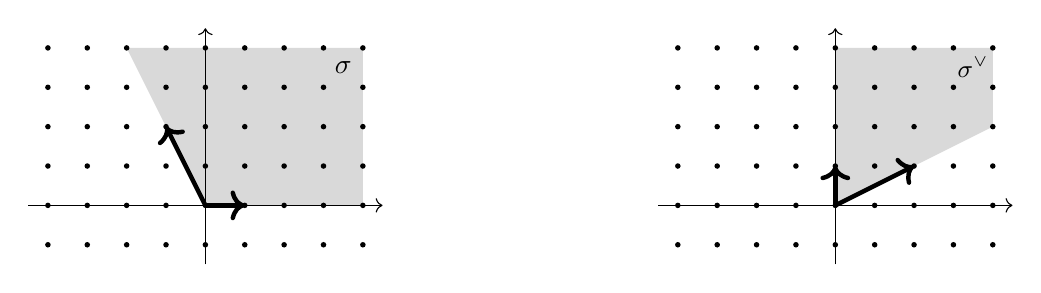
\begin{tikzpicture}
        % Left diagram
        \begin{scope}[shift={(-4,0)}]
            % Shaded area
            \fill[gray!30] (0,0) -- (-1,2) -- (2,2) -- (2,0) -- cycle;
            
            % Axes
            \draw[->] (-2.25,0) -- (2.25,0);
            \draw[->] (0,-0.75) -- (0,2.25);
            
            % Lattice points
            \foreach \x in {-2,-1.5,-1,-0.5,0,0.5,1,1.5,2}
                \foreach \y in {-0.5,0,0.5,1,1.5,2}
                    \fill (\x,\y) circle (1pt);

            % Vectors
            \draw[->, ultra thick] (0,0) -- (0.5,0);
            \draw[->, ultra thick] (0,0) -- (-0.5,1);
            \node at (1.75, 1.75) {$\sigma$};
        \end{scope}
        
        % Right diagram
        \begin{scope}[shift={(4,0)}]
            % Shaded area
            \fill[gray!30] (0,0) -- (0,2) -- (2,2) -- (2, 1) -- cycle;
            
            % Axes
            \draw[->] (-2.25,0) -- (2.25,0);
            \draw[->] (0,-0.75) -- (0,2.25);
            
            % Lattice points
            \foreach \x in {-2,-1.5,-1,-0.5,0,0.5,1,1.5,2}
                \foreach \y in {-0.5,0,0.5,1,1.5,2}
                    \fill (\x,\y) circle (1pt);

            % Vectors
            \draw[->, ultra thick] (0,0) -- (0,0.5);
            \draw[->, ultra thick] (0,0) -- (1,0.5);
            \node at (1.75, 1.75) {\small{$\sigma^\vee$}};
        \end{scope}
    \end{tikzpicture}
\end{figure}
\noindent
While $\{2 e_1^* + e_2^*, e_2^*\}$ generates $\sigma^\vee$ as a cone, it does not generate $S_\sigma$ as a semigroup, since not every element in $S_\sigma$ lies in $\Span_{\ZZ_{\ge 0}} \{2 e_1^* + e_2^*,  e_2^*\}$.
For example, $e_1^* + e_2^* \in S_\sigma$, but $e_1^* + e_2^* \notin \Span_{\ZZ_{\ge 0}} \{2 e_1^* + e_2^*,  e_2^*\}.$
However, $\{e_2^*, 2 e_1^* + e_2^*,  e_1^* + e_2^*\}$ generates $S_\sigma$.
Then,
\begin{align*}
	\qquad k[S_\sigma] = k[\chi^{e_2^*}, \chi^{2 e_1^* + e_2^*}, \chi^{e_1^* + e_2^*}] &= k[X_2, X_1^2 X_2, X_1 X_2] \cong k[X, Y, Z] / (X Y - Z^2),
\end{align*}
and
$$U_\sigma = \Spec(k[X, Y, Z] / (XY - Z^2) )= \bV(X Y - Z^2).$$

\item
Consider $\sigma = \Span_{\RR_{\ge 0}}\{ e_1, e_2, e_1+e_3, e_2 + e_3\}$ and $\sigma^\vee = \Span_{\RR_{\ge 0}} \{e_1^*, e_2^*, e_3^*, e_1^* +e_2^* - e_3^*\}.$
We have 
\begin{align*}
	k[S_\sigma] &= k[\chi^{e_1^*}, \chi^{e_2^*}, \chi^{e_3^*}, \chi^{e_1^* +e_2^* - e_3^*}] \\
	&= k[X_1, X_2, X_3, X_1 X_2 X_3^{-1}] \\
	&\cong k[X, Y, Z, W]/(XY - ZW),
\end{align*}
and so
$$U_\sigma = \Spec(k[X, Y, Z, W] / (XY - ZW) ) = \bV(XY-ZW).$$
\end{enumerate}
\end{example}





\subsection{Points of toric varieties}\label{section:points}
We have seen how points in affine varieties correspond to maximal ideals in the coordinate ring (cf.\ \S \ref{section:thenullstellensatz} and \S \ref{section:themaximalspectrum}).
Our goal in this section is to explain the different ways of viewing points in affine toric varieties.
The fact that the coordinate ring of an affine toric variety arises as a semigroup algebra affords us another perspective of points, namely as semigroup homomorphisms.
Later, in \S\ref{section:thetorusaction}, we will use the semigroup homomorphism point of view to define a torus action on an affine toric variety.

\begin{proposition}[{\cite[Proposition 1.3.1]{CLS11}}]\label{proposition:pointbijections}
Let $\sigma$ be a cone in $N$ and $U_\sigma = \Spec(k[S_\sigma])$ the associated affine toric variety.
The following sets are in bijection:
\begin{enumerate}
\item The set of points of $U_\sigma$.
\item The set of maximal ideals of $k[S_\sigma]$.
\item The set of $k$-algebra homomorphisms $k[S_\sigma] \to k$.
\item The set of semigroup homomorphisms $S_\sigma \to k$.\footnote{Here, $k$ is considered as a semigroup under multiplication.}
\end{enumerate}
\end{proposition}

\begin{proof}
The bijection between (1) and (2) holds by definition of the maximal spectrum.
We saw the bijection between (1) and (3) in Example \ref{example:pointsandhoms}.

We explain the bijection between (3) and (4) now.
Given a $k$-algebra homomorphism $\varphi : k[S_\sigma] \to k$, define a semigroup homomorphism $x : S_\sigma \to k$ by $x(u) := \varphi(\chi^u)$.
Conversely, a semigroup homomorphism $x : S_\sigma \to k$ determines a $k$-algebra homomorphism $\varphi : k[S_\sigma] \to k$, defined on basis elements by $\varphi(\chi^u) := x(u)$.
These maps are mutually inverse and are hence bijections.
\end{proof}

Let us take a closer look at the above bijections when $U_\sigma = T_N = U_{\{0\}}$.

\begin{example}
We saw in \S \ref{section:affinetoricvarieties} that when $\sigma = \{0\}$, the semigroup $S_\sigma$ is generated by $\pm e_1^*, \ldots, \pm e_n^*$, where $\{e_1^*, \ldots, e_n^*\}$ is a basis of $M$.
We write $X_i := \chi^{e_i^*}$ so that $k[S_\sigma] = k[X_1^{\pm}, \ldots, X_n^\pm]$.
We now detail the sets named in Proposition \ref{proposition:pointbijections}.
\begin{enumerate}
\item The set of points of $U_\sigma = (k^\times)^n$ is $\{(a_1, \ldots, a_n) : a_i \ne 0\}$ (when considering $(k^\times)^n$ embedded in $\AA^n$).
\item For brevity, let $A$ denote the polynomial ring $k[X_1, \ldots, X_n]$ and $h$ the element $X_1 \cdots X_n$.
We know $k[S_\sigma]$ is the localization $A_h$ (cf.\ \S\ref{section:opensubsetsofalgebraicsets}).
Maximal ideals in $A_h$ are all of the form $\frakm A_h$, where $\frakm$ is a maximal ideal of $A$ not containing $h$ (cf.\ Proposition \ref{proposition:localizationideals}).
The Nullstellensatz tells us every maximal ideal of $A$ is of the form $\frakm_a = (X_1 - a_1, \ldots, X_n - a_n)$ for some $a = (a_1, \ldots, a_n) \in \AA^n$.
One readily checks $\frakm_a$ does not contain $h$ if and only if each $a_i$ is non-zero.
Then the set of maximal ideals in $k[S_\sigma]$ is $$\{\frakm_a A_h : a = (a_1, \ldots, a_n) \in (k^\times)^n\}.$$
\item The $k$-algebra homomorphism $k[S_\sigma] \to k$ corresponding to the maximal ideal $\frakm_a$ is the unique map with kernel $\frakm_a$.
This map is defined on generators by $X_i^\pm \mapsto a_i^\pm$.
\item The semigroup homomorphism corresponding to the $k$-algebra homomorphism in (3) is
$$S_\sigma = M \to k, \qquad \pm e_i^* \mapsto a_i^\pm.$$
Note since $M$ is a group, every element in the image of a semigroup homomorphism $M \to k$ is invertible, and such a map is in fact a homomorphism of groups $M \to k^\times$.
\end{enumerate}
\end{example}

Let us consider how multiplication of points in $T_N = (k^\times)^n$ looks from the perspective of homomorphisms---this will be useful when defining the torus action in \S \ref{section:thetorusaction}.
Suppose $x : M \to k^\times$ and $y : M \to k^\times$ are homomorphisms given by $x(e_i^*) = a_i$ and $y(e_i^*) = b_i$.
Then $x$ and $y$ correspond to the points $(a_1, \ldots, a_n)$ and $(b_1, \ldots, b_n)$, respectively.
The product $(a_1 b_1, \ldots, a_n b_n)$ corresponds to the product of homomorphisms
$$xy : M \to k^\times, \qquad (xy)(e_i^*) := a_i b_i.$$




\subsection{Faces and open affine subsets}\label{section:facesandopenaffinesubsets}
In this section, we show how faces of a cone correspond to open affine subsets in an affine toric variety.
In particular, we will see that every affine toric variety contains a torus as a dense open subset.

If $\tau$ is a face of $\sigma$, then $\tau^\vee \supseteq \sigma^\vee$ and $S_\tau \supseteq S_\sigma$, since dualising reverses inclusion.
The inclusion of semigroups $S_\sigma \hookrightarrow S_\tau$ induces the inclusion of $k$-algebras $k[S_\sigma] \hookrightarrow k[S_\tau]$, and hence a morphism $U_\tau \to U_\sigma$ (cf.\ \S \ref{section:morphisms}).
The main result of this section is to show this morphism embeds $U_\tau$ as a principal open subset of $U_\sigma$.

\begin{proposition}\label{proposition:facesopensubsets}
If $\tau$ is a face of $\sigma$, then the map $U_\tau \to U_\sigma$ embeds $U_\tau$ as a principal open subset of $U_\sigma$.
\end{proposition}

The above proposition is one reason why we use dual cones to define toric varieties: smaller faces in a cone correspond to smaller open subsets in the variety.
In other words, using dual cones gives an inclusion-preserving correspondence between faces and open subsets.

Before proving Proposition \ref{proposition:facesopensubsets}, we consider some of its consequences:
\begin{enumerate}
\item The torus $T_N = U_{\{0\}}$ is a dense open subset of $U_\sigma$. The cone $\sigma$ is strongly convex so $\{0\}$ is a face. Then the proposition says $U_{\{0\}}$ is a principal open subset of $U_\sigma$, and open subsets of an irreducible affine variety are dense \cite[\S 4.2]{Reid88}.
\item The dimension of $U_\sigma$ is $\dim N_\RR = n$. We have $\dim U_\sigma = \dim T_N = n$, because the dimension of an open subset of an irreducible variety equals the dimension of the variety \cite[Chapter 5, j]{Milne23}.
\end{enumerate}
\noindent These important consequences rely on $\sigma$ being strongly convex, justifying why we make this assumption about our cones.

To prove Proposition \ref{proposition:facesopensubsets}, we start with a lemma that describes the relationship between the semigroups $S_\tau$ and $S_\sigma$, which elucidates the relationship between $k[S_\tau]$ and $k[S_\sigma]$.

\begin{lemma}
If $\tau$ is a face of $\sigma$, then $\tau = \sigma \cap u^\perp$ for some $u \in S_\sigma$.
Moreover, we have $S_\tau =S_\sigma + \ZZ_{\ge 0} \cdot (-u).$
\end{lemma}
\begin{proof}
By definition, $\tau = \sigma \cap u^\perp$ for some $u \in \sigma^\vee$, but we need to construct such a $u$ in the lattice to conclude $u \in S_\sigma$.
Notice $\sigma^\vee \cap \tau^\perp$ is a face in the rational cone $\sigma^\vee$, so there are $u_1, \ldots, u_s$ lying in the lattice which generate $\sigma^\vee \cap \tau^\perp$.
We define $u := \sum_{i=1}^s u_i \in S_\sigma$.
To see $\tau \subseteq \sigma \cap u^\perp$, observe that if $v$ lies in $\tau$, then $\langle u, v\rangle = 0$, since $u$ lies in $\sigma^\vee \cap \tau^\perp$.
Conversely, suppose $v$ lies in $\sigma \cap u^\perp$.
It follows $\langle u_i, v \rangle = 0$ for each $i$, and hence $v \in (\sigma^\vee \cap \tau^\perp)^\perp$.
Then $v$ lies in $\sigma \cap (\sigma^\vee \cap \tau^\perp)^\perp$, and Lemma \ref{lemma:dualfaces} implies  $\tau = \sigma \cap (\sigma^\vee \cap \tau^\perp)^\perp$.

To see $S_\tau \subseteq S_\sigma + \ZZ_{\ge 0} \cdot (-u)$, let $w \in S_\tau$, and suppose $v_1, \ldots, v_r$ lie in the lattice and generate $\sigma$ as a cone.
For any $v = \sum_{i=1}^r t_i v_i$ in $\sigma$ (where each $t_i \ge 0$) and any positive integer $p$, we have
$$\langle w + pu, v\rangle = \sum_{i=1}^r t_i \left( \langle w, v_i \rangle + p \langle u, v_i \rangle \right).$$
We want to choose $p$ so that each summand is non-negative to ensure $\langle w+pu, v \rangle \ge 0$.
For all $i$, there holds $\langle u, v_i \rangle \ge 0$.
Thus, when $\langle w, v_i \rangle \ge 0$, the $i^\text{th}$ summand is non-negative.
If $\langle w, v_i\rangle < 0$, then $v_i$ does not lie in $\tau$.
In this case, we must have $\langle u, v_i\rangle \ge 1$, because $v_i \notin \tau$ means $\langle u, v_i \rangle \ne 0$, and $\langle u, v_i \rangle$ lies in $\ZZ$ since $u$ and $v_i$ are both lattice points.
It follows that if $p := \max_i |\langle u, v_i\rangle|$, then each summand is non-negative.
Thus, $w + pu \in S_\sigma$ and $w \in S_\sigma + \ZZ_{\ge 0} \cdot (-u).$

Conversely, if $w - pu \in S_\sigma + \ZZ_{\ge 0} \cdot (-u)$, then for any $v \in \tau$, we have $\langle w - pu, v\rangle = \langle w, v \rangle \ge 0$, and so $w - pu \in S_\tau$.
\end{proof}

We are now ready to prove Proposition \ref{proposition:facesopensubsets}.

\begin{proof}[{Proof of Proposition \ref{proposition:facesopensubsets}}]
The lemma yields $u$ in $S_\sigma$ such that $\tau = \sigma \cap u^\perp$ and $S_\tau = S_\sigma + \ZZ_{\ge 0} \cdot (-u)$.
Then any basis element of $k[S_\tau]$ can be written $\chi^{w - pu} = \frac{\chi^w}{\chi^{pu}}$ for some $w \in S_\sigma$ and $p \in \ZZ_{\ge 0}$.
It follows that $k[S_\tau]$ is the localization $k[S_\sigma]_{\chi^u}$, and the inclusion $k[S_\sigma] \hookrightarrow k[S_\tau] = k[S_\sigma]_{\chi^u}$ is the localization homomorphism.
Proposition \ref{proposition:localizationembedding} tells us that the corresponding morphism $U_\tau \to U_\sigma$ embeds $U_\tau$ as a principal open subset of $U_\sigma$.
\end{proof}

\subsection{The torus action}\label{section:thetorusaction}
In this section, we define an action of the dense torus on an affine toric variety.
This means the affine toric varieties we have defined in terms of cones are toric varieties in the sense mentioned in the introduction to this chapter.
The torus action is defined using the semigroup homomorphism perspective of points.
Afterwards, we check this defines a group action which extends the natural action of a torus on itself.
We conclude the section with examples.

Let $\sigma$ be a cone in $N$.
We refer to semigroup homomorphisms as points, using the identification established in \S\ref{section:points}.
Let $t : M \to k^\times$ and $x : S_\sigma \to k$ be points in $T_N$ and $U_\sigma$, respectively.
The action map $\varphi : T_N \times U_\sigma \to U_\sigma$ is defined by 
$$(t, x) \mapsto (u \mapsto t(u)x(u)).$$
We write $t \cdot x$ for the image of $(t, x)$.
Then $t \cdot x$ is simply the product of semigroup homomorphisms.
We now prove $\varphi$ is a group action extending the natural action of $T_N$ on itself.

\begin{proposition}
The map $\varphi : T_N \times U_\sigma \to U_\sigma$ is a group action.
Moreover, under the identification of $T_N$ with an open subset of $U_\sigma$, $\varphi$ extends the natural action of $T_N$ on itself by left multiplication.
\end{proposition}
\begin{proof}
To prove $\varphi$ is an action of the algebraic group $T_N$, we must show $\varphi$ is a morphism of varieties and also a group action.

To see $\varphi$ is a morphism, we check its pullback is a $k$-algebra homomorphism.
To evaluate the regular function $\chi^u \in k[S_\sigma]$ at $x : S_\sigma \to k$, we compute $\chi^u(x) = x(u)$ (cf.\ Example \ref{example:pointsandhoms} and Proposition \ref{proposition:pointbijections}).
We see
$$\varphi^*(\chi^u)(t, x) = \chi^u(t\cdot x) = (tx)(u) = (\chi^u \otimes \chi^u)(t,x).$$
Then $\varphi^* : k[S_\sigma] \to k[M] \otimes k[S_\sigma]$ is given by $\chi^u \mapsto \chi^u \otimes \chi^u$, which is clearly a homomorphism.

The semigroup homomorphism corresponding to the identity in $T_N$ is the trivial homomorphism $1_{T_N} : M \to k^\times$.
Using this, and the fact that the product in $T_N$ is given by the product of semigroup homomorphisms (cf.\ \S \ref{section:points}), it is straightforward to check $1 \cdot x = x$ and $t_1\cdot(t_2\cdot x) = (t_1t_2)\cdot x$.
Then $\varphi$ is a group action.

We also need to check this action extends the natural action of $T_N$ on itself by left multiplication.
From \S\ref{section:facesandopenaffinesubsets}, we have a map $\iota : T_N \hookrightarrow U_\sigma$ embedding $T_N$ as an open subset of $U_\sigma$.
We need to check $t_1 \cdot \iota(t_2) = \iota(t_1 t_2)$ for any two points $t_1$ and $t_2$ in $T_N$.
Since the action is defined using semigroup homomorphisms, we need to understand $\iota$ at the level of semigroup homomorphisms.
If $t : M \to k^\times$ is a point in $T_N$, then $\left. t \right|_{S_\sigma} : S_\sigma \to k$ is a point in $U_\sigma$.
This is a natural guess for how $\iota$ is evaluated on semigroup homomorphisms.
Evaluating this restriction map at $t : M \to k^\times$, then applying a regular function $\chi^u \in k[S_\sigma]$, gives
$$\chi^u(\left. t \right|_{S_\sigma}) = \left. t \right|_{S_\sigma}(u) = t(u) = \chi^u(t).$$
This agrees with $\iota^*(\chi^u)(t)$, so our guess is correct.
Then $t_1 \cdot \iota(t_2)$ and $\iota(t_1 t_2)$ both equal $\left. t_1 t_2 \right|_{S_\sigma}$.
\end{proof}

We now examine this torus action for the toric varieties we saw in Example \ref{example:affinetoricvarieties}.

\begin{example}
\begin{enumerate}
\item Consider $\sigma = \Span_{\RR_{\ge 0}}\{e_1, \ldots, e_n\}$ and $S_\sigma = \Span_{\ZZ_{\ge 0}}\{e_1^*, \ldots, e_n^*\}$.
Then a semigroup homomorphism $x : S_\sigma \to k$ is given by $e_i^* \mapsto a_i$ for some $(a_1, \ldots, a_n) \in \AA^n$.
Points in the torus $t : M \to k^\times$ are given by $e_i^* \mapsto b_i$ for some $(b_1, \ldots, b_n)\in(k^\times)^n$.
We then see the embedding of $T_N$ into $\AA^n$ is the usual one.
The torus action is given by $t\cdot x : S_\sigma \to k$, where $e_i^* \mapsto a_i b_i$, so $T_N$ acts on $\AA^n$ by component-wise multiplication.
\item Consider $\sigma = \Span_{\RR_{\ge 0}} \{e_1, -e_1 + 2 e_2\}$ and $S_\sigma = \Span_{\ZZ_{\ge 0}}\{e_2^*, 2e_1^*+e_2^*, e_1^*+e_2^*\}$.
Any point in $U_\sigma = \bV(XY- Z^2)$ is a map $p : S_\sigma \to k$, given on the generators by
$$e_2^* \mapsto x, \qquad 2e_1^*+e_2^* \mapsto y, \qquad e_1^*+e_2^* \mapsto z,$$
subject to the restraint $xy=z^2$ so that the map is a homomorphism.
A point in the torus $T_N = (k^\times)^2$ is a map $t : M \to k^\times$ given by
$$e_1^* \mapsto a, \qquad e_2^* \mapsto b.$$
The restriction $\left. t \right|_{S_\sigma}$ gives the embedding $T_N \hookrightarrow U_\sigma$.
This is the homomorphism $\left. t \right|_{S_\sigma} : S_\sigma \to k$ given by
$$e_2^* \mapsto b, \qquad 2e_1^*+e_2^* \mapsto a^2 b, \qquad e_1^*+e_2^* \mapsto ab.$$
We see the embedding $T_N \hookrightarrow U_\sigma$ is given by $(a, b) \mapsto (b, a^2 b, ab)$.
This means $T_N$ is all the points in $U_\sigma$ with non-zero coordinates.
Furthermore, $t\cdot p = tp : S_\sigma \to k$ is given by
$$e_2^* \mapsto bx, \qquad 2e_1^*+e_2^* \mapsto a^2 by, \qquad e_1^*+e_2^* \mapsto abz.$$
In other words, the action can be written explicitly as
$$(b, a^2b, ab) \cdot (x, y, z) = (bx, a^2by, abz).$$
\end{enumerate}
\end{example}


\subsection{Singularities}
In this section, we characterise when affine toric varieties are non-singular using their cones.

\begin{theorem}\label{theorem:singularities}
An affine toric variety $U_\sigma$ is non-singular if and only if $\sigma$ is generated by a subset of a basis for the lattice $N$.
In this case,
$$U_\sigma \cong k^r \times (k^\times)^{n-r},$$
where $r = \dim(\sigma)$.
\end{theorem}

We have already seen that $U_\sigma$ is isomorphic to $k^r \times (k^\times)^{n-r}$ when $\sigma$ is generated by $r$ basis vectors of $N$ (cf.\ Example \ref{example:affinetoricvarieties}).
Therefore, it remains to prove the converse.
To do so, we need to consider the so-called distinguished point $x_\sigma$ in $U_\sigma$.
This point is given by the map of semigroups
$$x_\sigma : S_\sigma \to k, \qquad x_\sigma(u) := \begin{cases} 1 & \text{if } u \in \sigma^\perp, \\ 0 & \text{otherwise.} \end{cases}$$
This is a homomorphism since $\sigma^\perp$ is a face of $\sigma^\vee$, so a sum of two elements in $S_\sigma$ lies in $\sigma^\perp$ if and only if each element lies in $\sigma^\perp$ \cite[\S 2.1]{Fulton93}.
The strategy of the proof of Theorem \ref{theorem:singularities} is to show that if $U_\sigma$ is non-singular at $x_\sigma$, then $\sigma$ is generated by a subset of a basis for $N$.

\begin{proof}
We consider the case when $\sigma$ is non-degenerate. For a proof of the degenerate case, see \cite[\S 2.1]{Fulton93}.

As $\sigma$ spans $N_\RR$, we have $\sigma^\perp = \{0\}$.
Thus, $x_\sigma(u)$ equals 1 if $u=0$ and equals 0 if $u \ne 0$.
The maximal ideal $\frakm$ corresponding to $x_\sigma$ is the ideal of regular functions vanishing at $x_\sigma$.
As $\chi^u(x_\sigma) = x_\sigma(u)$, we see $\frakm$ is generated by the $\chi^u$ for all $u \in S_\sigma \setminus \{0\}$.
Hence, $\frakm^2$ is generated by the $\chi^u$ such that $u$ is a sum of two elements in $S_\sigma \setminus \{0\}$.
We see $\frakm / \frakm^2$ has the basis 
$$\{\chi^u + \frakm^2 : u \in (S_\sigma)_{\text{irred}}\},$$
where $(S_\sigma)_{\text{irred}}$ is the set
$$(S_\sigma)_{\text{irred}} = \{u \in S_\sigma \setminus \{0\} : u \text{ is not a sum of two elements in } S_\sigma\setminus\{0\}\}.$$
Since $U_\sigma$ is non-singular, the Zariski tangent space $(\frakm/\frakm^2)^*$ has dimension $n = \dim(U_\sigma)$, and thus $|(S_\sigma)_{\text{irred}}| = n$.

We now consider which elements lie in $(S_\sigma)_{\text{irred}}$.
Any edge (i.e., a one-dimensional face) of $\sigma^\vee$ can be generated by a single lattice element.
If $p u$ lies in $S_\sigma$ for some $p \in \ZZ_{> 0}$ and $u \in M$, then $u$ lies in $S_\sigma$, since $S_\sigma$ is the intersection of $M$ with a cone.
Then for any edge, there exists a unique $u \in S_\sigma$ generating the edge which is not the sum of two non-zero elements in the edge.
Such a $u$ is called a minimal edge generator.
The minimal edge generators lie in $(S_\sigma)_{\text{irred}}$ \cite[Proposition 1.2.23]{CLS11} and generate the cone \cite[Lemma 1.2.15]{CLS11}.
Since $\sigma$ is strongly convex, $\sigma^\vee$ spans $M_\RR$ and there must be $n$ minimal edge generators.
We conclude $(S_\sigma)_{\text{irred}}$ is the set of minimal edge generators.

Then $(S_\sigma)_{\text{irred}}$ is a set of $n$ linearly independent lattice points that generate the cone.
To complete the proof, we just need to show $(S_\sigma)_{\text{irred}}$ generates $M$ as a group.
This follows from two facts: $(S_\sigma)_{\text{irred}}$ generates $S_\sigma$ \cite[Proposition 1.2.23]{CLS11}, and $S_\sigma + (-S_\sigma) = M$.
The latter is true because $\sigma^\vee$ spans $M_\RR$.
\end{proof}

We revisit the singular affine toric varieties we saw in Example \ref{example:affinetoricvarieties} to see how the cone generators detect when the variety is singular.

\begin{example}
\begin{enumerate}
\item If $\sigma = \Span_{\RR_{\ge 0}}\{e_1, e_2, e_1+e_3, e_2+e_3\}$, then $U_\sigma = \bV(XY - ZW).$
Note $U_\sigma$ is singular since all partial derivatives of $XY-ZW$ vanish at the origin.
The generating set $\{e_1, e_2, e_1+e_3, e_2+e_3\}$ is not a basis for $\ZZ^3$ as it contains four vectors.
\item If $\sigma = \Span_{\RR_{\ge 0}}\{e_1, -e_1+2e_2\}$, then $U_\sigma = \bV(XY - Z^2).$
Again, $U_\sigma$ is singular since all partial derivatives of $XY-Z^2$ vanish at the origin.
Notice that any point in the $\ZZ$-span of the generating set $\{e_1, -e_1+2e_2\}$ has even $y$-component; thus, the generating set is not a basis for $\ZZ^2$.
\end{enumerate}
\end{example}










\newpage
\section{Torus quotients as toric varieties}\label{chapter:gitquotientsastoricvarieties}
In this chapter, we prove the main theorem of this thesis.
We show that when $V$ is a rational representation of a torus $T$, the GIT quotient $V \git T$ is a toric variety.
To prepare for the proof, we define algebraic groups, and their actions and representations in \S \ref{section:algebraicgroups}.
Next, we define the GIT quotient in \S \ref{section:gitquotient}.
In \S \ref{section:invariantsoftorus}, we compute the invariant ring for the action of $T$ on $V$.
Following this, we can prove the main theorem in \S \ref{section:torusquotientsastoricvarieties}.
To conclude the thesis, in \S \ref{section:examples}, we compute examples of the cone corresponding to the toric variety $V \git T$.





\subsection{Algebraic groups and their actions}\label{section:algebraicgroups}
In this section, we introduce the theory of algebraic groups necessary for defining the GIT quotient in \S \ref{section:gitquotient}.
We first define algebraic groups, their actions, and representations.
Following this, we discuss classic invariant theory and the problem of finite generation of invariants.
Useful references for this material include \cite{Humphreys75}, \cite{Geck13}, \cite{Springer98}, and \cite{Mukai03}.

Let $G$ be an (affine) variety which is also a group.
Consider the multiplication map $\mu : G \times G \to G$ defined by $(x, y) \mapsto xy$, and the inversion map $\iota : G \to G$ defined by $x \mapsto x^{-1}$.
If $\mu$ and $\iota$ are morphisms of varieties, we say $G$ is an \emph{(affine) algebraic group}.
A map between algebraic groups $\varphi : G \to G'$ is called a \emph{homomorphism of algebraic groups} if it is a group homomorphism and a morphism of varieties.
An \emph{isomorphism} is a homomorphism which is an isomorphism of groups and varieties.
We say $H$ is a \emph{closed subgroup} of $G$ if it is a subgroup of $G$ and closed in the Zariski topology;
closed subgroups are algebraic groups in their own right, and the inclusion $H \hookrightarrow G$ is a homomorphism of algebraic groups.

We now detail examples of algebraic groups and closed subgroups.

\begin{example}
\begin{enumerate}
\item The additive group $\GG_a$ is the algebraic group with underlying variety $\AA^1$, multiplication map $\mu(x, y) = x + y$, and inversion map $\iota(x) = - x$. 
\item The multiplicative group $\GG_m$ is the algebraic group with underlying variety $k^\times$, multiplication map $\mu(x, y) = xy$, and inversion map $\iota(x) = x^{-1}$.
\item Recall the general linear group $\GL_n(k)$ is the group of $n \times n$ invertible matrices with entries in $k$.
When $\AA^{n \times n}$ is identified with the set of all $n \times n$ matrices, $\GL_n(k)$ is the principal open subset where $\det \ne 0$.
Thus, $\GL_n(k)$ is an affine variety (cf.\ Proposition \ref{proposition:localizationembedding}).
Its coordinate ring is the localization $k[\AA^{n \times n}]_{\det}$.
If $A, B \in \GL_n(k)$, then the entries of $AB$ are polynomials in the entries of $A$ and $B$, so $\mu$ is a morphism. 
The inversion map $\iota$ is a morphism by Cramer's rule, as entries of $A^{-1}$ are polynomials in the entries of $A$ and $\frac{1}{\det(A)}$.
\item An algebraic group we saw in Chapter \ref{chapter:affinetoricvarieties} is the $n$-dimensional algebraic torus $T = (k^\times)^n$.
This is isomorphic to the closed subgroup of diagonal matrices in $\GL_n(k)$, which is denoted $D_n(k)$.
If $X_{ij}$ denote the coordinate functions on $\GL_n(k)$, then $D_n(k)$ is the closed subset defined by the equations $X_{ij} = 0$ for all $i \ne j$.
The map $T \to D_n(k)$ given by $(t_1, \ldots, t_n) \mapsto \diag(t_1, \ldots, t_n)$ is an isomorphism of algebraic groups.
\item Important algebraic groups arising as closed subgroups of $\GL_n(k)$ include the special linear group $\SL_n(k)$, the special orthogonal group $\SO_n(k)$ and the symplectic group $\Sp_{2n}(k)$ \cite[\S 1.3]{Geck13}.
\end{enumerate}
\end{example}

We now detail examples of morphisms of algebraic groups.

\begin{example}\label{example:algebraicgroupmorphisms}
\begin{enumerate}
\item The determinant map $\det : \GL_n(k) \to \GG_m$ is a morphism of algebraic groups:
it is a morphism since $\det(A)$ is a polynomial in the entries of $A$, and a homomorphism since $\det(AB)=\det(A)\det(B)$.
\item We now classify algebraic group morphisms $\varphi : \GG_m \to \GG_m$.
These correspond to algebra endomorphisms $\varphi^* : k[T, T^{-1}] \to k[T, T^{-1}]$ (cf.\ Proposition \ref{proposition:morphismsandhomomorphism}).
It can be shown that the units in $k[T,T^{-1}]$ are $\{u T^n : u \in k^\times, n \in \ZZ\}$, so since $\varphi^*(T)\varphi^*(T^{-1}) = 1$, we must have $\varphi^*(T) = u T^n$ for some $u \in k^\times$ and $n \in \ZZ$.
The endomorphism $\varphi^*(T) = u T^n$ corresponds to the morphism $\varphi(t) = u t^n$.
Since $\varphi$ is a group homomorphism, we must have $u =1$.
Therefore, $\Hom(\GG_m, \GG_m) = \{t \mapsto t^n : n \in \ZZ\}\cong\ZZ.$
\end{enumerate}
\end{example}

We can now define actions and representations of algebraic groups.
Before doing so, we recall the definitions of group actions and group representations for a general group $G$.
An action of $G$ on a set $S$ is a map $\cdot : G \times S \to S$, $(g, s) \mapsto g \cdot s$, such that $1 \cdot s = s$ and $g \cdot (h \cdot s) = (g\cdot h) \cdot s$ for all $g$ and $h$ in $G$.
A representation is a linear action of $G$ on a vector space $V$, or equivalently, a group homomorphism $G \to \GL(V)$.

Now suppose $G$ is an algebraic group and $V$ is an affine variety.
An \emph{algebraic group action} of $G$ on $V$ is a morphism of varieties $\varphi : G \times V \to V$ that is also a group action.

Suppose that $V$ is a finite dimensional $k$-vector space.
Let $\rho : G \to \GL(V)$ be a homomorphism of abstract groups.
After choosing a basis for $V$, the map $\rho$ can be viewed as a homomorphism $G \to \GL_n(k)$.
We say $\rho$ is a \emph{rational representation} of $G$ if the entries of $\rho(g) \in \GL_n(k)$ lie in the coordinate ring $k[G]$.
Different bases differ by linear transformations, so the definition is independent of the choice of basis.

Examples of algebraic group actions will follow our discussion of invariant theory (cf.\ Example \ref{example:invariantrings}).

We now define the characters of an algebraic group $G$.
These can be viewed as the one-dimensional rational representations, and play an important role in \S \ref{section:invariantsoftorus} and \S \ref{section:torusquotientsastoricvarieties}.
A \emph{character} of $G$ is an algebraic group homomorphism $G \to \GG_m \cong \GL_1(k)$.
The set of all characters of $G$ defines a group under pointwise multiplication. 
This group is called the \emph{character group} of $G$, and is denoted $X^*(G)$.
Since $X^*(G)$ is abelian, we write its operation additively:
$$(\chi_1+\chi_2)(g) := \chi_1(g)\chi_2(g)$$
for all $\chi_1, \chi_2 \in X^*(G)$ and $g \in G$.
The identity character (denoted 0), maps all elements to 1.

We now compute the character group of a torus, following \cite[Example 3.1.4]{Geck13}.

\begin{example}
Example \ref{example:algebraicgroupmorphisms} shows $X^*(\GG_m)=\Hom(\GG_m,\GG_m)\cong\ZZ$.
If $T = \GG_m^n$ is the $n$-dimensional torus, then $X^*(T) \cong \ZZ^n$.
This follows from the fact that if $G_1$ and $G_2$ are any algebraic groups, then the map $X^*(G_1)\times X^*(G_2) \to X^*(G_1\times G_2)$ given by $(\chi_1, \chi_2) \mapsto ((g_1, g_2) \mapsto \chi_1(g_1)\chi_2(g_2))$ is an isomorphism.
We call $X^*(T)$ the \emph{character lattice} of $T$ since it is a finitely generated free abelian group.
We can explicitly give an isomorphism $\ZZ^n \to X^*(T)$.
Let $\chi_i$ be the character of $T$ defined by $\chi_i(t_1, \ldots, t_n) := t_i$.
The map $\ZZ^n \to X^*(T)$ given by $e_i \mapsto \chi_i$ is an isomorphism of abelian groups;
in particular, $\{\chi_1, \ldots, \chi_n\}$ is a basis of $X^*(T)$.
\end{example}

We now turn to classical invariant theory.
We will discuss rings of invariants, and in particular, when these are finitely generated.
For further details, see \cite{FSR17} or \cite{Mukai03}.

Suppose that $G$ is an algebraic group acting on an affine variety $V = \Spec(A)$, where $A$ is a finitely generated reduced $k$-algebra.
There is an induced action on $A$, given by
$$(g \cdot f)(P) := f(g^{-1} \cdot P).$$
The \emph{ring of invariants} is
$$A^G := \{f \in A : g \cdot f = f \text{ for all } g \in G\}.$$

In the late nineteenth century, invariant theorists studied $A^G$ in the case when $V$ is a vector space (in which case, $A$ is the ring of polynomial functions on $V$) \cite{DC70}.
An important problem in classical invariant theory is to determine when $A^G$ is finitely generated.
For example, in 1868, Gordan computed a finite set of generators when $\SL_2(\CC)$ acts on the vector space of two variable homogeneous polynomials.
In 1890, Hilbert showed that if $V$ is a finite-dimensional representation of $G = \SL_n(\CC)$, then $A^G$ is finitely generated.

In fact, Hilbert's 1890 proof shows that the invariants of any representation of a \emph{reductive} group are finitely generated \cite[\S 3.1]{DC70}.
A group is reductive if it is connected and has trivial \emph{unipotent radical} \cite[\S 19.5]{Humphreys75}.
Examples of reductive groups include $\GL_n(k)$, $\SL_n(k)$, and tori.

When Mumford developed the theory of GIT in the 1960s, he was interested in the conditions under which $A^G$ is finitely generated for an arbitrary algebraic variety $V$.
He conjectured $A^G$ is always finitely generated for reductive groups \cite{Mumford65}.
Nagata proved that $A^G$ is finitely generated for so-called \emph{geometrically reductive} groups.
Later, Haboush proved that the notions of reductivity and geometric reductivity are equivalent for groups defined over a field of characteristic zero, thereby proving Mumford's conjecture in the characteristic zero case \cite[\S 12.1]{FSR17}.
The upshot is that when $G$ is reductive, $A^G$ is the coordinate ring of an affine variety---this will be important in \S \ref{section:gitquotient}.

To conclude this section, we provide examples of rings of invariants.

\begin{example}\label{example:invariantrings}
\begin{enumerate}
\item
Consider the group $G = k^\times$ acting on $V = \AA^2$ by 
$$t \cdot (x, y) = (tx, t^{-1}y).$$
We can write a polynomial $p \in k[X,Y]$ as $p = \sum_{i, j} p_{ij} X^i Y^j$, where the sum is over all positive integers $i$ and $j$ and all but finitely many coefficients $p_{ij}$ are zero.
Then $p$ is $k^\times$-invariant if and only if for all $t \in k^\times$,
$$\sum_{i, j} p_{ij} X^i Y^j = \sum_{i, j} p_{ij} t^{i-j} X^i Y^j.$$
This is equivalent to having $p_{ij} \ne 0$ if and only if $i = j$.
Thus, we have that
$$k[X, Y]^{k^\times} = \CC[XY].$$

\item
Consider $G = \GL_2(k)$ acting on its Lie algebra $\frakg = \frakg\frakl_2(k)$ by conjugation.
We know from linear algebra that the trace and determinant of a matrix are invariant under conjugation, so $\tr, \det \in k[\frakg]^G$.
In fact, $\tr$ and $\det$ generate the invariant ring and are algebraically independent \cite[Example 44]{Kamgarpour21}.
We conclude that the invariant ring is the free polynomial ring
$$k[\frakg]^G = k[\tr, \det].$$

\item
Consider $G = S_2 = \{1, \sigma\}$ acting on $V = \AA^2$ by
$$\sigma \cdot (x, y) = (-x, -y).$$
Then $p = \sum_{i, j} p_{ij} X^i Y^j \in k[X, Y]$ is $S_2$-invariant if and only if
$$\sum_{i, j} p_{ij} X^i Y^j = \sum_{i, j} p_{ij} (-1)^{i+j} X^i Y^j.$$
The above equality holds if and only if $i + j$ is even whenever $p_{ij}\ne 0$.
Any monomial $X^iY^j$ such that $i+j$ is even is a product of the monomials $X^2, XY$ and $Y^2$.
Thus,
$$k[X, Y]^{S_2} = k[X^2, XY, Y^2] \cong k[A, B, C]/(B^2 - AC).$$
\end{enumerate}
\end{example}





\subsection{The affine GIT quotient}\label{section:gitquotient}
In this section, we define affine GIT quotients and explain some of their properties.
We first explain the problem of constructing quotient varieties.
Next, we provide an example of a specific quotient.
The example motivates the definition of the GIT quotient that follows.
Our exposition in this section follows \cite[\S 5.1]{Mukai03}.

Suppose $G$ is an algebraic group acting on an affine variety $V$.
A quotient variety is a variety $W$ with a quotient morphism $\pi : V \to W$.
In order to identify $W$ with the set of orbits $X / G$, we want each fibre of $\pi$ to be a unique $G$-orbit.

It is not always possible to construct a quotient $(W, \pi)$.
Nonetheless, we now explain one approach to do so.
First, the morphism $\pi$ must be constant on $G$-orbits, i.e., $G$-invariant.
One way to construct $G$-invariant maps is as follows:
if $f_1, \ldots, f_m$ are invariant functions in $k[V]^G$, then the map $\pi : V \to \AA^m$ defined by
$$x \mapsto (f_1(x), \ldots, f_m(x))$$
is $G$-invariant.
We can choose $f_1, \ldots, f_m$ to be generators for $k[V]^G$ and define $W$ to be the image $\pi(V)$.
There are two potential problems to keep in mind: it is not clear distinct orbits in $V$ map to distinct points in $W$, and the image $\pi(V)$ is not necessarily a variety since the image of a morphism need not be a variety (cf.\ Example \ref{example:polynomialmaps}).

We now detail an example of constructing a quotient using the method described above.
Let $G = \GG_m $ act on $V = \AA^2$ by
$$t \cdot (x, y) := (tx, t^{-1}y)$$
for $t \in G$ and $(x, y) \in V$.
We have the following orbits:
\begin{enumerate}
\item the origin $\{(0, 0)\}$;
\item the $x$-axis without the origin $k^\times \times \{0\}$;
\item the $y$-axis without the origin $\{0\} \times k^\times$;
\item hyperbolas $\{(x, y) \in \AA^2 : xy = c\}$, one orbit for each $c \in k^\times$. 
\end{enumerate}	
We have seen the ring of invariants for this action is
$$k[X,Y]^{\GG_m} = k[XY].$$
We define the map $\pi : \AA^2 \to \AA^1$ by
$$(x, y) \mapsto xy.$$
If we think of $\AA^2$ as $\Spec(k[X, Y])$ and $\AA^1$ as $\Spec(k[XY])$, then the above morphism arises from the inclusion of the invariant ring $k[XY]$ into $k[X, Y]$.
We see $\pi$ is surjective and in particular has the variety $\AA^1$ as its image.
The fibre over $c \ne 0$ is the orbit
$$\pi^{-1}(c) = \{(x, y) \in \AA^2 : xy = c\},$$
while the fibre over $0$ is the union of orbits
$$\pi^{-1}(0) = \{(0, 0)\} \cup k^\times \times \{0\} \cup \{0\} \times k^\times.$$
Then different orbits map to the same point in the quotient.
It is important to note, however, each fibre contains a unique closed orbit: $\pi^{-1}(c)$ is closed for $c \ne 0$, and $\{(0, 0)\}$ is the only closed orbit contained in $\pi^{-1}(0)$.

Although we would like fibres of the quotient morphism to be unique $G$-orbits, the above example demonstrates this may not be possible.
The map $\pi$ is continuous, so each fibre is a closed set.
Therefore, any orbit of the action which is not closed cannot be a fibre of the quotient map.
Then we cannot construct a quotient with the properties we described at the start of the section.

The affine GIT quotient provides one way to construct quotients with desirable properties.
We now give the definition:

\begin{definition}
Let $G$ be an algebraic group acting on an irreducible affine variety $V = \Spec(A)$.
The affine GIT quotient is the affine variety
$$V \git G := \Spec(A^G).$$
\end{definition}

The inclusion $A^G \hookrightarrow A$ determines a morphism of affine varieties
$$\pi : V \to V \git G,$$
which we call the affine quotient map.
The key properties of the quotient $V \git G$ are summarised in the following theorem.
To state the theorem, we need the following definition:
two $G$-orbits $\calO$ and $\calO'$ are called closure-equivalent if there exists a sequence of orbits $\calO = \calO_1, \calO_2, \ldots, \calO_{n-1}, \calO_n = \calO'$ such that the intersection of closures $\overline{\calO_i} \cap \overline{\calO_{i+1}}$ is non-empty for each $i=1, \ldots, n-1$.
Since the affine quotient map is continuous it takes the same value on closure-equivalent orbits.

\begin{theorem}\label{theorem:gittheorem}
If $G$ is a reductive group acting on an affine variety $X$, then the affine quotient map
$$\pi : V \to V \git G$$
is surjective and gives a one-to-one correspondence between points of $V \git G$ and closure-equivalence classes of $G$-orbits in $V$.
Each closure-equivalence class contains exactly one closed orbit, so points in $V \git G$ are in bijection with closed $G$-orbits.
\end{theorem}
\begin{proof}
See \cite[\S 5.1]{Mukai03}, in particular, Theorem 5.9 and Corollary 5.5.
\end{proof}

We now examples of the GIT quotients of the group actions studied in Example \ref{example:invariantrings}.

\begin{example}\label{example:gitquotients}
\begin{enumerate}
\item 
Consider $G = \GL_2(k)$ acting on its Lie algebra $\frakg = \frakg\frakl_2(k)$ by conjugation.
We saw $k[\frakg]^G = k[\tr, \det]$, and $\tr$ and $\det$ are algebraically independent.
Then, 
$$\frakg \git G = \Spec(k[\tr, \det]) = k^2.$$
The affine quotient map $\pi : \frakg \to k^2$ is given by $A \mapsto (\tr A, \det A).$

\item
Consider $G = S_2 = \{1, \sigma\}$ acting on $V = \AA^2$ by $\sigma \cdot (x, y) = (-x, -y)$.
We saw that $k[X, Y]^{S_2} = k[X^2, XY, Y^2] \cong k[A, B, C]/(B^2 - AC).$
Then, we have
$$\AA^2 \git S_2 = \Spec(k[X^2, XY, Y^2]) \cong \bV(B^2 - AC).$$
Note $\AA^2 \git S_2$ is singular, because all partial derivatives of $B^2 - AC$ vanish at the origin.
The affine quotient map $\pi : \AA^2 \to \bV(B^2 - AC)$ is given by $(x, y) \mapsto (x^2, xy, y^2).$
\end{enumerate}
\end{example}










\subsection{Invariants of a linear torus action}\label{section:invariantsoftorus}
Let $V$ be a rational representation of $T$.
The goal of the next two sections is to prove that the GIT quotient $V \git T$ is an affine toric variety.
To understand $V \git T$, in this section, we compute the ring of invariants $k[V]^T$.
In particular, we show $k[V]^T$ is isomorphic to a semigroup algebra $k[\calM]$.
In the next section, we use this to show $V \git T$ is a toric variety.

We first find a basis to identify $V$ with $\AA^n$.
Rational representations of tori are well-understood; the following lemma says $V$ is a direct sum of one-dimensional representations, providing a natural choice of basis for $V$:

\begin{lemma}
The representation $V$ is a direct sum of one-dimensional representations.
In each one-dimensional subspace, $t \in T$ acts by multiplication by $\chi(t)$, where $\chi$ is some character of $T$.
\end{lemma}
\begin{proof}
See \cite[3.2.3]{Springer98}.
\end{proof}

If the subspace
$$V_\chi = \{v \in V : t \cdot v = \chi(t) v \text{ for all } t \in T\}$$
is non-zero, we call $\chi$ a weight of the representation $V$ \cite[7.1.1]{Springer98}.
If $\chi$ is weight of $V$, then the subspace $V_\chi$ is called a weight space.
Note weight spaces may have dimension greater than one; the dimension of $V_\chi$ is called the multiplicity of the weight $\chi$.

Let $\chi_1, \ldots, \chi_n$ be the weights of $V$, counted with multiplicity. 
By combining bases for each weight space, we obtain a basis $\{v_1, \ldots, v_n\}$ for $V$ where each $v_i$ lies in $V_{\chi_i}$.
Every $v \in V$ is uniquely written $v = \sum_{i=1}^n z_i v_i$ for some $z_i \in k$, and since the action of $T$ is linear, 
$$t \cdot v = \sum_{i=1}^n \chi_i(t) z_i v_i.$$
We identify $V$ with the affine variety $\AA^n$ by the map
$$\sum_{i=1}^n z_i v_i \mapsto (z_1, \ldots, z_n).$$

To compute $k[V]^T$, we establish notation for polynomials in $k[V]$.
Suppose $v = \sum_{i=1}^n z_i v_i$ is an element of $V$.
For each $i=1, \ldots, n$, we define the dual basis vectors $Z_i : V \to k$ by
$$Z_i(v) = z_i.$$
Then the coordinate ring of $V$ is $k[V] = k[Z_1, \ldots, Z_n]$.
We write polynomials in $k[V]$ in the following way.
Given $\mu = (\mu_1, \ldots, \mu_n) \in \ZZ_{\ge 0}^n$, define the monomial
$$Z^\mu := \prod_{i=1}^n Z_i^{\mu_i},$$
so that we may write a polynomial $f \in k[V]$ as
$$f = \sum_\mu f_\mu Z^\mu, \qquad \text{for some } f_\mu \in k.$$
Here, the sum is over all $\mu \in \ZZ_{\ge 0}^n$, and all but finitely many coefficients $f_\mu \in k$ are zero.

We are now ready to compute the invariant ring $k[V]^T$.
Recall that the action of $T$ on $V$ induces an action of $T$ on $k[V]$, given by
$$(t \cdot f)(v) := f(t^{-1} \cdot v)$$
for $t \in T$, $f \in k[V]$ and $v \in V$.
We use this to determine the $T$-invariant polynomials.
Write $v =\sum_{i=1}^n z_i v_i$, so that given any $\mu \in \ZZ_{\ge 0}^n$ and $t \in T$, we have
\begin{align*}
	(t \cdot Z^\mu)(v) = Z^\mu \left( \sum_{i=1}^n \chi_i(t^{-1}) z_i v_i\right) 
	&= \prod_{i=1}^n \left(\chi_i(t^{-1})\right)^{\mu_i} z_i^{\mu_i} %\\
	= \left(-\sum_{i=1}^n \mu_i \chi_i \right)(t) Z^\mu(v).
\end{align*}
Here, the sum $-\sum_{i=1}^n \eta_i \chi_i$ occurs in the character lattice.
If $f = \sum_{\mu} f_\mu Z^\mu \in k[V]$, then for all $t \in T$,
$$t \cdot f = \sum_\mu f_\mu \left(-\sum_{i=1}^n \mu_i \chi_i \right)(t) Z^\mu.$$
Since the monomials $Z^\mu$ and $Z^\eta$ are linearly independent (for $\mu \ne \eta$), we see $f$ lies in $k[V]^T$ if and only if
$$\sum_{i=1}^n \mu_i \chi_i = 0$$
for all $\mu$ such that $f_\mu \ne 0$.
The following lemma summarises our discussion:

\begin{lemma}\label{lemma:invariantring}
We have that
$$k[V]^T = k \left[Z^\mu : \mu \in \ZZ_{\ge 0}^n \text{ and } \sum_{i=1}^n \mu_i \chi_i = 0 \right].$$
\end{lemma}

Moreover, we conclude $k[V]^T$ is a semigroup algebra:

\begin{corollary}\label{lemma:invariantringcorollary}
Let $\calM$ be the semigroup
$$\calM := \left\{\mu \in \ZZ_{\ge 0}^n : \sum_{i=1}^n \mu_i \chi_i = 0 \right\},$$
and $k[\calM]$ the corresponding semigroup algebra.
The map $k[V]^T \to k[\calM]$ defined by $Z^\mu \mapsto \mu$ is an algebra isomorphism.
\end{corollary}






\subsection{The cone of a torus quotient}\label{section:torusquotientsastoricvarieties}
Recall $V$ is a rational representation of a torus $T$.
Our goal in this section is to prove the quotient $V \git T$ is a toric variety.
We saw in Lemma \ref{lemma:invariantringcorollary} that $k[V]^T \cong k[\calM]$, so our strategy is to find a cone $\sigma$ such that $k[S_\sigma] \cong k[\calM]$.

We now explain an assumption we must make about the invariant ring.
Lemma \ref{lemma:invariantring} says 
$$k[V]^T = k \left[Z^\eta : \eta \in \ZZ_{\ge 0}^n \text{ and } \sum_{i=1}^n \eta_i \chi_i = 0 \right].$$
Without loss of generality, we will assume that for each $\ell = 1, \ldots, n$, there exists an invariant monomial $Z^\mu = \prod_{i=1}^n Z_i^{\mu_i} \in k[V]^T$ with $\mu_\ell > 0$.
In other words, each coordinate function appears with a positive power in some invariant monomial.
We will use this assumption in the proof of Theorem \ref{theorem:torusquotientsastoricvarieties} to show the cone corresponding to $V \git T$ is strongly convex.

We now explain why generality is not lost.
If the assumption fails, we consider a modified representation $\tilde V$ such that $k[V]^T \cong k[\tilde V]^T$.
Specifically, if the coordinate function $Z_\ell$ does not appear in any invariant, then define the new representation
$$\tilde V := \Span_{k}\{v_1, \ldots, \hat v_\ell, \ldots, v_n\},$$
where the hat denotes exclusion.
Let $T$ act on $\tilde V$ by $t \cdot v_i := \chi_i(t) v_i$ for each $i \ne \ell$.
Then $k[V]^T$ and $k[\tilde V]^T$ are isomorphic.
After removing all redundant coordinate functions, we have a representation $W$ where our assumption holds, and $V \git T \cong W \git T$.
There may be no non-constant invariants, in which case $V \git T$ is a point, but we consider this to be the toric variety corresponding to $\sigma = \{0\}$ in $N_\RR = \RR^0 =\{0\}$.
In \S \ref{section:examples}, we give an example where our assumption fails then modify the representation to ensure it does.

Associated to a toric variety $U_\sigma$ is the following data and dual data:
\begin{center}
\begin{tabular}{c | c}
	Data & Dual data \\
	\hline
	Vector space $N_\RR$ & Dual vector space $M_\RR$ \\
	Lattice $N$ & Dual lattice $M$ \\
	Cone $\sigma$ & Dual cone $\sigma^\vee$
\end{tabular}
\end{center}
\noindent
The strategy to prove $V \git T$ is a toric variety is to define the data and dual data independently.
This is because it will be straightforward to check $V \git T \cong U_\sigma$ using the dual data, and straightfoward to check $\sigma$ is polyhedral, rational and strongly convex using the data.

To begin, recall $\chi_1, \ldots, \chi_n$ are the weights of $V$ listed with multiplicity.
We define the dual vector space
$$M_\RR := \left\{(a_1, \ldots, a_n) \in \RR^n : \sum_{i=1}^n a_i \chi_i = 0 \right\}.$$
Here, the sum $\sum_{i=1}^n a_i \chi_i$ occurs in the real vector space $X^*(T) \otimes_\ZZ \RR$.
Now, define the algebraic dual
$$N_\RR := (M_\RR)^*.$$
To understand $N_\RR$, we realise it as a quotient of $\RR^n$ using some well-known linear algebra.
We view $\RR^n$ as its own dual via the usual inner product $(\cdot,\cdot)$.
Then $M_\RR$ has orthogonal complement
$$M_\RR^\perp := \{v \in \RR^n : (u, v) = 0 \text{ for all }u \in M_\RR\}.$$
We claim $\RR^n / M_\RR^\perp$ is the dual vector space to $M_\RR$.
To see this, we define the pairing
$$\langle \cdot, \cdot \rangle : M_\RR \times \RR^n / M_\RR^\perp \to \RR, \qquad \langle u, v + M_\RR^\perp \rangle := (u, v).$$
Then $\langle u, v + M_\RR^\perp \rangle$ does not depend on the coset representative, and it is straightforward to see this pairing identifies $(M_\RR)^*$ and $\RR^n / M_\RR^\perp$.

Given our constructions of $N_\RR$ and $M_\RR$, we are now ready to define the lattices $N$ and $M$, and the cones $\sigma$ and $\sigma^\vee$.
We define:
\begin{align*}
	M &:= \left\{(a_1, \ldots, a_n) \in \ZZ^n : \sum_{i=1}^n a_i \chi_i = 0 \right\}, & N &:= \ZZ^n / M_\RR^\perp \subseteq \RR^n/M_\RR^\perp, \\
	\sigma^\vee &:= \RR_{\ge 0}^n \cap M_\RR, & \sigma &:= \Span_{\RR_{\ge 0}}\{\bar e_1, \ldots, \bar e_n\}.
\end{align*}
Here, $\bar e_i := e_i + M_\RR^\perp$ is the image of the standard basis vector $e_i$ in $N_\RR = \RR^n / M_\RR^\perp$.

We can now state the theorem:

\begin{theorem}\label{theorem:torusquotientsastoricvarieties}
The quotient $V \git T$ is isomorphic to the toric variety $U_\sigma$.
\end{theorem}

Before proving the theorem, we must check the data and dual data is well-defined, and that $\sigma$ is polyhedral, rational, and strongly convex.
The required facts are proved in the following proposition:

\begin{proposition}
\begin{enumerate}
\item $M$ is a lattice in $M_\RR$.
\item $N$ is the dual lattice to $M$.
\item $\sigma^\vee$ is the dual cone to $\sigma$.
\item $\sigma$ is polyhedral, rational, and strongly convex.
\end{enumerate}
\end{proposition}
\begin{proof}
\begin{enumerate}
\item
It suffices to show $M$ is a discrete subgroup of $M_\RR$ with $\Span_\RR M = M_\RR$ \cite[\S 2.2]{Serre73}.
Since $\ZZ^n$ is discrete in $\RR^n$, $M$ is discrete in $M_\RR$.
By identifying $X^*(T)$ and $\ZZ^n$, the condition $\sum_{i=1}^n a_i \chi_i = 0$ defining $M_\RR$ can be viewed as a finite set of linear equations with integer coefficients.
The reduced row echelon form of these equations has rational coefficients and can be used to find a basis for $M_\RR$ of rational coordinate vectors.
By clearing denominators, the basis can be taken from $M$, meaning $M$ spans $M_\RR$.

\item
We have an injective map $\psi : N=\ZZ^n/M_\RR^\perp \to M^\vee$ given by $v + M_\RR^\perp \mapsto (u \mapsto \langle u, v\rangle).$
We need to show $\psi$ is surjective.
Note $M$ is the intersection of $\ZZ^n$ with a subspace of $\RR^n$, so any basis $\{u_1, \ldots, u_r\}$ for $M$ can be extended to a basis $\{u_1, \ldots, u_n\}$ for $\ZZ^n$ \cite[I.2, Corollary 3]{Cassels97}.
The dual lattice to $\ZZ^n$ is itself, with pairing given by the restriction of the standard inner product. 
Then there is a basis $\{v_1, \ldots, v_n\}$ for $\ZZ^n$ which is dual to $\{u_1, \ldots, u_n\}$.
If $g$ lies in the dual lattice $M^\vee = \Hom(M, \ZZ)$, we extend $g$ to a map $\tilde g$ in $\Hom(\ZZ^n, \ZZ)$ by setting $\tilde g(c_i) := g(c_i)$ for $i \le r$ and $\tilde g(c_i) := 0$ for $i > r$.
The dual basis identifies $\tilde g$ with an element of $\ZZ^n$ and we have $\psi(\tilde g +M_\RR^\perp) = g$, meaning $\psi$ is surjective.

\item
By definition, the dual cone to $\sigma$ is
\begin{align*}
	&\quad \, \left\{(a_1, \ldots, a_n) \in M_\RR : \langle (a_1, \ldots, a_n), v \rangle \ge 0 \text{ for all } v \in \sigma\right\} \\
	&= \left\{(a_1, \ldots, a_n) \in M_\RR : \langle (a_1, \ldots, a_n), \bar e_i \rangle \ge 0 \text{ for all } i=1, \ldots, n \right\} \\
	&= \left\{(a_1, \ldots, a_n) \in M_\RR : a_i \ge 0 \text{ for all } i=1, \ldots, n \right\} \\
	&= \sigma^\vee.
\end{align*}

\item
By definition, $\sigma$ is generated by a finite number of elements of $N$, so it is polyhedral and rational.
To see $\sigma$ is strongly convex, it suffices to show $\sigma^\vee$ spans $M_\RR$ (cf.\ Proposition \ref{stronglyconvexprop}).
We must find a basis for $M_\RR$ where each vector has non-negative coordinates.
Recall that at the start of the section, we assumed that for each $\ell =1, \ldots, n$, there exists an invariant monomial $Z^\mu = \prod_{i=1}^n Z_i^{\mu_i} \in k[V]^T$ with $\mu_\ell > 0$.
Then $\mu$ is identified with a point $(a_1, \ldots, a_n)$ in $\sigma^\vee \cap M$, so for each $\ell = 1, \ldots, n$, there exists a vector $(a_1, \ldots, a_n)$ in $M$ with $a_i \ge 0$ for all $i$ and $a_\ell > 0$.
Summing these, there exists $(b_1, \ldots, b_n)$ lying in $\sigma^\vee \cap M$ with $b_i > 0$ for all $i$.
Denote the vector $(b_1, \ldots, b_n)$ by $w$.
We extend $w$ to an $\RR$-basis $\{w, u_2, \ldots, u_r\}$ for $M_\RR$.
Notice $\{w, u_2 + \lambda_2 w, \ldots, u_r + \lambda_r w\}$ is also a basis for any constants $\lambda_2, \ldots, \lambda_r \in \RR$.
By taking each $\lambda_j$ large enough, each vector $u_j + \lambda_j w$ will have positive coordinates, since $w$ has strictly positive coordinates.
\end{enumerate}
\end{proof}

We can now prove Theorem \ref{theorem:torusquotientsastoricvarieties}:

\begin{proof}[Proof of Theorem \ref{theorem:torusquotientsastoricvarieties}]
The cone $\sigma$ defines the semigroup
$$S_\sigma = \sigma^\vee \cap M = \left\{(a_1, \ldots, a_n) \in \ZZ_{\ge 0}^n : \sum_{i=1}^n a_i \chi_i = 0 \right\}.$$
Then $S_\sigma$ equals the semigroup $\calM$ in Corollary \ref{lemma:invariantringcorollary}.
The corollary tells us $k[V]^T \cong k[\calM]$, so we conclude
$$V \git T = \Spec(k[V]^T) \cong \Spec(k[S_\sigma]) = U_\sigma.$$
\end{proof}





\subsection{Examples}\label{section:examples}
To conclude this thesis, we give examples of computing the cone described in \S \ref{section:torusquotientsastoricvarieties} for different torus quotients $V \git T$. \\

(1) 
Consider $T = k^\times$ acting on the two-dimensional representation $V$ by weights $\chi_1 = \chi$ and $\chi_2 = - \chi$, where $\chi(t) := t$.
Then,
$$M_\RR = \left\{(a_1, a_2) \in \RR^2 : a_1 \chi_1 + a_2 \chi_2 = 0\right\} = \left\{(a_1, a_2) \in \RR^2 : a_1 = a_2 \right\} .$$
The orthogonal complement is $M_\RR^\perp = \{(a_1, a_2) \in \RR^2 : a_1 = - a_2\}.$
The cone of $V \git T$ is $\sigma = \Span_{\RR_{\ge 0}}\{\bar e_1, \bar e_2\}$ in $N_\RR = \RR^2 / M_\RR^\perp.$
To understand $\sigma$ concretely, we choose bases for $M_\RR$ and $M_\RR^\perp$.
Observe $\frac{1}{2}(e_1+e_2)$ spans $M_\RR$ and $\frac{1}{2}(e_1-e_2)$ spans $M_\RR^\perp$.
We have
$$\RR^2 = M_\RR \oplus M_\RR^\perp = \Span_\RR \{v_1\} \oplus \Span_\RR\{v_2\},$$
so we identify $N_\RR = \RR^2 / M_\RR^\perp$ with $\Span_\RR\{v_1\}$.
The image of an element in $N_\RR$ is identifed with its projection onto $\Span_\RR\{v_1\}$ under the above decomposition of $\RR^2$.
Since
$$e_1 = v_1 + v_2 \qquad\text{and}\qquad e_2 = v_1 - v_2,$$
we have
$$\bar e_1 = \bar e_2 = v_1 \in N_\RR.$$
Therefore, the cone is $\sigma = \Span_{\RR_{\ge 0}}\{v_1\}$ in $N_\RR = \Span_{\RR}\{v_1\}$.
This is a ray in a one dimensional vector space, so the variety $U_\sigma = V \git T$ is the affine line $\AA^1$. \\

(2) 
Consider $T = (k^\times)^2$ acting on $V$ by the weights $\chi_1 = \varepsilon_1, \chi_2 = - \varepsilon_1,$ and $\chi_3 = \varepsilon_2$, where $\{\varepsilon_1, \varepsilon_2\}$ is a basis for $X^*(T)$. 
Lemma \ref{lemma:invariantring} tells us that invariant monomials $Z^\mu$ correspond to tuples $\mu \in \ZZ_{\ge 0}^2$ such that 
$$\sum_{i=1}^3 \mu_i \chi_i = (\mu_1 - \mu_2) \varepsilon_1 + \mu_3 \varepsilon_2 = 0.$$
We see $\mu_1 = \mu_2$ and $\mu_3 = 0$.
Then any invariant monomial is a power of $Z_1 Z_2$, and the coordinate function $Z_3$ does not appear in any invariant monomial.
Therefore, this representation does not satisfy the assumption we made in \S \ref{section:torusquotientsastoricvarieties}.
If we instead consider the representation $\tilde V$ with weights $\chi_1, \chi_2$, the assumption holds.
There holds
$$k[V]^T = k[Z_1 Z_2] \cong k[\tilde V]^T,$$
and the quotients $V \git T$ and $\tilde V \git T$ are isomorphic.
We have $\tilde V \git T \cong \AA^1$, and the computation of the cone for $\tilde V \git T$ is essentially the same as the first example above. \\

(3)
Consider the subgroup of diagonal matrices $T \cong (k^\times)^3$ in $\GL_3(k)$.
The adjoint action of $T$ on $\frakg\frakl_3(k) =: V$ has the following weights:
\begin{align*}
	\chi_1 &:= \varepsilon_1 - \varepsilon_2, & \chi_2 &:= \varepsilon_2 - \varepsilon_3, & \chi_3 &:= \varepsilon_1 - \varepsilon_3, \\
	\chi_4 &:= \varepsilon_2 - \varepsilon_1, & \chi_5 &:= \varepsilon_3 - \varepsilon_2, & \chi_6 &:= \varepsilon_3 - \varepsilon_1.
\end{align*}
Here, $\{\varepsilon_1, \varepsilon_2, \varepsilon_3\}$ is a basis for the character lattice $X^*(T)$.
We visualise the weights as follows:
\begin{center}
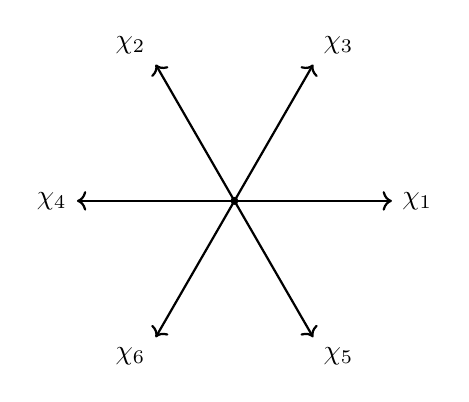
\begin{tikzpicture}
    % Define the root vectors
    \def\l{2} % length of the vectors
    
    % Draw the positive roots
    \draw[->, thick] (0, 0) -- (\l, 0) node[anchor=west] {$\chi_1$};
    \draw[->, thick] (0, 0) -- (-\l/2, \l*0.866) node[anchor=south east] {$\chi_2$};
    \draw[->, thick] (0, 0) -- (-\l/2, -\l*0.866) node[anchor=north east] {$\chi_6$};
    
    % Draw the negative roots
    \draw[->, thick] (0, 0) -- (-\l, 0) node[anchor=east] {$\chi_4$};
    \draw[->, thick] (0, 0) -- (\l/2, -\l*0.866) node[anchor=north west] {$\chi_5$};
    \draw[->, thick] (0, 0) -- (\l/2, \l*0.866) node[anchor=south west] {$\chi_3$};
    
    % Draw the origin
    \fill (0, 0) circle (0.05);
\end{tikzpicture}
\end{center}
\noindent
The condition $\sum_{i=1}^6 a_i \chi_i = 0$ forces $(a_1, \ldots, a_6)$ to lie in the kernel of the matrix
$$
\begin{pmatrix}
	1 & 0 & 1 & -1 & 0 & -1 \\
	-1 & 1 & 0 & 1 & -1 & 0 \\
	0 & -1 & -1 & 0 & 1 & 1
\end{pmatrix}.
$$
The vector space $M_\RR$ is defined as the kernel of this matrix.
The cone corresponding to $V \git T$ is $\sigma = \Span_{\RR_{\ge 0}}\{\bar e_1, \ldots, \bar e_6\}$ in $N_\RR = \RR^6 / M_\RR^\perp.$
We find bases for $M_\RR$ and $M_\RR^\perp$ to understand $\sigma$ concretely.
One verifies $M_\RR$ has dimension 4, and has the following basis:
\begin{align*}
	v_1 &:= \frac{1}{6} (e_1+e_4), & v_2 &:= \frac{1}{6}(e_2+e_5), \\
	v_3 &:= \frac{1}{6}(e_1+e_2+e_6), & v_4 &:= \frac{1}{6}(e_3+e_4+e_5).
\end{align*}
The orthogonal complement $M_\RR^\perp$ is two-dimensional.
It has the following basis:
$$v_5 :=\frac{1}{6}(e_1-e_2-e_4+e_5), \qquad v_6 := \frac{1}{6} (e_1 + e_3 -e_4 - e_6).$$
We have
$$\RR^6 = M_\RR \oplus M_\RR^\perp = \Span_\RR\{v_1, v_2, v_3, v_4\} \oplus \Span_{\RR}\{v_5, v_6\},$$
so we identify $N_\RR = \RR^6 / M_\RR^\perp$ with $\Span_\RR\{v_1, v_2, v_3, v_4\}$.
One can check:
\begin{align*}
	e_1 &= 3v_1 + v_3 - v_4 +v_5+v_6, & e_2 &= 3v_2+v_3-v_4-2v_5+v_6,  \\
	e_3 &= -3v_1-3v_2+2v_3+4v_4-v_5+2v_6,  & e_4 &= 3v_1-v_3+v_4-v_5-v_6, \\
	e_5 &= 3v_2-v_3+v_4+2v_5-v_6, & e_6 &= -3v_1-3v_2+4v_3+2v_4+v_5-2v_6.
\end{align*}
The image of an element in $N_\RR$ is identifed with its projection onto $\Span_\RR\{v_1, v_2, v_3, v_4\}$ under the above decomposition of $\RR^6$.
Thus, the cone $\sigma$ is
\begin{align*}
	\sigma &= \Span_{\RR_{\ge 0}}\{ \bar e_1, \bar e_2, \bar e_3, \bar e_4, \bar e_5, \bar e_6 \} \\
		&= \Span_{\RR_{\ge 0}} \{3v_1 + v_3 - v_4,\,  3v_2+v_3-v_4,\,  -3v_1-3v_2+2v_3+4v_4, \\
		&\qquad\qquad\qquad\qquad  3v_1-v_3+v_4,\,   3v_2-v_3+v_4, \, -3v_1-3v_2+4v_3+2v_4 \}
\end{align*}
in the vector space
$$N_\RR = \Span_\RR\{v_1, v_2, v_3 , v_4\}.$$

\newpage
\hfill








\newpage
\begin{bibdiv}
\begin{biblist}
\bib{AM16}{book}{
   author={Atiyah, M. F.},
   author={Macdonald, I. G.},
   title={Introduction to commutative algebra},
   series={Addison-Wesley Series in Mathematics},
   edition={economy edition},
   note={For the 1969 original see [MR0242802]},
   publisher={Westview Press, Boulder, CO},
   date={2016},
   pages={ix+128},
   isbn={978-0-8133-5018-9},
   isbn={0-201-00361-9},
   isbn={0-201-40751-5},
   review={\MR{3525784}},
}

\bib{BV04}{book}{
   author={Boyd, Stephen},
   author={Vandenberghe, Lieven},
   title={Convex optimization},
   publisher={Cambridge University Press, Cambridge},
   date={2004},
   pages={xiv+716},
   isbn={0-521-83378-7},
   review={\MR{2061575}},
   doi={10.1017/CBO9780511804441},
}

\bib{BM21}{article}{
   author={Bruzzo, Ugo},
   author={Montoya, William},
   title={On the Hodge conjecture for quasi-smooth intersections in toric
   varieties},
   journal={S\~ao Paulo J. Math. Sci.},
   volume={15},
   date={2021},
   number={2},
   pages={682--694},
   issn={1982-6907},
   review={\MR{4341124}},
   doi={10.1007/s40863-021-00247-y},
}


\bib{Cassels97}{book}{
   author={Cassels, J. W. S.},
   title={An introduction to the geometry of numbers},
   series={Classics in Mathematics},
   note={Corrected reprint of the 1971 edition},
   publisher={Springer-Verlag, Berlin},
   date={1997},
   pages={viii+344},
   isbn={3-540-61788-4},
   review={\MR{1434478}},
}

\bib{CLS11}{book}{
   author={Cox, David A.},
   author={Little, John B.},
   author={Schenck, Henry K.},
   title={Toric varieties},
   series={Graduate Studies in Mathematics},
   volume={124},
   publisher={American Mathematical Society, Providence, RI},
   date={2011},
   pages={xxiv+841},
   isbn={978-0-8218-4819-7},
   review={\MR{2810322}},
   doi={10.1090/gsm/124},
}

\bib{DLHK13}{book}{
   author={De Loera, Jes\'us A.},
   author={Hemmecke, Raymond},
   author={K\"oppe, Matthias},
   title={Algebraic and geometric ideas in the theory of discrete
   optimization},
   series={MOS-SIAM Series on Optimization},
   volume={14},
   publisher={Society for Industrial and Applied Mathematics (SIAM),
   Philadelphia, PA; Mathematical Optimization Society, Philadelphia, PA},
   date={2013},
   pages={xx+322},
   isbn={978-1-611972-43-6},
   review={\MR{3024570}},
}

\bib{DC70}{article}{
   author={Dieudonn\'e, Jean A.},
   author={Carrell, James B.},
   title={Invariant theory, old and new},
   journal={Advances in Math.},
   volume={4},
   date={1970},
   pages={1--80 (1970)},
   issn={0001-8708},
   review={\MR{0255525}},
   doi={10.1016/0001-8708(70)90015-0},
}

\bib{Dolgachev03}{book}{
   author={Dolgachev, Igor},
   title={Lectures on invariant theory},
   series={London Mathematical Society Lecture Note Series},
   volume={296},
   publisher={Cambridge University Press, Cambridge},
   date={2003},
   pages={xvi+220},
   isbn={0-521-52548-9},
   review={\MR{2004511}},
   doi={10.1017/CBO9780511615436},
}

\bib{FSR17}{book}{
   author={Ferrer Santos, Walter Ricardo},
   author={Rittatore, Alvaro},
   title={Actions and invariants of algebraic groups},
   series={Monographs and Research Notes in Mathematics},
   edition={2},
   publisher={CRC Press, Boca Raton, FL},
   date={2017},
   pages={xx+459},
   isbn={978-1-4822-3915-7},
   review={\MR{3617213}},
   doi={10.1201/9781315118482},
}

\bib{Fulton93}{book}{
   author={Fulton, William},
   title={Introduction to toric varieties},
   series={Annals of Mathematics Studies},
   volume={131},
   note={The William H. Roever Lectures in Geometry},
   publisher={Princeton University Press, Princeton, NJ},
   date={1993},
   pages={xii+157},
   isbn={0-691-00049-2},
   review={\MR{1234037}},
   doi={10.1515/9781400882526},
}

\bib{Geck13}{book}{
   author={Geck, Meinolf},
   title={An introduction to algebraic geometry and algebraic groups},
   series={Oxford Graduate Texts in Mathematics},
   volume={20},
   note={First paperback reprinting of the 2003 original},
   publisher={Oxford University Press, Oxford},
   date={2013},
   pages={xii+307},
   isbn={978-0-19-967616-3},
   review={\MR{3086289}},
}

\bib{Hartshorne77}{book}{
   author={Hartshorne, Robin},
   title={Algebraic geometry},
   series={Graduate Texts in Mathematics},
   volume={No. 52},
   publisher={Springer-Verlag, New York-Heidelberg},
   date={1977},
   pages={xvi+496},
   isbn={0-387-90244-9},
   review={\MR{0463157}},
}

\bib{Hilbert90}{article}{
   author={Hilbert, David},
   title={Ueber die Theorie der algebraischen Formen},
   language={German},
   journal={Math. Ann.},
   volume={36},
   date={1890},
   number={4},
   pages={473--534},
   issn={0025-5831},
   review={\MR{1510634}},
   doi={10.1007/BF01208503},
}

\bib{Humphreys75}{book}{
   author={Humphreys, James E.},
   title={Linear algebraic groups},
   series={Graduate Texts in Mathematics},
   volume={No. 21},
   publisher={Springer-Verlag, New York-Heidelberg},
   date={1975},
   pages={xiv+247},
   review={\MR{0396773}},
}

\bib{Kamgarpour21}{webpage}{
   author={Kamgarpour, Masoud},
   title={UQ Maths Stradbroke Island Workshop on Character Varieties},
   date={2021},
   note={Available at \url{https://baileywhitbread.com/files/21_character_varieties.pdf}}
}

\bib{Milne23}{webpage}{
   author={Milne, James S.},
   title={Algebraic Geometry (v6.03)},
   date={2023},
   note={Available at \url{www.jmilne.org/math/}}
}

\bib{Mukai03}{book}{
   author={Mukai, Shigeru},
   title={An introduction to invariants and moduli},
   series={Cambridge Studies in Advanced Mathematics},
   volume={81},
   edition={Japanese edition},
   publisher={Cambridge University Press, Cambridge},
   date={2003},
   pages={xx+503},
   isbn={0-521-80906-1},
   review={\MR{2004218}},
}

\bib{Mumford65}{book}{
   author={Mumford, David},
   title={Geometric invariant theory},
   series={Ergebnisse der Mathematik und ihrer Grenzgebiete, (N.F.)},
   volume={Band 34},
   publisher={Springer-Verlag, Berlin-New York},
   date={1965},
   pages={vi+145},
   review={\MR{0214602}},
}

\bib{Nagata60}{article}{
   author={Nagata, Masayoshi},
   title={On the fourteenth problem of Hilbert},
   conference={
      title={Proc. Internat. Congress Math. 1958},
   },
   book={
      publisher={Cambridge Univ. Press, New York},
   },
   date={1960},
   pages={459--462},
   review={\MR{0116056}},
}

\bib{Oda88}{book}{
   author={Oda, Tadao},
   title={Convex bodies and algebraic geometry},
   series={Ergebnisse der Mathematik und ihrer Grenzgebiete (3) [Results in
   Mathematics and Related Areas (3)]},
   volume={15},
   note={An introduction to the theory of toric varieties;
   Translated from the Japanese},
   publisher={Springer-Verlag, Berlin},
   date={1988},
   pages={viii+212},
   isbn={3-540-17600-4},
   review={\MR{0922894}},
}

\bib{Proudfoot05}{article}{
author={Proudfoot, Nicholas J.},
title={Geometric invariant theory and projective toric varieties},
year={2005},
note={Preprint, \href{https://arxiv.org/abs/math/0502366}{arXiv:math/0502366}}
}

\bib{Reid88}{book}{
   author={Reid, Miles},
   title={Undergraduate algebraic geometry},
   series={London Mathematical Society Student Texts},
   volume={12},
   publisher={Cambridge University Press, Cambridge},
   date={1988},
   pages={viii+129},
   isbn={0-521-35559-1},
   isbn={0-521-35662-8},
   review={\MR{0982494}},
   doi={10.1017/CBO9781139163699},
}

\bib{Reid95}{book}{
   author={Reid, Miles},
   title={Undergraduate commutative algebra},
   series={London Mathematical Society Student Texts},
   volume={29},
   publisher={Cambridge University Press, Cambridge},
   date={1995},
   pages={xiv+153},
   isbn={0-521-45255-4},
   review={\MR{1458066}},
   doi={10.1017/CBO9781139172721},
}

\bib{Serre73}{book}{
   author={Serre, J.-P.},
   title={A course in arithmetic},
   series={Graduate Texts in Mathematics},
   volume={No. 7},
   note={Translated from the French},
   publisher={Springer-Verlag, New York-Heidelberg},
   date={1973},
   pages={viii+115},
   review={\MR{0344216}},
}

\bib{Springer98}{book}{
   author={Springer, T. A.},
   title={Linear algebraic groups},
   series={Progress in Mathematics},
   volume={9},
   edition={2},
   publisher={Birkh\"auser Boston, Inc., Boston, MA},
   date={1998},
   pages={xiv+334},
   isbn={0-8176-4021-5},
   review={\MR{1642713}},
   doi={10.1007/978-0-8176-4840-4},
}

\bib{Stillwell20}{book}{
   author={Stillwell, John},
   title={Mathematics and its history},
   series={Undergraduate Texts in Mathematics},
   edition={concise edition},
   publisher={Springer, Cham},
   date={2020},
   pages={xv+399},
   isbn={978-3-030-55193-3},
   isbn={978-3-030-55192-6},
   review={\MR{4174697}},
   doi={10.1007/978-3-030-55193-3},
}

\bib{Zaman13}{webpage}{
   author={Zaman, Ragib},
   title={Geometry and Topology of Toric Varieties},
   date={2013},
   note={Available at \url{https://github.com/RagibZaman/Toric-Varieties}}
}
\end{biblist}
\end{bibdiv}
\end{document}
